% ========================================= TEMPLATE INFO ========================================
%
% Author:       P4ntomime
% Version:      1.0.0
% Last updated: 2024-02-18
% Brief:        A LaTeX template for summaries. See README.md for more information.
% 
% ================================================================================================
\documentclass[8pt, a4paper, twoside, landscape]{extarticle}
% Font size:    8pt
% Paper size:   A4
% style:        twoside (needed, so odd and even pages have different margins)
% orientation:  portrait. (use 'landscape' for landscape orientation)


% ========================================= DOCUMENT INFO =========================================
\def\title{Leistungselektronik}       % title
\def\shorttitle{Leistungselektronik}                            % short title (displayed as PDF title)
\def\dozent{Dr. Jasmin Smajic }               % docent
\def\semester{HS 2025}                              % semester
\def\author{Gian Marco Näf}                           % author(s)
\def\repo{https://github.com/Giamo08/Zusammenfassungen}        % repository link
\def\version{1.0.\today}                            % version
\def\pagelimit{30}                                   % page limit -> causes pages after limit to be red
\def\titleoption{ultra compact}                     % options: ultra compact, compact, normal
\def\enableToC{false}

% ================================= PACKAGES, SETUP AND COMMANDS ==================================
\input{preamble.tex}
\makeatletter
\def\@enableToC{true}
\ifx\enableToC\@enableToC
    \setcounter{tocdepth}{2} % adjust depth: 0=parts,1=sections,2=subsections,...
    \AtBeginDocument{%
        \clearpage
        \tableofcontents
        \clearpage
    }
\fi
\makeatother

% =========================================== DOCUMENT ============================================
\begin{document}

    \begin{layout}
        \section{Grundlagen zeitkontinuierlicher Systeme}

Ein \textbf{zeitkontinuierliches System} beschreibt den Zusammenhang zwischen einer Eingangsgrösse $u(t)$ und einer Ausgangsgrösse $y(t)$
für eine kontinuierliche Zeitvariable $t \in \mathbb{R}$.
In der Leistungselektronik ist das typischerweise der Lastkreis (z.B.\ $R$-$L$, $R$-$C$, $R$-$L$-$C$), der durch \textbf{Differentialgleichungen}
modelliert wird.

\smallskip

\textbf{Zielbild (Outcome):}
\begin{itemize}
    \item Modell aufsetzen (DGL oder Zustandsraum)
    \item Zeitverlauf berechnen (Einschwingen, Ausschwingen, Umschalten)
    \item Kennwerte ableiten (Mittelwert, Effektivwert, Leistung, Ripple, Zeitkonstante)
    \item Stationären Betrieb bestimmen (periodisch, eingeschwungen)
\end{itemize}

\subsection{Systembegriffe und Klassifikation}

\subsubsection{Eingang, Ausgang, Zustand}
\begin{itemize}
    \item \textbf{Eingang} $u(t)$: Anregung von aussen (z.B.\ Quelle, PWM, Schalterstellung).
    \item \textbf{Ausgang} $y(t)$: beobachtete Grösse (z.B.\ Laststrom $i(t)$, Lastspannung $u_R(t)$).
    \item \textbf{Zustand} $x(t)$: minimaler Satz interner Variablen, der zusammen mit $u(t)$ die Zukunft vollständig bestimmt.
          In elektrischen Netzwerken sind Zustände typischerweise \textbf{Induktorströme} und \textbf{Kondensatorspannungen}.
\end{itemize}

\subsubsection{Linearität}
Ein System ist \textbf{linear}, wenn \textbf{Superposition} gilt:
\[
u_1(t)\rightarrow y_1(t),\; u_2(t)\rightarrow y_2(t)\quad \Rightarrow \quad
\alpha u_1(t)+\beta u_2(t)\rightarrow \alpha y_1(t)+\beta y_2(t).
\]
Lineare Modelle sind der Standard für $R$-$L$-$C$-Netze (bei idealen Bauteilen und ohne Sättigung).

\subsubsection{Zeitinvarianz}
Ein System ist \textbf{zeitinvariant}, wenn eine Zeitverschiebung am Eingang dieselbe Zeitverschiebung am Ausgang erzeugt:
\[
u(t-t_0)\rightarrow y(t-t_0).
\]
Ein \textbf{LTI-System} (linear time-invariant) ist der Kernfall für analytische Lösungen (Faltung, Laplace, Frequenzgang).

\subsubsection{Kausalität}
\textbf{Kausal} bedeutet: $y(t)$ hängt nur von $u(\tau)$ für $\tau \le t$ ab.
Physikalische elektrische Systeme sind kausal.

\subsubsection{Stabilität (praktisch relevant)}
\begin{itemize}
    \item \textbf{BIBO-stabil}: beschränkter Eingang $\Rightarrow$ beschränkter Ausgang.
    \item Für LTI-Systeme entspricht das (bei rationalen Übertragungsfunktionen) Polen mit negativer Realteil-Lage.
\end{itemize}

\subsection{Mathematische Modellierung}

\subsubsection{Differentialgleichungen als Systemmodell}
Viele zeitkontinuierliche Systeme werden durch eine lineare DGL beschrieben:
\[
a_n \frac{d^n y}{dt^n} + \dots + a_1 \frac{dy}{dt} + a_0 y
=
b_m \frac{d^m u}{dt^m} + \dots + b_1 \frac{du}{dt} + b_0 u.
\]
In der Leistungselektronik dominieren häufig Systeme \textbf{1.\ Ordnung} (z.B.\ $R$-$L$ oder $R$-$C$) und \textbf{2.\ Ordnung} (z.B.\ $L$-$C$ mit Dämpfung).

\subsubsection{Zustandsraumdarstellung}
Alternative Standardform (skalierbar, schaltertauglich):
\[
\dot{x}(t)=A x(t)+B u(t), \qquad y(t)=C x(t)+D u(t).
\]
\textbf{Use-Case:} Bei Schaltvorgängen ändert sich typischerweise $A,B,C,D$ stückweise (Topologie 1, Topologie 2, \dots).
Das ist der saubere Rahmen für \textbf{stückweise lineare} Systeme.

\subsection{Systeme 1.\ Ordnung (Business Case: $R$-$L$ und $R$-$C$)}

\subsubsection{$R$-$L$-System}
Grundgleichung (typisch in Übungen):
\[
u(t)=R\,i(t)+L\,\frac{di(t)}{dt}.
\]
Zeitkonstante:
\[
\cbl{\tau=\frac{L}{R}}
\]
Interpretation: Nach ca.\ $t=5\tau$ ist ein Einschwingvorgang praktisch abgeschlossen (ca.\ 99\%).

\subsubsection{$R$-$C$-System}
Grundgleichung:
\[
i(t)=C\frac{du_C(t)}{dt},\qquad u(t)=u_R(t)+u_C(t)=R i(t)+u_C(t).
\]
Zeitkonstante:
\[
\cbl{\tau=R C}
\]

\subsection{Lösungskonzept für lineare DGL 1.\ Ordnung}

Standardform:
\[
\frac{dy}{dt}+a\,y=b\,u(t).
\]

\subsubsection{Homogene Lösung (natürliche Antwort)}
Setze $u(t)=0$:
\[
\frac{dy_h}{dt}+a\,y_h=0 \quad \Rightarrow \quad y_h(t)=K\,e^{-a t}.
\]
\textbf{Interpretation:} Das System trägt Energie ab. Exponentielles Abklingen.

\subsubsection{Partikuläre Lösung (erzwungene Antwort)}
Für einen konstanten Eingang $u(t)=U_0$:
\[
\frac{dy_p}{dt}+a\,y_p=b\,U_0.
\]
Typischer Ansatz: $y_p=\text{konstant}$.
Dann ergibt sich der Endwert:
\[
y_\infty=\frac{b}{a}U_0.
\]

\subsubsection{Gesamtlösung}
\[
y(t)=y_p(t)+y_h(t).
\]
Für den konstanten Eingang ist das die klassische Einschwingform:
\[
\cbl{y(t)=y_\infty + \big(y(0)-y_\infty\big)\,e^{-t/\tau}}
\]
Hier gilt $\tau=1/a$.

\subsubsection{Initialbedingungen und Kontinuität}
\begin{itemize}
    \item \textbf{Induktorstrom ist stetig:} $\cbl{i_L(t^-)=i_L(t^+)}$ (Strom kann nicht sprunghaft ändern, sonst bräuchte man unendliche Spannung).
    \item \textbf{Kondensatorspannung ist stetig:} $\cbl{u_C(t^-)=u_C(t^+)}$ (Spannung kann nicht sprunghaft ändern, sonst bräuchte man unendlichen Strom).
\end{itemize}
Diese Kontinuitätsregeln sind bei \textbf{Schaltvorgängen} die zentrale Randbedingung zur Bestimmung der Integrationskonstanten.

\subsection{Stückweise Systeme bei Schaltbetrieb (Topologie-Wechsel)}

In Schaltungen mit Schaltern gilt oft:
\[
\text{Topologie 1: } \dot{x}=A_1 x + B_1 u,\quad t\in[t_0,t_1)
\]
\[
\text{Topologie 2: } \dot{x}=A_2 x + B_2 u,\quad t\in[t_1,t_2)
\]
\textbf{Vorgehen:}
\begin{enumerate}
    \item Pro Zeitintervall DGL lösen (typisch exponentiell).
    \item Übergangsbedingungen am Schaltzeitpunkt mit Kontinuität ansetzen.
    \item Bei periodischem Betrieb zusätzlich Periodizität verlangen:
    \[
    x(t_0)=x(t_0+T_s)
    \]
    \item Daraus Integrationskonstanten bestimmen.
\end{enumerate}

\subsection{Stationärer Betrieb vs.\ Transient}

\subsubsection{Transient (Einschwingen)}
Startbedingungen sind relevant. Lösung enthält $e^{-t/\tau}$-Anteile, die mit der Zeit verschwinden.

\subsubsection{Stationär (eingeschwungen)}

\crd{\textrightarrow\ Stationär bedeutet periodisch wiederholbar, nicht konstant.}

Die natürlichen Anteile sind ``abgebaut''. Im periodischen Schaltbetrieb bedeutet stationär:
\[
\cbl{x(t)=x(t+T_s)}
\]
Wichtig: Stationär heisst nicht konstant, sondern \textbf{periodisch wiederholbar}.

\subsection{Übertragungsfunktion und Laplace }

\subsubsection{Laplace-Transformation}
Für LTI-Systeme ist Laplace ein Standard-Werkzeug zur Formalisierung von Dynamik:
\[
\cbl{\mathcal{L}\{f(t)\}=F(s)=\int_0^\infty f(t)\,e^{-st}\,dt}
\]

\subsubsection{Übertragungsfunktion}
Bei Nullanfangsbedingungen:
\[
\cbl{G(s)=\frac{Y(s)}{U(s)}}
\]
Für $R$-$L$ mit Ausgang $i(t)$ und Eingang $u(t)$:
\[
\cbl{G(s)=\frac{I(s)}{U(s)}=\frac{1}{R+Ls}}
\]
Pol:
\[
\cbl{s=-\frac{R}{L}}
\]
\textbf{Interpretation:} Negative Pol-Lage $\Rightarrow$ stabil, exponentielles Abklingen.

\subsubsection{Impulsantwort und Faltung}
Für LTI gilt:
\[
y(t)=(g*u)(t)=\int_{0}^{t} g(\tau)\,u(t-\tau)\,d\tau,
\]
wobei $g(t)$ die Impulsantwort ist.
In der Leistungselektronik wird das oft indirekt genutzt (Filterwirkung, Glättung, Spektralargumentation).

\subsection{Kennwerte im Zeitbereich (Operational KPIs)}

\subsubsection{Mittelwert (DC-Anteil)}
Für periodische Signale:
\[
\cbl{\overline{x}=\frac{1}{T}\int_{0}^{T} x(t)\,dt}
\]

\subsubsection{Effektivwert (RMS)}
\[
\cbl{X_{\mathrm{RMS}}=\sqrt{\frac{1}{T}\int_{0}^{T} x^2(t)\,dt}}
\]
\textbf{Use-Case:} Thermische Bewertung und Leistungsberechnung.

\subsubsection{Wirkleistung}
\[
\cbl{p(t)=u(t)\,i(t),\qquad P=\overline{p(t)}=\frac{1}{T}\int_0^T u(t)i(t)\,dt}
\]
Für ohmsche Last:
\[
P=R\,I_{\mathrm{RMS}}^2=\frac{U_{\mathrm{RMS}}^2}{R}.
\]

\subsection{Typische Fehlerbilder (Quality Gate)}

\crd{Diese Punkte sind typische Prüfungsfallen.}

\begin{itemize}
    \item Kontinuität falsch angesetzt (Induktorstrom oder Kondensatorspannung springt).
    \item Stationär mit konstant verwechselt (periodisch vs.\ DC).
    \item Zeitvariable im Exponenten falsch skaliert (fehlende $\tau$, falsches Vorzeichen).
    \item Periodenbedingungen nicht geschlossen (Integrationskonstanten bleiben frei).
    \item RMS und Mittelwert vermischt (insbesondere bei nichtsinusförmigen Signalen).
\end{itemize}

\subsection{Minimal-Checkliste für Aufgaben (Execution Plan)}
\begin{enumerate}
    \item Topologie pro Zeitintervall identifizieren.
    \item DGL aufstellen (KVL/KCL).
    \item Standardform erkennen ($1.\ Ordnung$: exponentiell).
    \item Anfangs- und Übergangsbedingungen definieren (Kontinuität).
    \item Bei stationär-periodisch: $x(t)=x(t+T_s)$ einsetzen.
    \item Gesuchte Grössen ableiten: $u_R=Ri$, $u_L=L\,di/dt$, Leistung, RMS, Mittelwert.
\end{enumerate}

        \section{Leistungshalbleiter in der Leistungselektronik}

\subsection{Rolle der Leistungshalbleiter im Energiesystem}

Leistungshalbleiter dienen der verlustarmen, schnellen und steuerbaren Umsetzung elektrischer Energie.
Sie arbeiten im Gegensatz zu linearen Bauelementen ausschliesslich in den Zuständen:
\begin{itemize}
\item \textbf{leitend} (niedriger Spannungsabfall),
\item \textbf{sperrend} (hohe Sperrspannung),
\item \textbf{umschaltend} (Übergangszustand).
\end{itemize}

Damit realisieren sie:
\begin{itemize}
\item Gleichrichtung,
\item Phasenanschnitt,
\item Taktbetrieb (PWM),
\item Umrichtung von Spannung, Strom und Frequenz.
\end{itemize}

Grundlegende Kenngrössen:
\[
U_{RRM},\quad I_{F},\quad U_F,\quad t_{on},\ t_{off},\quad P_{cond},\ P_{sw}.
\]

\subsection{Physikalische Grundlagen der Halbleiterbauelemente}

Alle Leistungshalbleiter beruhen auf pn-Übergängen.

Sperrbetrieb:
\[
i \approx 0,\qquad u \le U_{RRM}
\]

Durchlassbetrieb:
\[
i \gg 0,\qquad u \approx U_{on}
\]

Die maximale Sperrspannung wird bestimmt durch:
\begin{itemize}
\item Dicke der Sperrschicht,
\item Dotierung,
\item Feldverteilung im pn-Übergang.
\end{itemize}

Thermische Belastung:
\[
\boxed{T_j = T_{amb} + R_{th} \cdot P_V}
\]
mit:
\begin{itemize}
\item $T_j$: Sperrschichttemperatur,
\item $R_{th}$: thermischer Widerstand,
\item $P_V$: Verlustleistung.
\end{itemize}

\subsection{Diode als Leistungsschalter}

\subsubsection{Betriebszustände}

Die Leistungsdiode besitzt zwei stabile Zustände:

\textbf{Durchlass:}
\[
u_D > 0,\qquad i_D > 0
\]

\textbf{Sperre:}
\[
u_D < 0,\qquad i_D \approx 0
\]

Ideales Modell:
\[
u_D =
\begin{cases}
0, & i_D > 0 \\
\infty, & i_D = 0
\end{cases}
\]

\subsubsection{Statisches Durchlassmodell}

Reales Modell:
\[
\boxed{u_D = U_{D0} + r_D \, i_D}
\]

Verlustleistung:
\[
\boxed{P_D = U_{D0} \, I_{D,\mathrm{avg}} + r_D \, I_{D,\mathrm{RMS}}^2}
\]

Interpretation:
\begin{itemize}
\item $U_{D0}$ dominiert bei kleinen Strömen,
\item $r_D$ dominiert bei grossen Strömen.
\end{itemize}

\begin{center}
    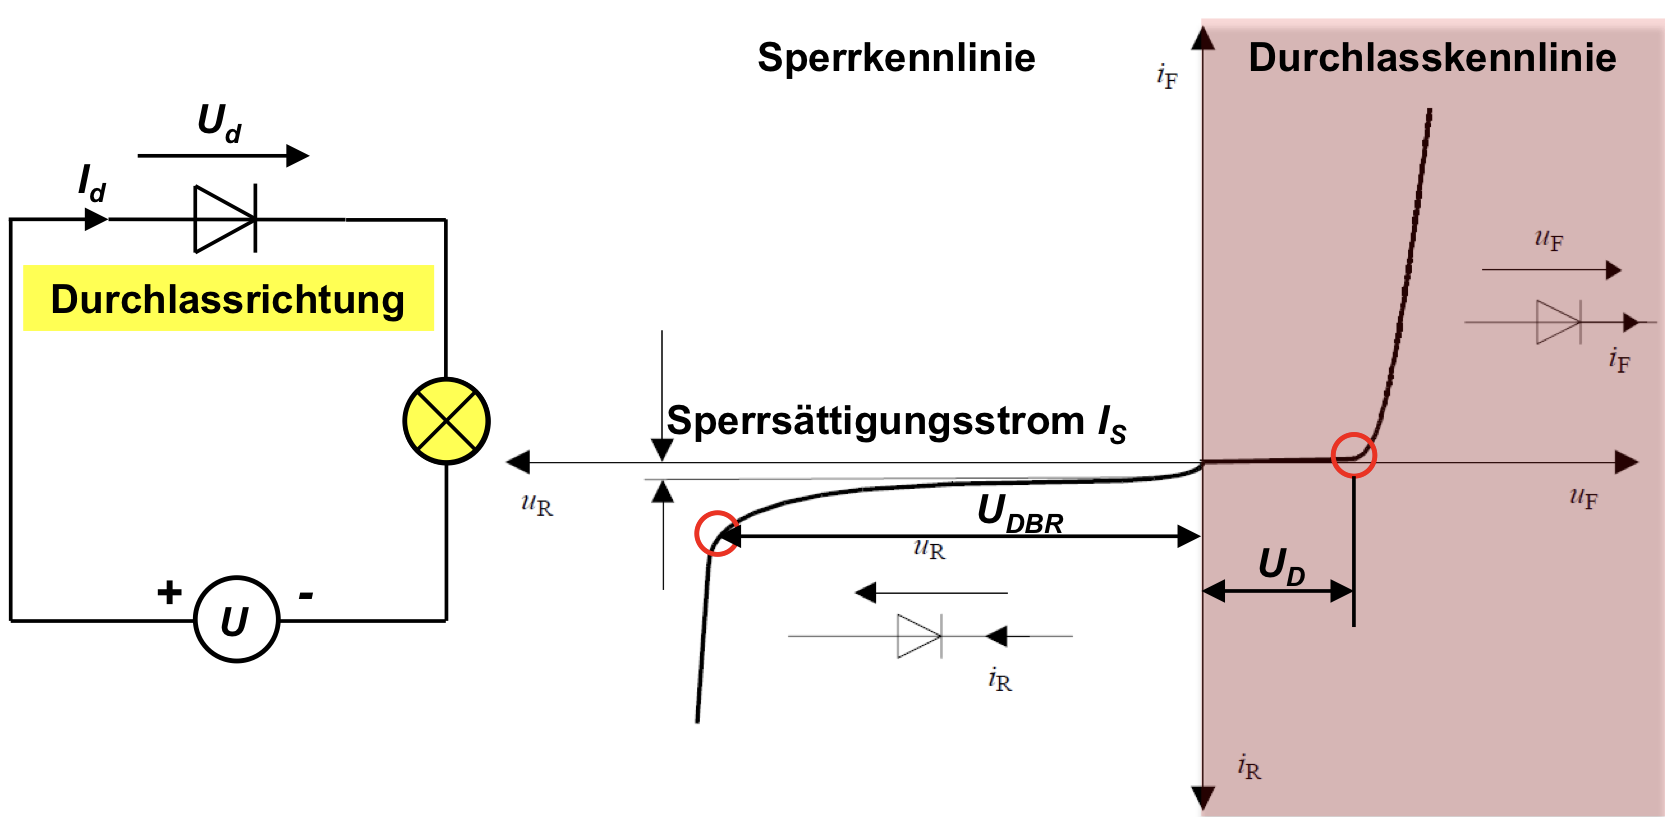
\includegraphics[width=0.85\linewidth]{images/Didodekennlinie.png}
\end{center}
\begin{center}
    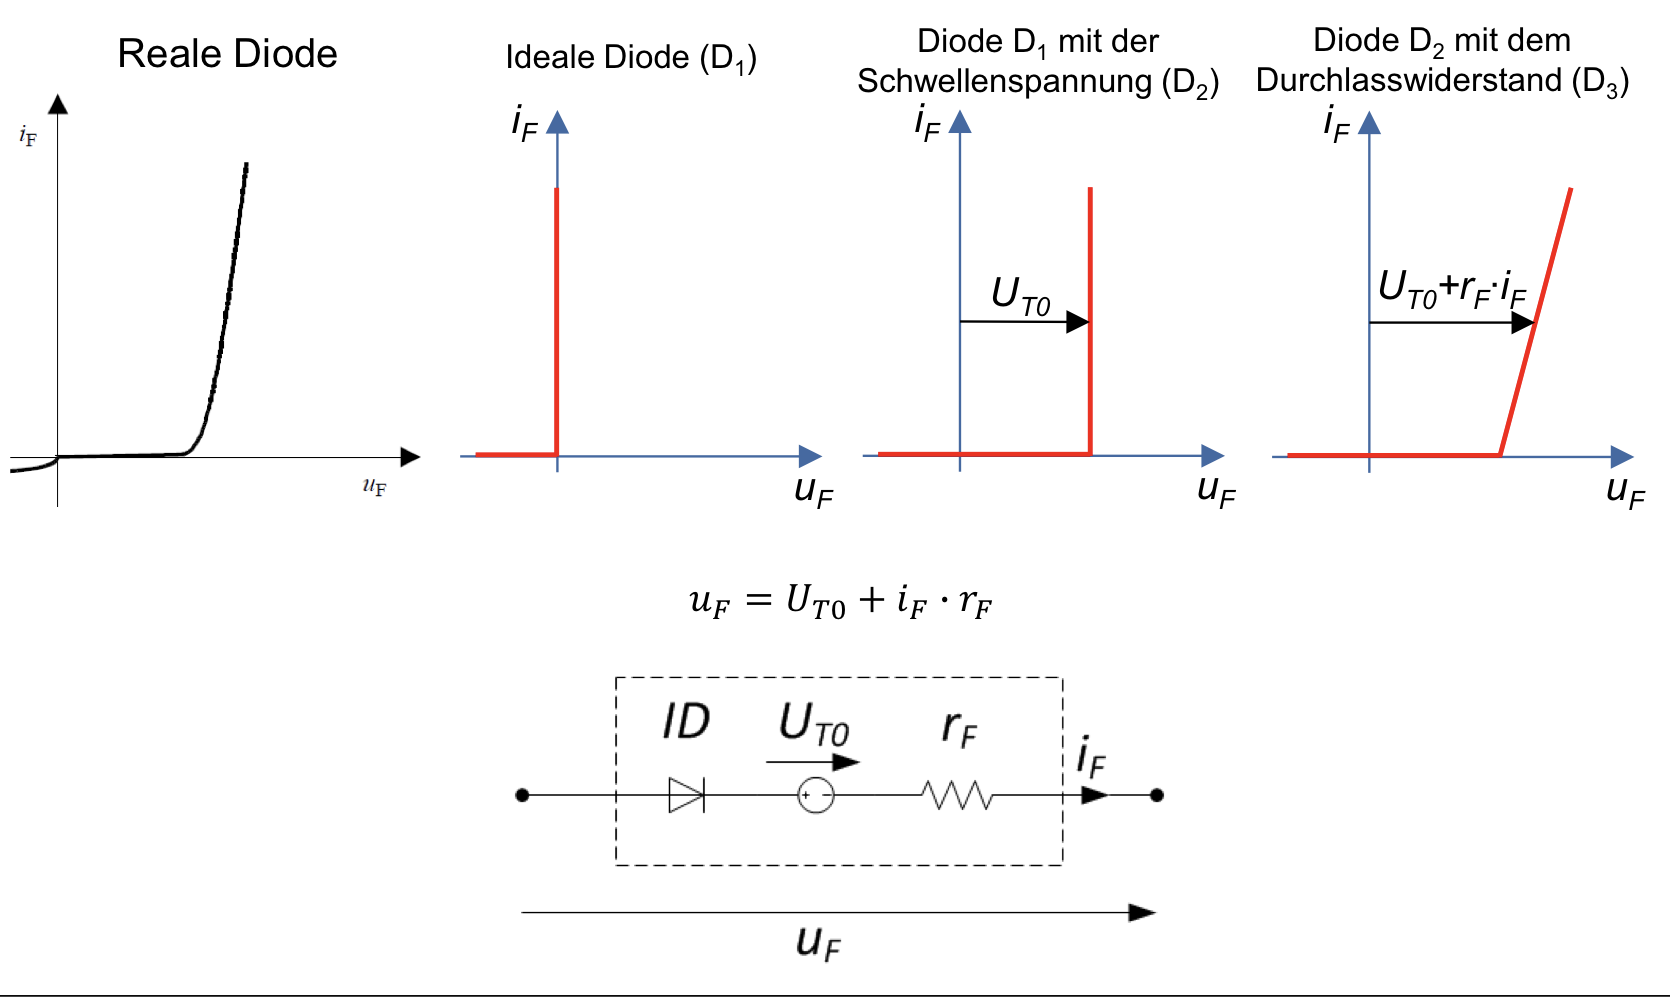
\includegraphics[width=0.85\linewidth]{images/didodeunterschied.png}
\end{center}
\subsubsection{Dynamisches Schaltverhalten}

Beim Übergang von Durchlass nach Sperre wird Ladung aus der Sperrschicht entfernt.

Rückerholstrom:
\[
i_{rr}(t)
\]

Rückerholladung:
\[
\boxed{Q_{rr} = \int_0^{t_{rr}} i_{rr}(t)\,dt}
\]

Zusätzliche Schaltverluste:
\[
\boxed{P_{sw,D} \approx f_s \, U_R \, Q_{rr}}
\]

Physikalische Bedeutung:
\begin{itemize}
\item grosse $Q_{rr}$ $\Rightarrow$ hohe Verluste,
\item schnelle Dioden notwendig für hohe $f_s$.
\end{itemize}

\begin{center}
    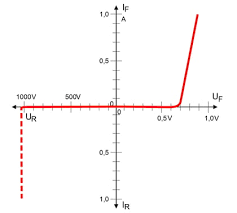
\includegraphics[width=0.85\linewidth]{images/rueckerhol.png}
\end{center}

\subsection{Thyristor (SCR)}

\subsubsection{Vier-Schichten-Struktur und Zündprinzip}

Der Thyristor besitzt eine PNPN-Struktur.

Zündbedingung:
\[
u_{AK} > 0 \quad \text{und} \quad i_G > 0
\]

Nach dem Zünden:
\[
\boxed{\text{Selbsthaltung durch innere Rückkopplung}}
\]

Haltestrom:
\[
\boxed{i_A > I_H}
\]

Abschalten nur durch:
\begin{itemize}
\item Stromnulldurchgang,
\item externe Kommutierung.
\end{itemize}

\begin{center}
    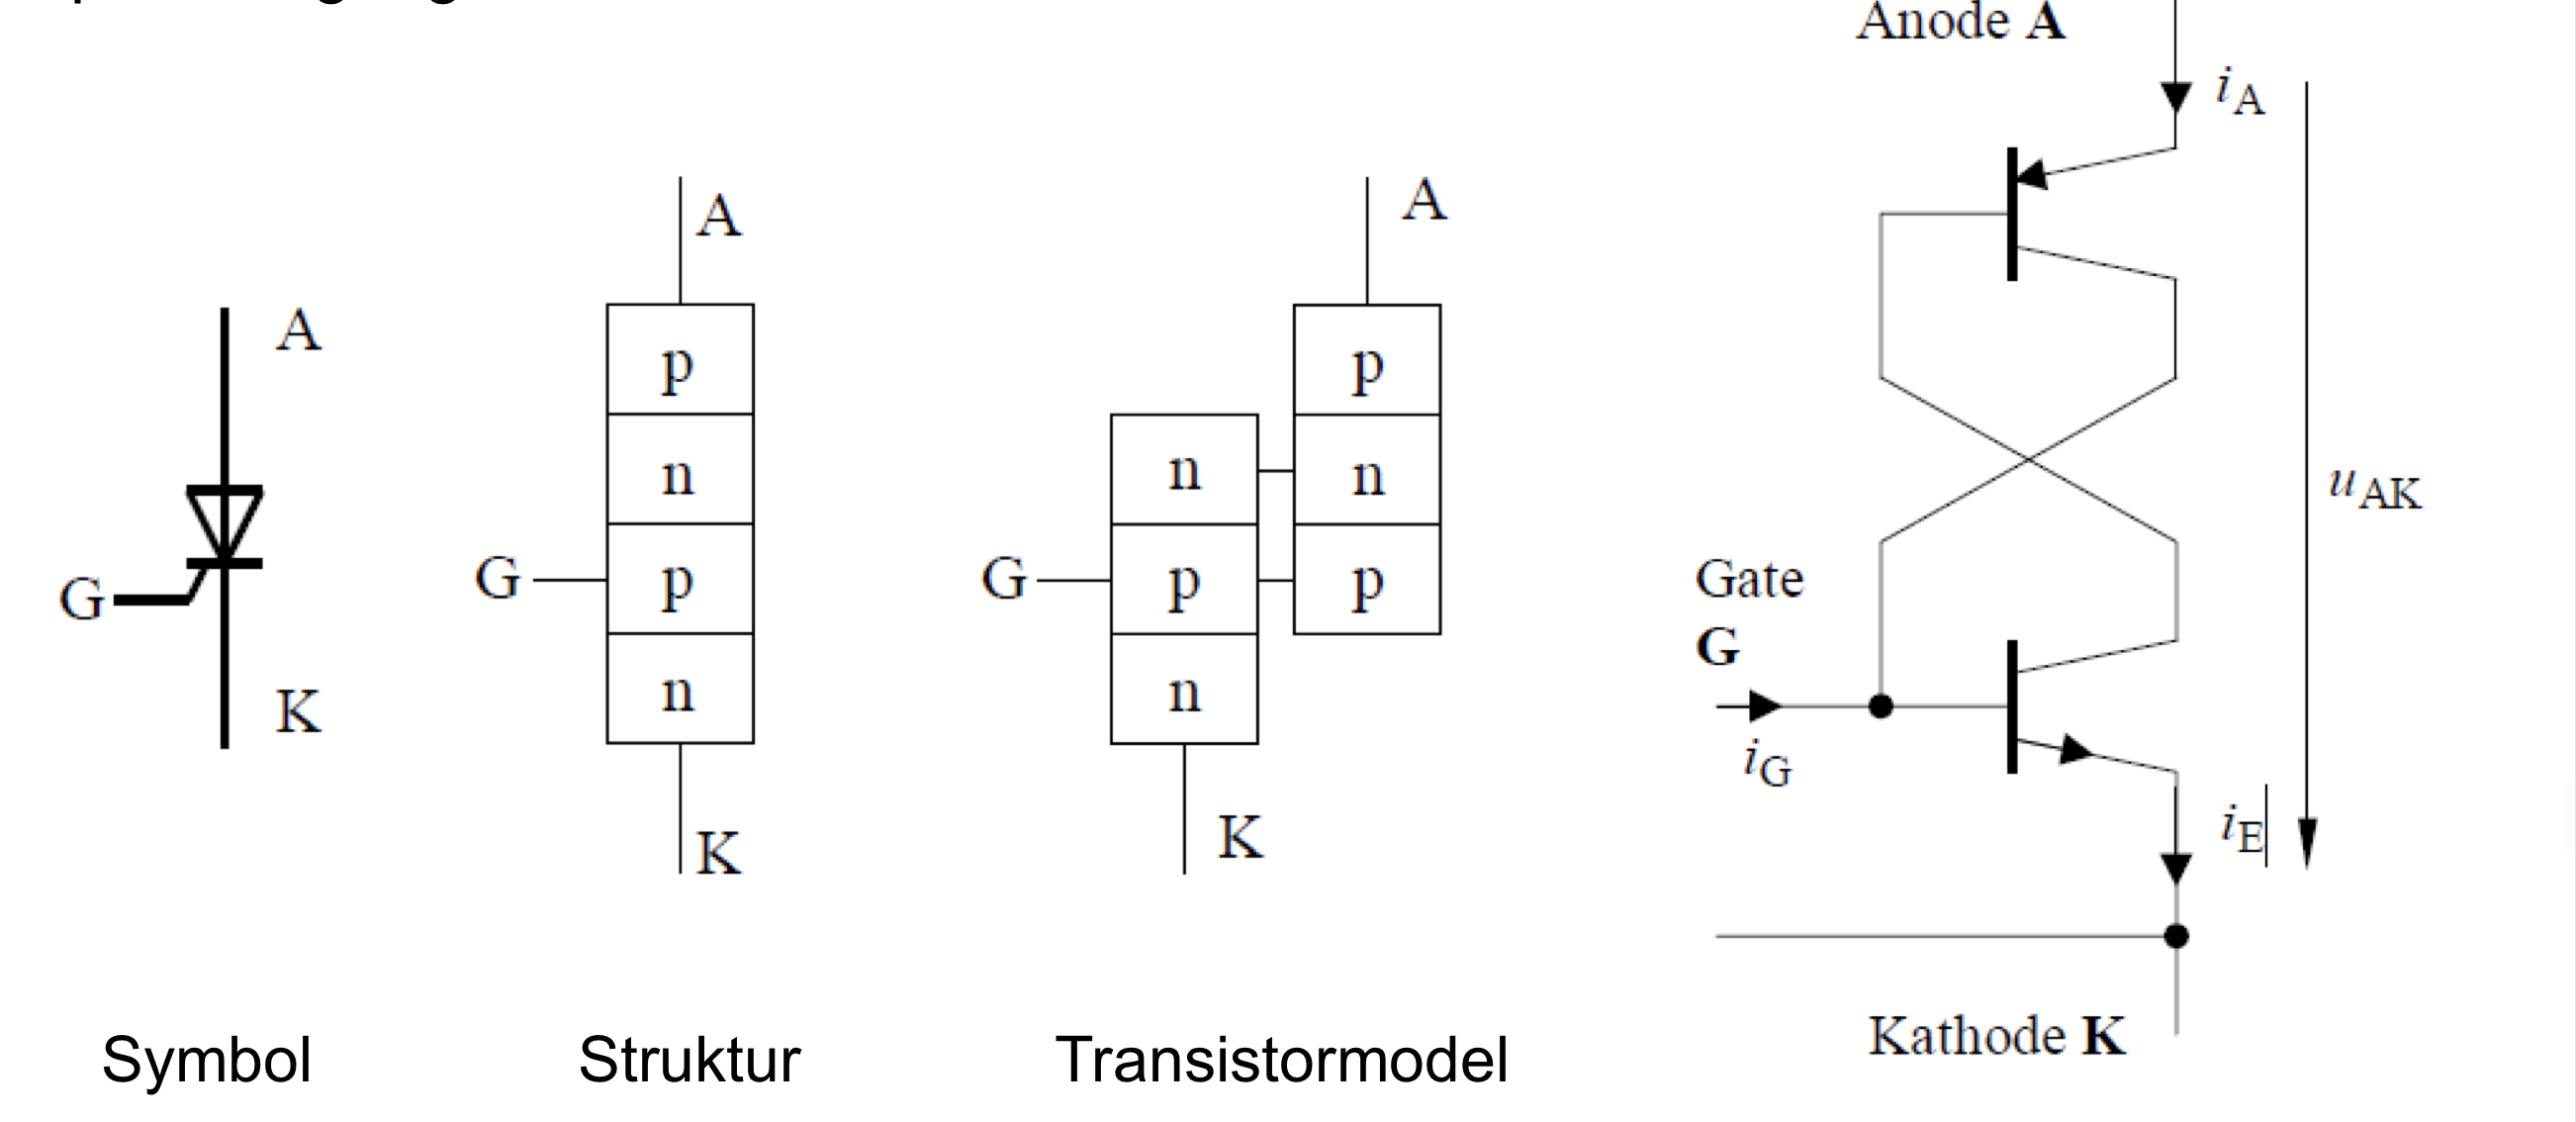
\includegraphics[width=0.85\linewidth]{images/thyristor.png}
\end{center}

\subsubsection{Statisches Modell und Verluste}

\[
\boxed{u_T = U_{T0} + r_T \, i_T}
\]

\[
\boxed{P_T = U_{T0} \, I_{T,\mathrm{avg}} + r_T \, I_{T,\mathrm{RMS}}^2}
\]

Zusätzliche Kenngrössen:
\[
\frac{di}{dt}_{\max},\qquad \frac{du}{dt}_{\max}
\]

Bedeutung:
\begin{itemize}
\item Begrenzen Zündstromanstieg,
\item Schutz durch Snubber notwendig.
\end{itemize}

\subsection{Leistungs-MOSFET}

\subsubsection{Gate-gesteuerter Feldeffekttransistor}

Leitbedingung:
\[
\boxed{u_{GS} > U_{th}}
\]

Im leitenden Zustand:
\[
\boxed{u_{DS} = r_{DS,on} \, i_D}
\]

Charakteristisch:
\begin{itemize}
\item Mehrheitsladungsträger,
\item kein Speicherladungseffekt,
\item sehr schnelles Schalten.
\end{itemize}

\begin{center}
    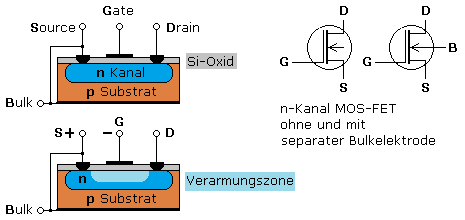
\includegraphics[width=0.85\linewidth]{images/MOSFET.png}
\end{center}

\subsubsection{Dynamisches Modell und Gate-Ladung}

Gate-Ladung:
\[
Q_G = Q_{GS} + Q_{GD}
\]

Schaltzeit:
\[
t_{on} \approx \frac{Q_G}{I_G}
\]

Schaltverluste:
\[
\boxed{P_{sw,M} \approx f_s \int u_{DS}(t)i_D(t)\,dt}
\]

\subsection{IGBT}

\subsubsection{Hybridstruktur MOS–Bipolar}

Der IGBT kombiniert:
\begin{itemize}
\item spannungsgesteuertes MOS-Gate,
\item stromtragende bipolare Struktur.
\end{itemize}

Leitbedingung:
\[
\boxed{u_{GE} > U_{th}}
\]

Durchlassmodell:
\[
\boxed{u_{CE} = U_{CE0} + r_{CE} \, i_C}
\]

\begin{center}
    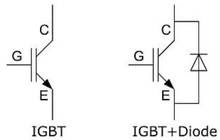
\includegraphics[width=0.85\linewidth]{images/IGBT.png}
\end{center}

\subsubsection{Tail-Strom und Abschaltverluste}

Beim Abschalten verbleibt Speicherladung im Driftgebiet.

Tail-Strom:
\[
i_{tail}(t)
\]

Zusätzliche Verluste:
\[
\boxed{P_{off} \gg P_{on}}
\]

Konsequenz:
\begin{itemize}
\item langsamer als MOSFET,
\item dafür geringere Leitverluste bei grossen Strömen.
\end{itemize}

\subsection{Vergleich der Bauelemente}

\begin{center}
\begin{tabular}{l|c|c|c|c}
 & Diode & Thyristor & MOSFET & IGBT \\
\hline
Steuerbar & nein & Zünden & ja & ja \\
Abschaltbar & ja & nein & ja & ja \\
Schaltfreq. & mittel & tief & sehr hoch & mittel \\
Leitverluste & klein & klein & klein bei klein $I$ & klein bei gross $I$ \\
Speicherladung & ja & ja & nein & ja \\
\end{tabular}
\end{center}
\subsection{Safe Operating Area (SOA)}

Die Safe Operating Area beschreibt den zulässigen Arbeitsbereich eines Leistungshalbleiters
im Strom–Spannungs–Diagramm.

Zulässige Grenzbedingungen:
\[
\boxed{
\begin{aligned}
u &< U_{RRM} \\
i &< I_{\max} \\
P &= u \cdot i < P_{\max} \\
\frac{di}{dt} &< \left(\frac{di}{dt}\right)_{\max} \\
\frac{du}{dt} &< \left(\frac{du}{dt}\right)_{\max}
\end{aligned}
}
\]

Physikalische Bedeutung:
\begin{itemize}
\item Begrenzung durch Durchbruchspannung,
\item Begrenzung durch thermische Überlast,
\item Begrenzung durch sekundären Durchbruch (bipolare Bauelemente).
\end{itemize}

Die Einhaltung der SOA ist zwingend für den sicheren Betrieb.


\subsection{Zusammenfassung der Verlustmechanismen}

Gesamtverluste:
\[
\boxed{P_V = P_{cond} + P_{sw}}
\]

mit:
\[
P_{cond} = U_0 I_{\mathrm{avg}} + r I_{\mathrm{RMS}}^2
\]
\[
P_{sw} = f_s \int u(t)i(t)\,dt
\]

Thermische Auslegung:
\[
T_j = T_{amb} + R_{th} P_V < T_{j,\max}.
\]
\subsection{Vereinfachte Schaltverlustrechnung}

Bei näherungsweise linearem Spannungs- und Stromverlauf während des Schaltens gilt:

\paragraph{Einschaltverlust}

\[
\boxed{E_{on} \approx \frac{1}{2} U \, I \, t_{on}}
\]

\paragraph{Ausschaltverlust}

\[
\boxed{E_{off} \approx \frac{1}{2} U \, I \, t_{off}}
\]

Mittlere Schaltverluste:

\[
\boxed{
P_{sw} = f_s \left(E_{on} + E_{off}\right)
}
\]

Konsequenzen:
\begin{itemize}
\item $f_s \uparrow \Rightarrow P_{sw} \uparrow$
\item $t_{on}, t_{off}$ klein $\Rightarrow$ geringe Verluste.
\end{itemize}

\subsection{Thermische Widerstandskette}

\[
\boxed{R_{th,tot} = R_{th,jc} + R_{th,ck} + R_{th,ka}}
\]

Temperaturen:

\[
T_j = T_{amb} + R_{th,tot} P_V
\]
\[
T_c = T_j - R_{th,jc} P_V,
\qquad
T_k = T_c - R_{th,ck} P_V
\]

Grenzbedingung:
\[
\boxed{T_j < T_{j,\max}}
\]
\subsection{Vereinfachte Schaltverlustrechnung}

Bei näherungsweise linearem Spannungs- und Stromverlauf während des Schaltens gilt:

\paragraph{Einschaltverlust}

\[
\boxed{E_{on} \approx \frac{1}{2} U \, I \, t_{on}}
\]

\paragraph{Ausschaltverlust}

\[
\boxed{E_{off} \approx \frac{1}{2} U \, I \, t_{off}}
\]

Mittlere Schaltverluste:

\[
\boxed{
P_{sw} = f_s \left(E_{on} + E_{off}\right)
}
\]

Konsequenzen:
\begin{itemize}
\item $f_s \uparrow \Rightarrow P_{sw} \uparrow$
\item $t_{on}, t_{off}$ klein $\Rightarrow$ geringe Verluste.
\end{itemize}

        \input{sections/01_Zeitbereichanalse_R_L_Lasten.tex}
        \section{Mittelwert, Effektivwert und Leistung}

Diese Section behandelt die \textbf{zentralen Bewertungsgrössen} für periodische, nichtsinusförmige Spannungen und Ströme,
wie sie in Gleichrichtern, Stellern und Wechselrichtern auftreten.

\smallskip

\textbf{Zielbild:}
\begin{itemize}
    \item Definition von Mittelwert und Effektivwert
    \item Physikalische Interpretation (DC-Anteil, thermische Wirkung)
    \item Leistungsberechnung bei allgemeinen periodischen Signalen
    \item Anwendung auf stückweise definierte Zeitverläufe aus Übungen
\end{itemize}

\subsection{Periodische Signale und Grundbegriffe}

Ein Signal $x(t)$ heisst \textbf{periodisch} mit Periodendauer $T$, wenn gilt:
\[
x(t) = x(t+T) \qquad \forall t.
\]

Typische Beispiele aus der Leistungselektronik:
\begin{itemize}
    \item Gleichgerichtete Sinusspannung (Halb- und Vollwelle)
    \item Strom im R-L-Kreis bei Schaltbetrieb
    \item PWM-Ausgangsspannungen
\end{itemize}

\crd{\textrightarrow\ Mittelwert und Effektivwert werden immer über \textbf{eine volle Periode $T$} gebildet.}

\subsection{Zeitmittelwert (Gleichwert, DC-Anteil)}

\subsubsection{Definition}

Der \textbf{Zeitmittelwert} (Mittelwert) eines periodischen Signals $x(t)$ ist definiert als:
\[
\cbl{\overline{x} = \frac{1}{T} \int_{0}^{T} x(t)\,\diff t.}
\]

Interpretation:
\begin{itemize}
    \item Entspricht dem \textbf{Gleichanteil} des Signals.
    \item Bei Strom: mittlerer Transport von Ladung pro Zeit.
    \item Bei Spannung: DC-Anteil der Ausgangsspannung eines Gleichrichters.
\end{itemize}

\subsubsection{Typische Eigenschaften}

\begin{itemize}
    \item Symmetrische Wechselgrössen: $\overline{x}=0$.
    \item Gleichgerichtete Signale: $\overline{x}>0$.
    \item Für stückweise definierte Signale:
    \[
    \overline{x} = \frac{1}{T} \left( \int_{t_1}^{t_2} x_1(t)\,\diff t + \int_{t_2}^{t_3} x_2(t)\,\diff t + \dots \right).
    \]
\end{itemize}

\crd{\textrightarrow\ Mittelwert ist \textbf{nicht} gleich Effektivwert. Häufige Prüfungsfalle.}

\subsection{Effektivwert (RMS)}

\subsubsection{Definition}

Der \textbf{Effektivwert} eines periodischen Signals $x(t)$ ist definiert als:
\[
\cbl{x_{\mathrm{RMS}} = \sqrt{\frac{1}{T} \int_{0}^{T} x^2(t)\,\diff t}.}
\]

Interpretation:
\begin{itemize}
    \item Entspricht dem \textbf{Gleichwert}, der in einem Widerstand \textbf{die gleiche Verlustleistung} erzeugt.
    \item Thermische Wirkung.
    \item Grundlage für Dimensionierung von Leitern, Bauteilen und Verlusten.
\end{itemize}

\subsubsection{Vergleich Mittelwert vs. Effektivwert}

\begin{itemize}
    \item Mittelwert: lineare Mittelung.
    \item Effektivwert: quadratische Mittelung.
    \item Allgemein gilt:
    \[
    x_{\mathrm{RMS}} \ge |\overline{x}|.
    \]
\end{itemize}

\subsection{Momentanleistung und Wirkleistung}

\subsubsection{Momentanleistung}

Für allgemeine Spannungen und Ströme:
\[
\cbl{p(t) = u(t)\, i(t).}
\]

Diese Grösse schwankt zeitlich, auch im stationären Betrieb.

\subsubsection{Wirkleistung}

Die \textbf{mittlere Wirkleistung} ist definiert als:
\[
\cbl{P = \overline{p(t)} = \frac{1}{T} \int_{0}^{T} u(t)\,i(t)\,\diff t.}
\]

\subsubsection{Spezialfall: Ohmsche Last}

Für $u(t) = R\, i(t)$ gilt:
\[
\cbl{P = R \, I_{\mathrm{RMS}}^2 = \frac{U_{\mathrm{RMS}}^2}{R}.}
\]

Interpretation:
\begin{itemize}
    \item Nur der Effektivwert bestimmt die Verlustleistung.
    \item Unabhängig von der Signalform.
\end{itemize}

\subsection{Berechnung bei stückweise definierten Signalen}

In vielen Übungen ist $x(t)$ stückweise gegeben:
\[
x(t) =
\begin{cases}
x_1(t), & 0 < t < T_1,\\
x_2(t), & T_1 < t < T_2,\\
\dots
\end{cases}
\]

Dann gilt:

\paragraph{Mittelwert}
\[
\cbl{\overline{x} = \frac{1}{T} \sum_k \int_{T_k} x_k(t)\,\diff t.}
\]

\paragraph{Effektivwert}
\[
\cbl{x_{\mathrm{RMS}} = \sqrt{ \frac{1}{T} \sum_k \int_{T_k} x_k^2(t)\,\diff t }.}
\]

\paragraph{Wirkleistung}
\[
\cbl{P = \frac{1}{T} \sum_k \int_{T_k} u_k(t)\, i_k(t)\,\diff t.}
\]

\crd{\textrightarrow\ Bei stückweisen Verläufen immer korrekt die Zeitintervalle trennen.}

\subsection{Bezug zu Fourier-Reihen}

Für ein periodisches Signal mit Fourierkoeffizienten gilt (Parseval):

\[
\cbl{X_{\mathrm{RMS}}^2 = \frac{a_0^2}{2} + \sum_{n=1}^\infty \left( a_n^2 + b_n^2 \right).}
\]

Interpretation:
\begin{itemize}
    \item Effektivwert ist die Summe der Quadrate aller Harmonischen.
    \item Harmonische tragen direkt zur Verlustleistung bei.
\end{itemize}

\subsection{Skizze 1: Nichtsinusförmiger periodischer Strom}

\begin{center}
\begin{tikzpicture}[scale=1]
\draw[->] (0,0) -- (8,0) node[right] {$t$};
\draw[->] (0,0) -- (0,3) node[above] {$i(t)$};

\draw (0,1) -- (2,2.5) -- (4,1) -- (6,2.5) -- (8,1);

\draw[dashed] (0,1) -- (8,1) node[right] {$\overline{i}$};
\draw[dashed] (0,2) -- (8,2) node[right] {$i_{\mathrm{RMS}}$};

\draw (4,0) node[below] {$T/2$};
\draw (8,0) node[below] {$T$};
\end{tikzpicture}
\end{center}

\textbf{Aussage:}
\begin{itemize}
    \item Mittelwert ist die horizontale Mittel-Linie.
    \item Effektivwert liegt darüber.
\end{itemize}

\subsection{Skizze 2: Quadratbildung für Effektivwert}

\begin{center}
\begin{tikzpicture}[scale=1]
\draw[->] (0,0) -- (8,0) node[right] {$t$};
\draw[->] (0,0) -- (0,3) node[above] {$x^2(t)$};

\draw (0,0.5) -- (2,2.5) -- (4,0.5) -- (6,2.5) -- (8,0.5);

\draw[dashed] (0,1.5) -- (8,1.5) node[right] {$\overline{x^2}$};
\end{tikzpicture}
\end{center}

\textbf{Aussage:}
\begin{itemize}
    \item Zuerst quadrieren.
    \item Dann mitteln.
    \item Dann Wurzel ziehen.
\end{itemize}

\subsection{Skizze 3: Leistung bei ohmscher Last}

\begin{center}
\begin{tikzpicture}[scale=1]
\draw[->] (0,0) -- (8,0) node[right] {$t$};
\draw[->] (0,0) -- (0,3) node[above] {$p(t)$};

\draw (0,1.5) .. controls (1,2.5) .. (2,1.5)
      .. controls (3,0.5) .. (4,1.5)
      .. controls (5,2.5) .. (6,1.5)
      .. controls (7,0.5) .. (8,1.5);

\draw[dashed] (0,1.5) -- (8,1.5) node[right] {$P$};
\end{tikzpicture}
\end{center}

\textbf{Aussage:}
\begin{itemize}
    \item Momentanleistung schwankt.
    \item Wirkleistung ist der Mittelwert.
\end{itemize}

\subsection{Typische Fehlerquellen}

\begin{itemize}
    \item Mittelwert mit Effektivwert verwechselt.
    \item Quadrat beim RMS vergessen.
    \item Falsche Periodendauer $T$ eingesetzt.
    \item Stückweise Integrale nicht getrennt.
    \item Leistung mit $U_{\mathrm{RMS}}\cdot I_{\mathrm{RMS}}$ berechnet bei nichtohmscher Last.
\end{itemize}

\subsection{Minimal-Checkliste für Aufgaben}

\begin{enumerate}
    \item Periodendauer $T$ bestimmen.
    \item Signalform stückweise festlegen.
    \item Mittelwert berechnen.
    \item Effektivwert berechnen.
    \item Bei Leistung: $p(t)=u(t)i(t)$ bilden und mitteln.
    \item Plausibilität prüfen: $x_{\mathrm{RMS}} \ge |\overline{x}|$.
\end{enumerate}

        \section{Buck-, Boost- und Buck-Boost-Converter}
DC-DC-Wandler sind spezielle Gleichstromsteller
Diese Section behandelt die wichtigsten nichtisolierten Gleichstromsteller zur
Spannungsanpassung in DC-Systemen.  
Sie unterscheiden sich von den klassischen Gleichstromstellern durch ihre
spezifische Topologie und ihren kontinuierlichen Energietransfer über eine Induktivität.

\smallskip
\paragraph{Grenzinduktivität für kontinuierlichen Betrieb}
\[
L_{\min} = \frac{(1-d)R}{2 f_s}
\]


\textbf{Zielbild:}
\begin{itemize}
    \item Grundprinzip der drei wichtigsten DC-DC-Wandler verstehen
    \item Mittelwertzusammenhänge kennen
    \item Einordnung zu Gleichstromstellern beherrschen
\end{itemize}

% -------------------------------------------------
\subsection{Allgemeines Grundprinzip}

Alle DC-DC-Wandler arbeiten mit:

\begin{itemize}
    \item Schalter
    \item Diode (oder synchroner Schalter)
    \item Induktivität $L$
    \item Glättkondensator $C$
\end{itemize}

Grundgleichung (idealer Fall, stationär):

\[
\cbl{u_L = L \frac{di_L}{dt}}
\qquad
\Rightarrow
\qquad
\cbl{\overline{u_L} = 0}
\]

\crd{\textrightarrow\ Im stationären Zustand ist der Mittelwert der Induktionsspannung null.}

% -------------------------------------------------
\subsection{Buck-Converter (Abwärtssteller)}

% --- HIER: bestehende oder spätere Grafik Buck ---
Buck-Converter (Abwärtssteller):
\begin{center}

    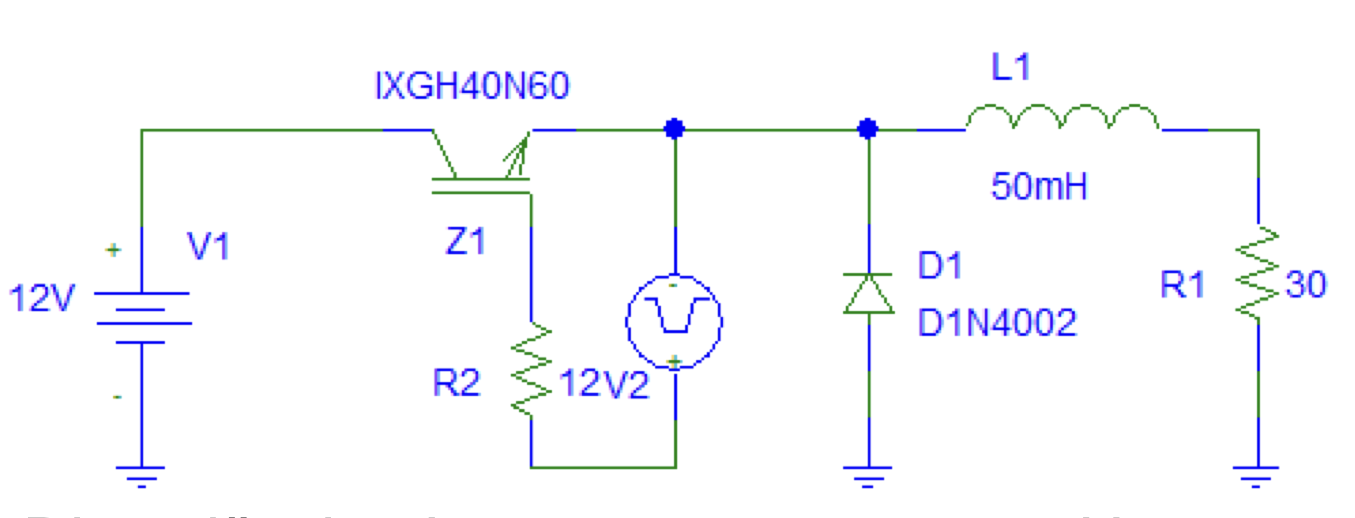
\includegraphics[width=0.85\linewidth]{images/Buckconverter.png}

\end{center}
Zeitverlauf Buck-Converter:
\begin{center}
    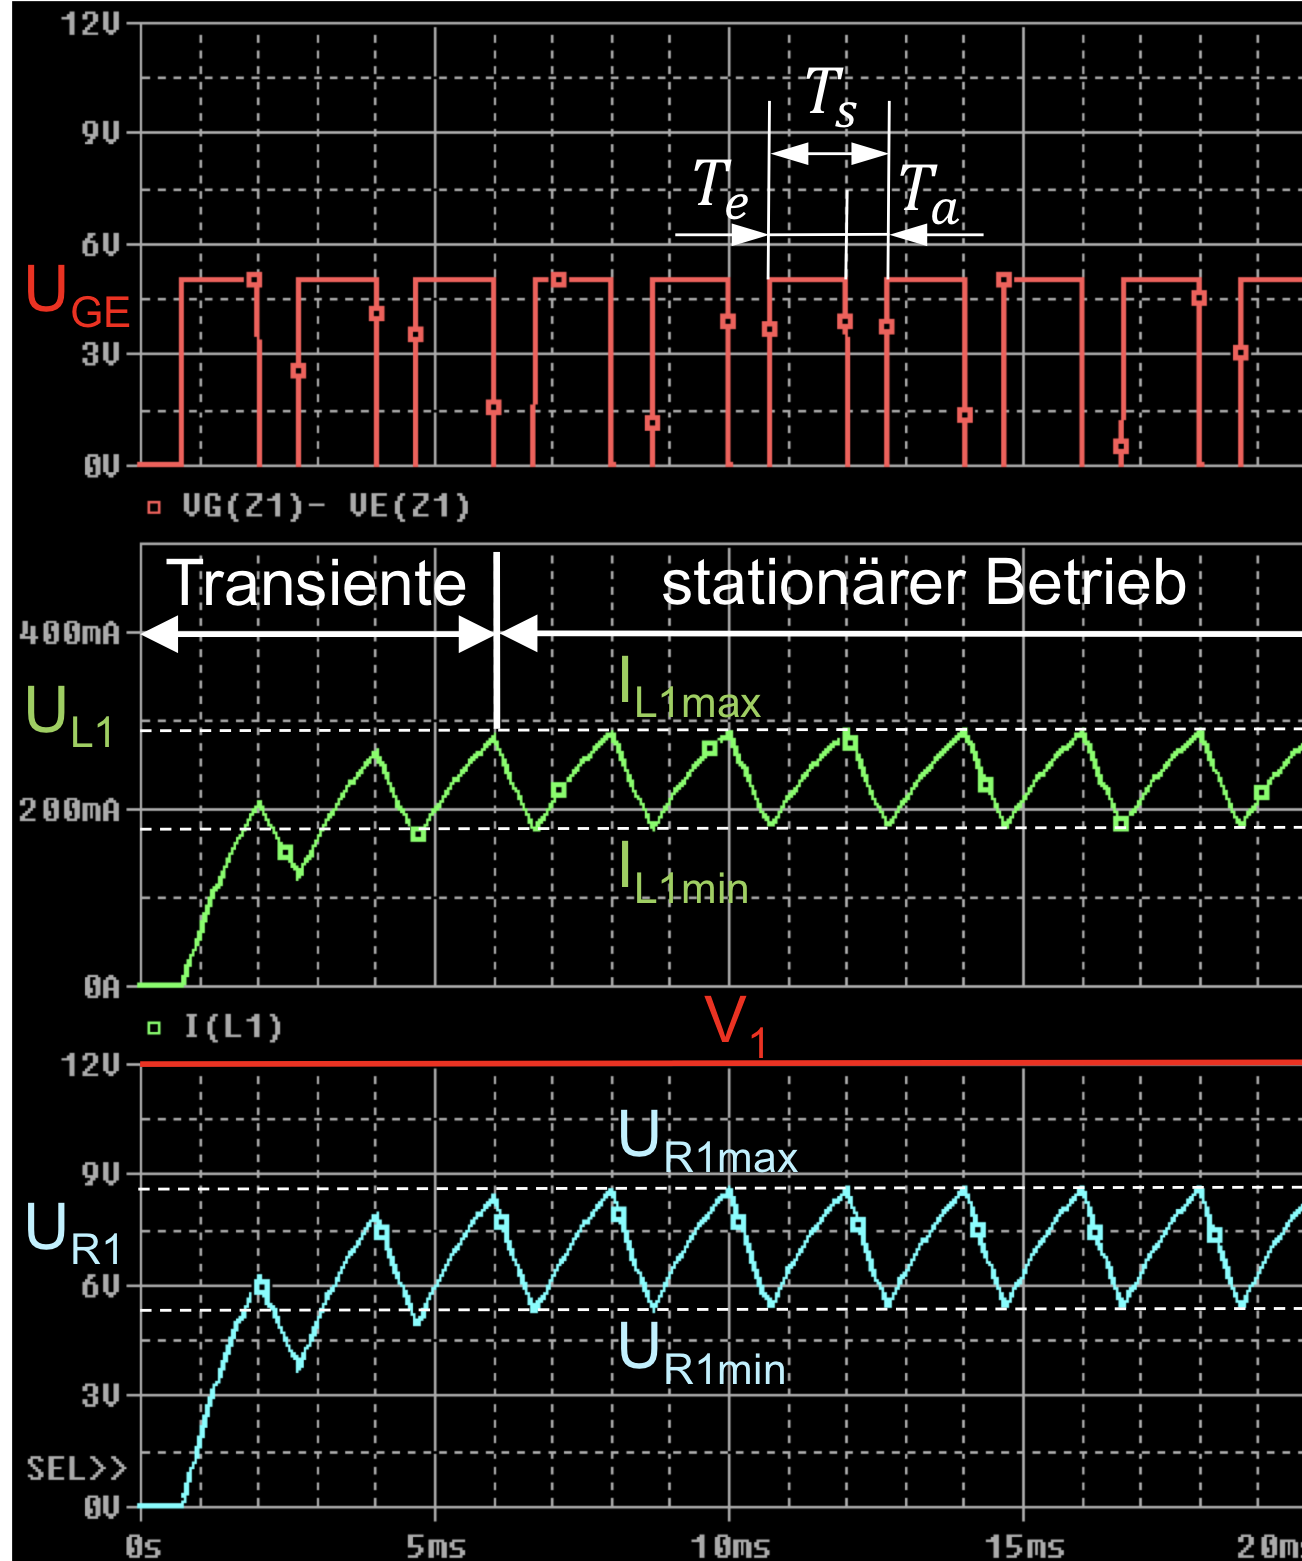
\includegraphics[width=0.85\linewidth]{images/Buckconverter_verlauf.png}
\end{center}
Ziel:
\[
u_2 < U_{DC}
\]

Mittelwert:
\[
\cbl{u_2 = d \, U_{DC}}
\]

Für $L < L_{\min}$ geht der Betrieb in den diskontinuierlichen Modus über.
Dann gelten die Mittelwertformeln nicht mehr exakt.

Eigenschaften:
\begin{itemize}
    \item Ausgangsspannung kleiner als Eingang
    \item Kontinuierlicher Ausgangsstrom
    \item Standardwandler in Netzteilen
\end{itemize}

% -------------------------------------------------
\subsection{Boost-Converter (Aufwärtssteller)}

% --- HIER: bestehende oder spätere Grafik Boost ---
\begin{center}
    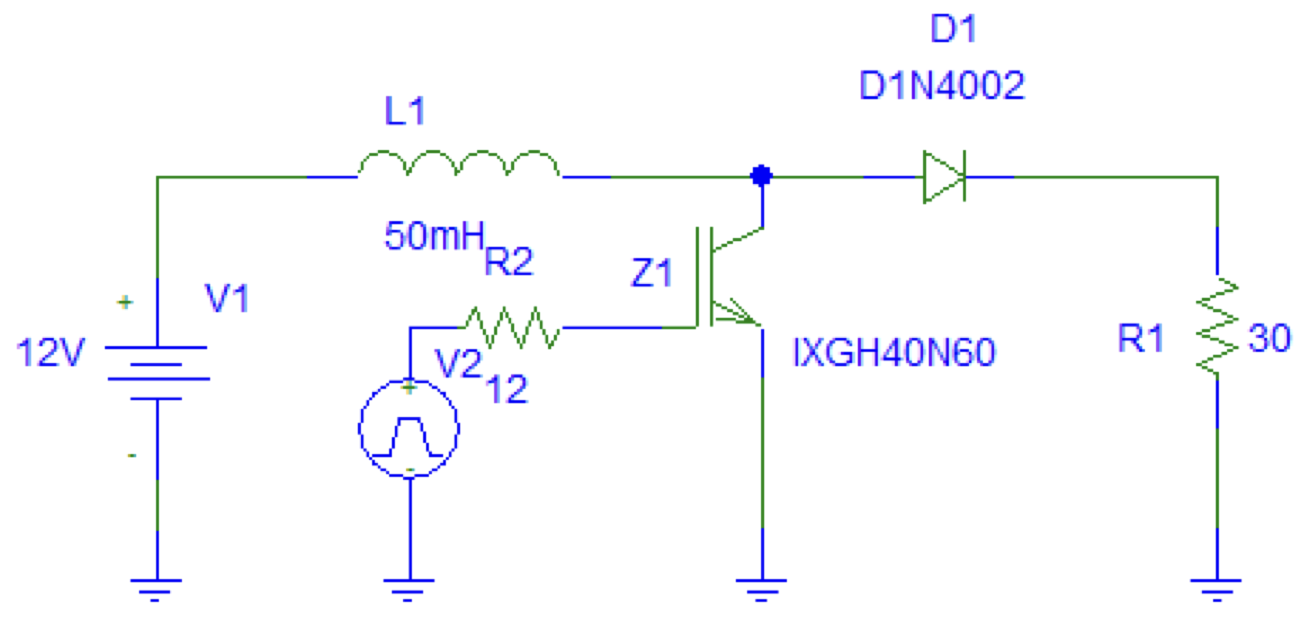
\includegraphics[width=0.85\linewidth]{images/Boostconv.png}
\end{center}
Zeitverlauf Boost-Converter:
\begin{center}
    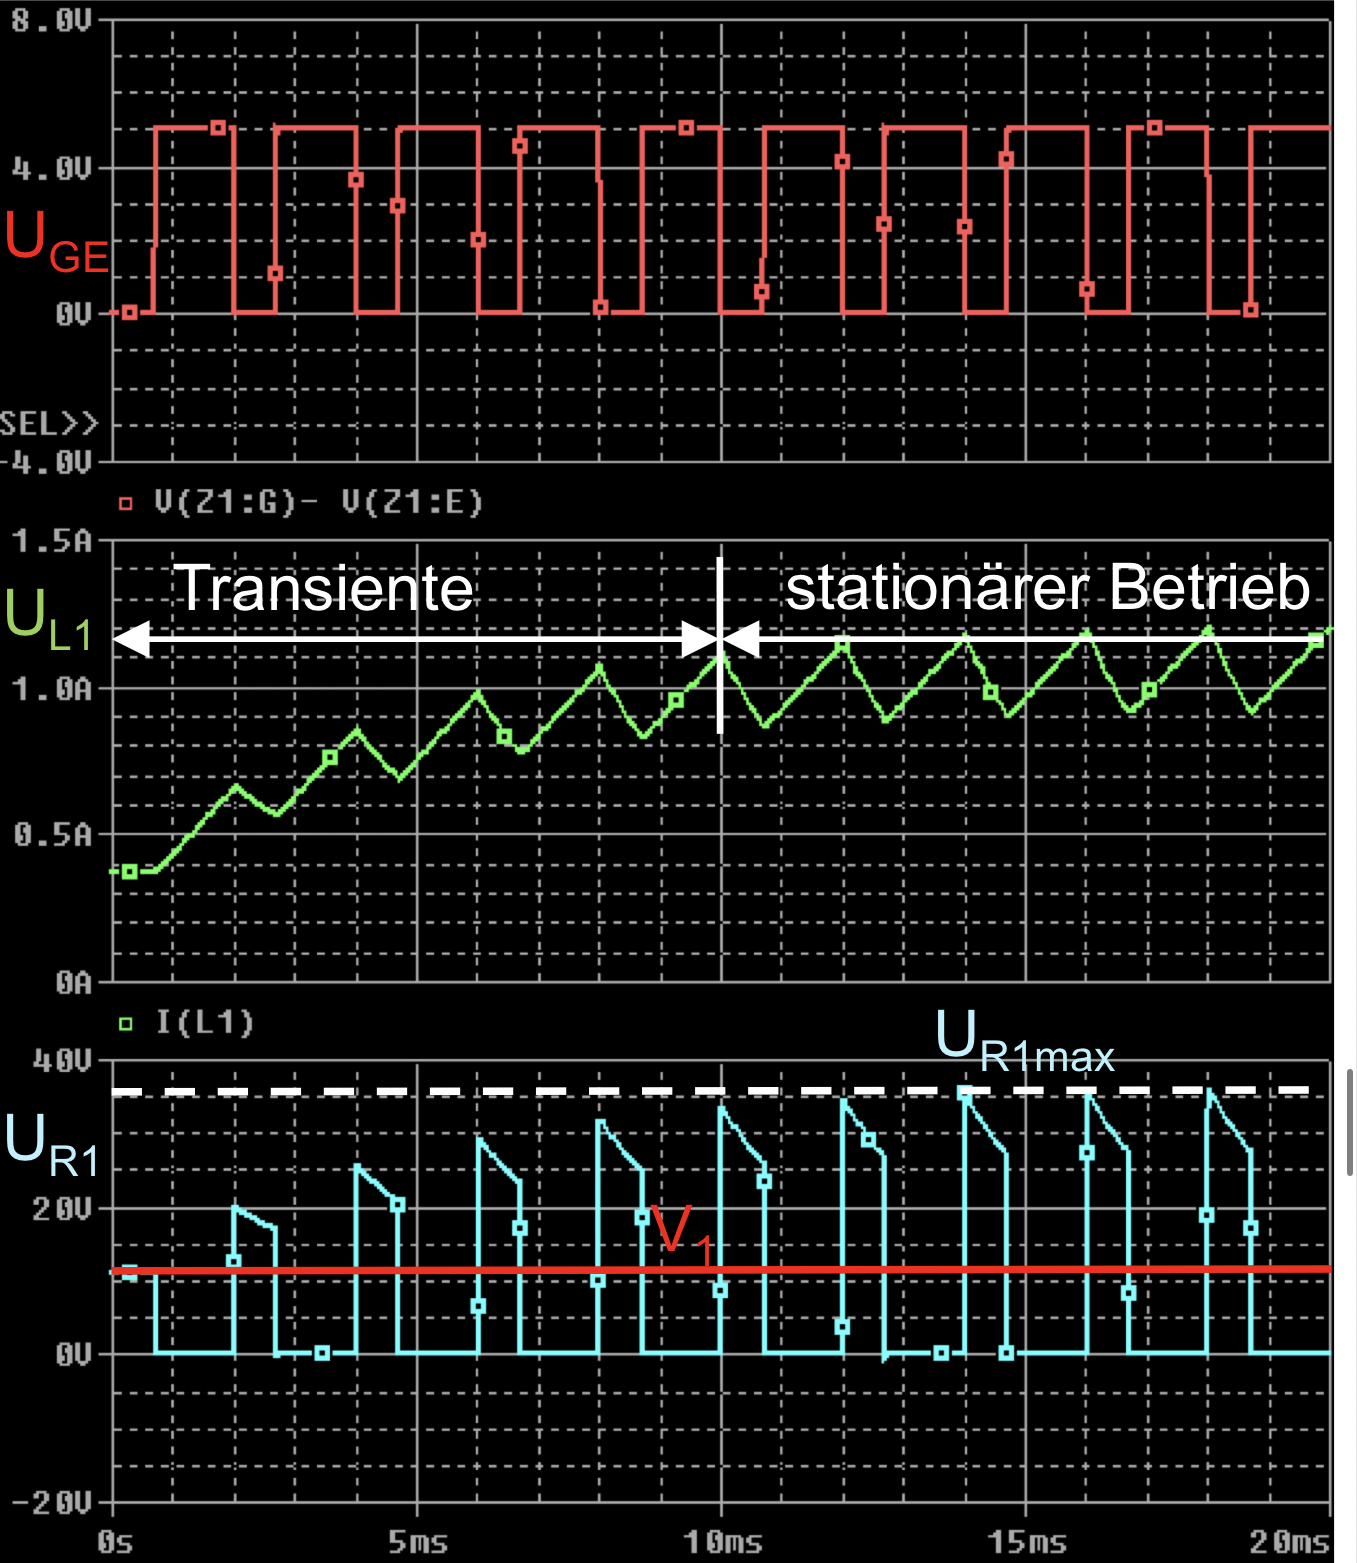
\includegraphics[width=0.85\linewidth]{images/Boostconv_verlauf.png}
\end{center}

Ziel:
\[
u_2 > U_{DC}
\]

Mittelwert:
\[
\cbl{u_2 = \frac{U_{DC}}{1-d}}
\]

Eigenschaften:
\begin{itemize}
    \item Ausgangsspannung grösser als Eingang
    \item Eingangsstrom gepulst
\end{itemize}

% -------------------------------------------------
\subsection{Buck-Boost-Converter}

% --- HIER: bestehende oder spätere Grafik Buck-Boost ---
\begin{center}
    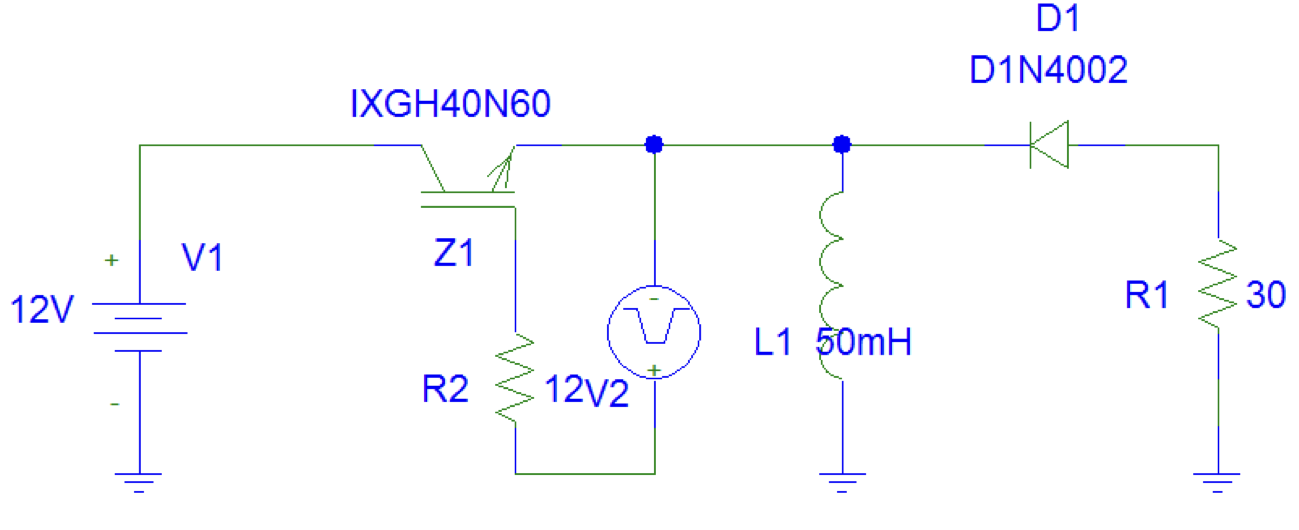
\includegraphics[width=0.85\linewidth]{images/Buckboostconv.png}
\end{center}
Zeitverlauf Buck-Boost-Converter:
\begin{center}
    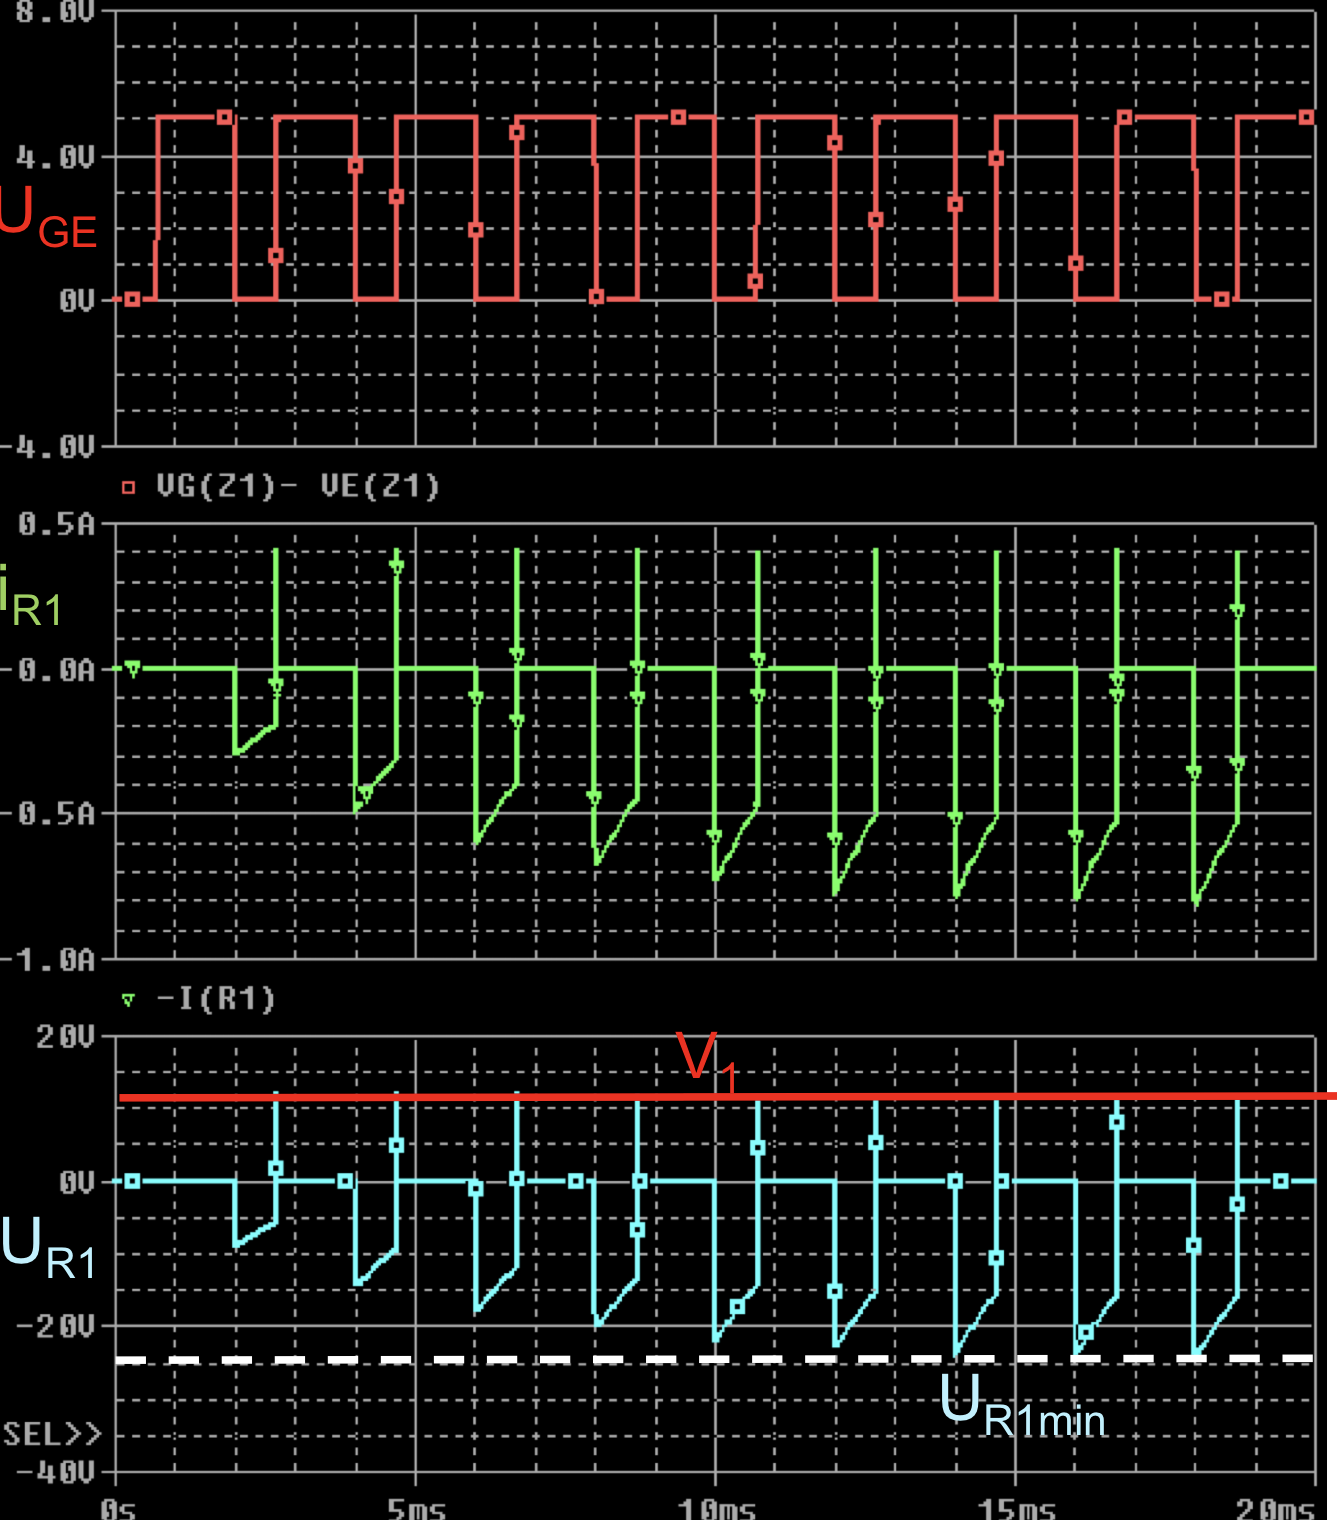
\includegraphics[width=0.85\linewidth]{images/Buckboostconv_verlauf.png}
\end{center}


Ziel:
\[
u_2 < 0 \quad \text{oder} \quad |u_2| > U_{DC}
\]

Mittelwert:
\[
\cbl{u_2 = -\frac{d}{1-d} U_{DC}}
\]
\paragraph{Stromrippel im Buck-Converter}
Im kontinuierlichen Betrieb gilt näherungsweise:
\[
\Delta i_L = \frac{(U_{DC} - u_2)}{L} \, d T_s
\]

Eigenschaften:
\begin{itemize}
    \item Polaritätsumkehr
    \item Spannung grösser oder kleiner als Eingang möglich
\end{itemize}

% -------------------------------------------------
\subsection{Vergleich der DC-DC-Wandler}

\begin{center}
\begin{tabular}{l|c|c|c}
 & Buck & Boost & Buck-Boost \\ \hline
$u_2/U_{DC}$ & $d$ & $\frac{1}{1-d}$ & $-\frac{d}{1-d}$ \\
Polarität & gleich & gleich & \cbl{invertiert} \\
$u_2<U_{DC}$ & \cbl{ja} & nein & ja \\
$u_2>U_{DC}$ & nein & \cbl{ja} & ja \\
\end{tabular}
\end{center}

\subsection{Abgrenzung zu klassischen Gleichstromstellern}

\begin{itemize}
    \item Klassischer Gleichstromsteller: direkte Pulsweitensteuerung der Last.
    \item DC-DC-Wandler: Energieübertragung über Induktivität mit Spannungsanpassung.
\end{itemize}

\crd{\textrightarrow\ Buck/Boost sind spezielle Gleichstromsteller mit Energiespeicher.}

        \section{Systematik der Gleichrichterbezeichnungen}

Die Bezeichnungen der Gleichrichter folgen einer einheitlichen Nomenklatur:

\begin{itemize}
\item M = Mittelpunktschaltung
\item B = Brückenschaltung
\item Zahl = Pulszahl pro Netzperiode
\item U = ungesteuert (Dioden)
\item C = gesteuert (Thyristoren)
\end{itemize}

\subsection{Bedeutung der Kennzeichnung}

\begin{center}
\begin{tabular}{l|l}
Bezeichnung & Bedeutung \\ \hline
M1U & Einpuls, Mittelpunkt, ungesteuert \\
M1C & Einpuls, Mittelpunkt, gesteuert \\
B2U & Zweipuls, Brücke, ungesteuert \\
B2C & Zweipuls, Brücke, gesteuert \\
B6U & Sechspuls, Brücke, ungesteuert \\
B6C & Sechspuls, Brücke, gesteuert \\
\end{tabular}
\end{center}

\subsection{Grundklassifikation}

\begin{itemize}
\item Ungesteuerte Gleichrichter (U): Dioden, keine Stellmöglichkeit.
\item Gesteuerte Gleichrichter (C): Thyristoren, Stellgrösse Zündwinkel $\alpha$.
\item Pulszahl bestimmt die Restwelligkeit der Gleichspannung.
\end{itemize}

\crd{\textrightarrow\ Diese Systematik gilt für alle folgenden Gleichrichterkapitel.}

        \section{Einpuls-Gleichrichter}

\subsection{M1U: Ungesteuerter Einpuls-Gleichrichter}

% --- bestehende Grafik: Schaltung ---
Einpuls-Gleichrichter M1U
\begin{center}
    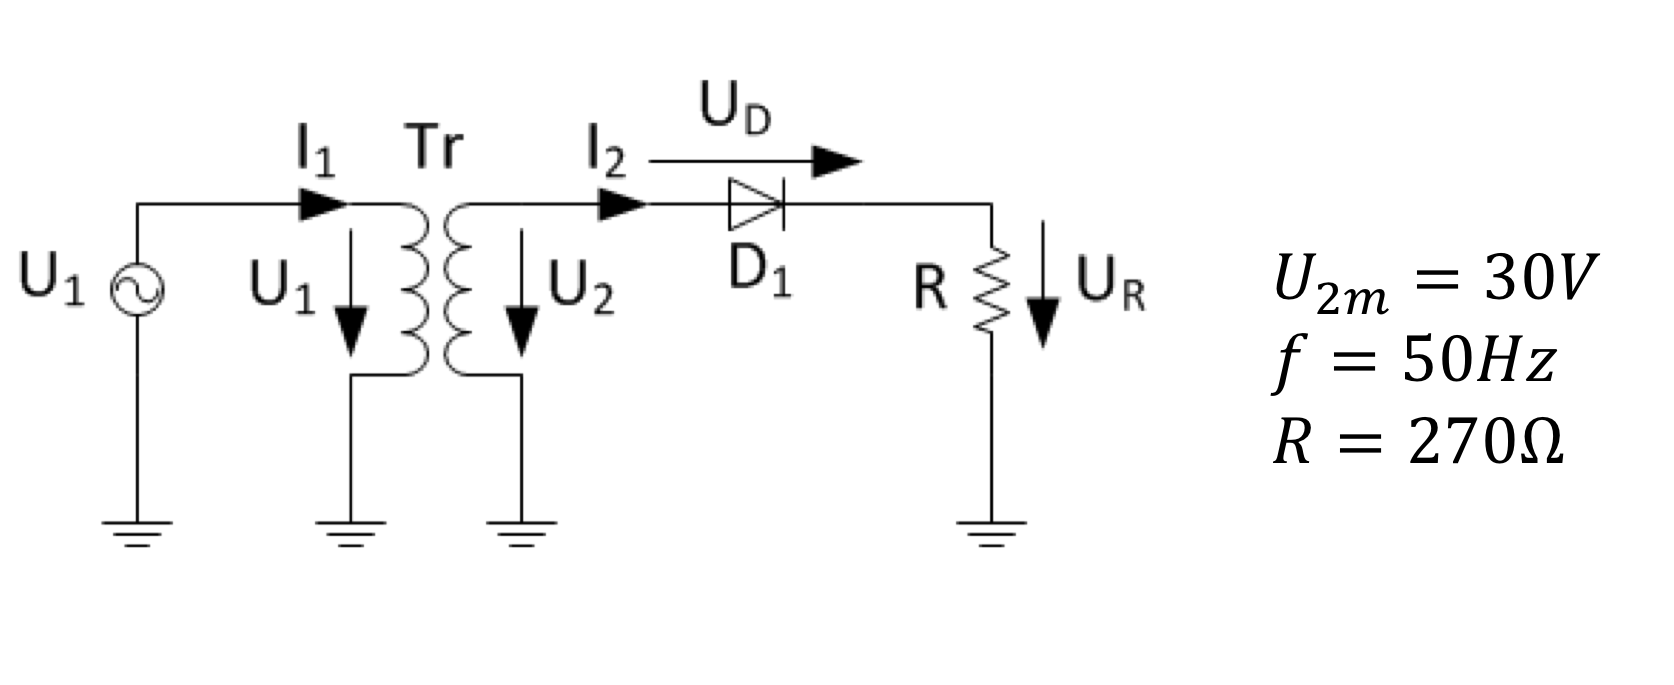
\includegraphics[width=0.85\linewidth]{images/M1U.png}
\end{center}

Der ungesteuerte Einpuls-Gleichrichter besteht aus einer Diode und einer Wechselspannungsquelle.
Er liefert eine pulsierende Gleichspannung mit einer Pulszahl von $p=1$.

Momentane Ausgangsspannung:
\[
u_d(t) =
\begin{cases}
u_s(t), & u_s(t) \ge 0 \\
0, & u_s(t) < 0
\end{cases}
\]

Mittelwert:
\[
\cbl{\overline{u_d} = \frac{\hat U}{\pi}}
\]

Effektivwert:
\[
\cbl{U_{d,\mathrm{RMS}} = \frac{\hat U}{2}}
\]

Eigenschaften:
\begin{itemize}
    \item Keine Stellmöglichkeit
    \item Starke Welligkeit der Gleichspannung
    \item Einfachste Gleichrichterschaltung
\end{itemize}

% --- bestehende Grafik: Spannungsverlauf ---
\begin{center}

    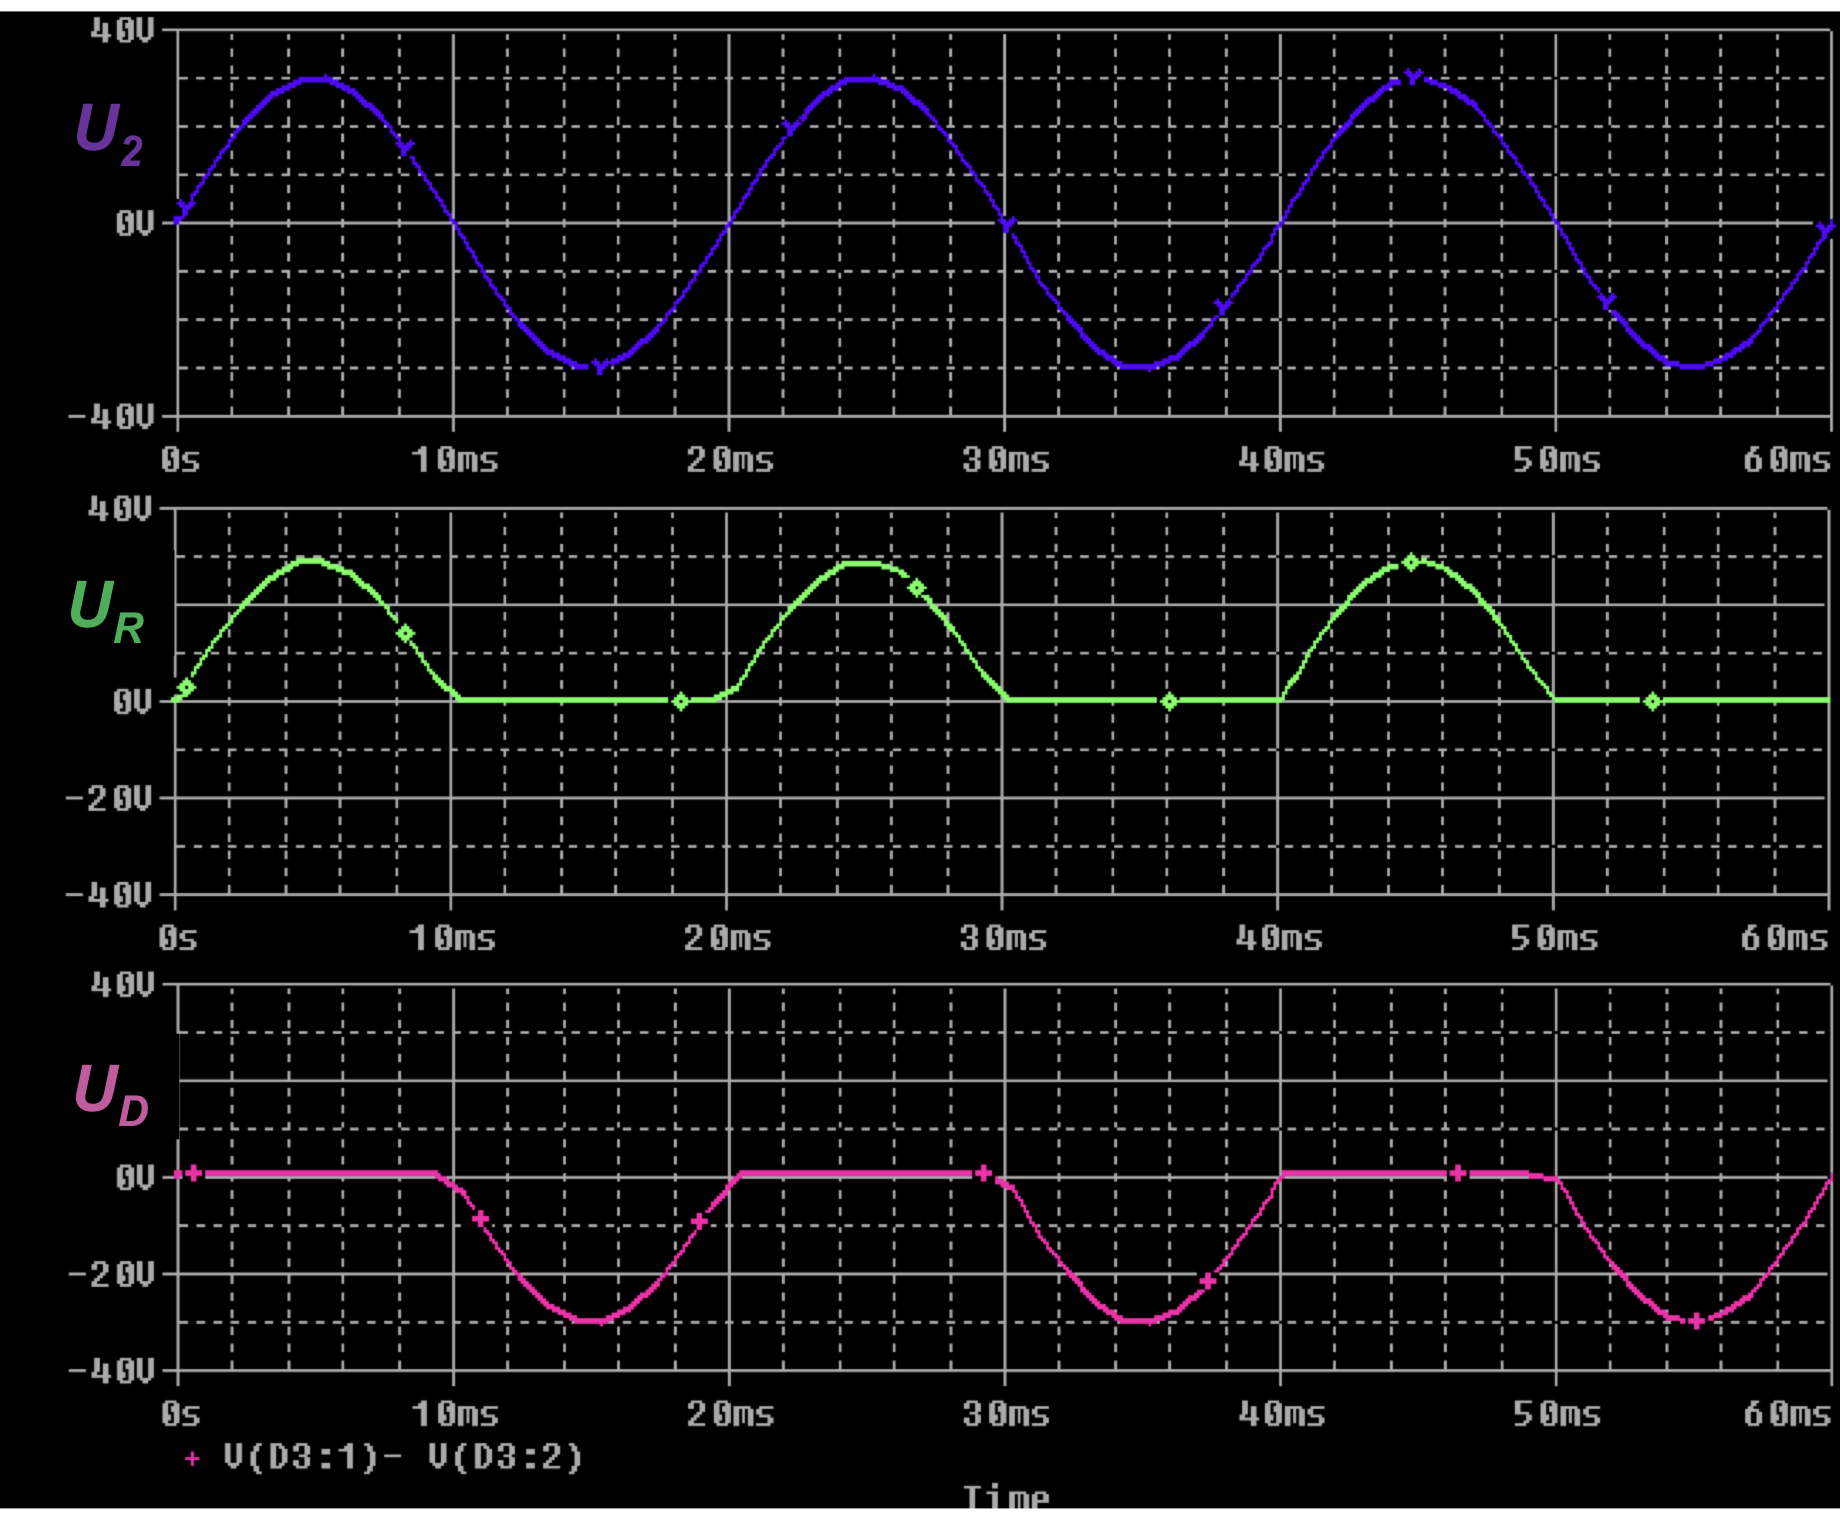
\includegraphics[width=0.85\linewidth]{images/M1U_verlauf.png}

\end{center}
Ausgangsspannung $u_d(t)$ beim M1U
% -------------------------------------------------
\subsection{M1U mit kapazitiver Last}

Bei kapazitiver Last leitet die Diode nur während eines kurzen Intervalls um das Spannungsmaximum.
Zwischen zwei Leitphasen entlädt sich der Kondensator über den Widerstand.

\paragraph{Sperrphase der Diode}

Für die Sperrphase gilt die Differentialgleichung:

\[
\frac{u_R(t)}{R} + C \frac{du_R(t)}{dt} = 0
\]

mit der Zeitkonstante:

\[
\cbl{\tau = RC}
\]

Lösung der Differentialgleichung:

\[
\cbl{u_R(t) = B \, e^{-t/\tau}}
\]

\paragraph{Ausschaltwinkel}

Der Ausschaltwinkel $\beta_a$ ergibt sich aus:

\[
\cbl{\tan \beta_a = - \omega \tau}
\]

\paragraph{Einschaltwinkel}

Der Einschaltwinkel $\beta_e$ folgt aus der Bedingung:

\[
\cbl{U_{2m} \sin \beta_e = U_{2m} \sin \beta_a \, e^{(\beta_a - \beta_e)/(\omega \tau)}}
\]

Dies ist eine transzendente Gleichung und wird numerisch oder grafisch gelöst.

\crd{\textrightarrow\ Diese Methode wird direkt in Prüfungen für M1U mit C-Last verwendet.}

\subsection{M1C: Gesteuerter Einpuls-Gleichrichter}

% --- bestehende oder neue Grafik: Thyristor-Schaltung ---
Gesteuerter Einpuls-Gleichrichter M1C
\begin{center}
    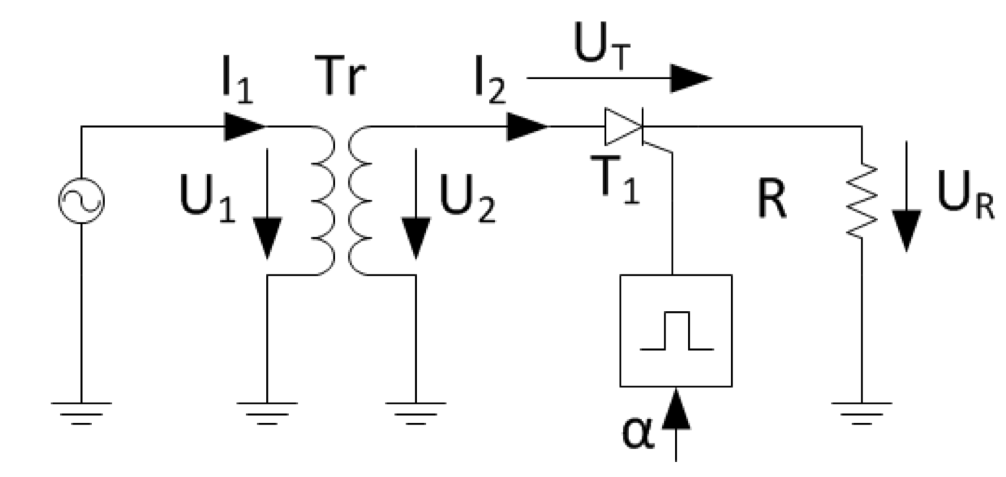
\includegraphics[width=0.85\linewidth]{images/M1C.png}
\end{center}

Beim gesteuerten Einpuls-Gleichrichter wird die Diode durch einen Thyristor ersetzt.
Die Gleichspannung ist über den Zündwinkel $\alpha$ steuerbar.

Momentane Ausgangsspannung:
\[
u_d(t) =
\begin{cases}
u_s(t), & \omega t \ge \alpha \\
0, & \omega t < \alpha
\end{cases}
\]

Mittelwert:
\[
\cbl{\overline{u_d} = \frac{\hat U}{2\pi}(1+\cos\alpha)}
\]

Eigenschaften:
\begin{itemize}
    \item Stellbereich: $0 \le \alpha \le \pi$
    \item Bei $\alpha = 0$: maximaler Mittelwert
    \item Bei $\alpha = \pi$: $\overline{u_d} = 0$
\end{itemize}

\crd{\textrightarrow\ M1C ist der einfachste gesteuerte Gleichrichter.}

        \section{Zweipuls-Gleichrichter}

\subsection{B2U: Ungesteuerter Zweipuls-Gleichrichter}

% --- bestehende Grafik: Brückenschaltung ---
\begin{figure}[h]
\centering
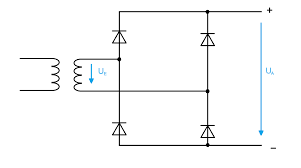
\includegraphics[width=0.6\linewidth]{images/B2U.png}
\caption{Zweipuls-Brückengleichrichter B2U}
\end{figure}

Der B2U-Gleichrichter ist eine vollwellige Brückenschaltung mit vier Dioden.
Die Pulszahl beträgt $p=2$.

Momentane Ausgangsspannung:
\[
u_d(t) = |u_s(t)|
\]

Mittelwert:
\[
\cbl{\overline{u_d} = \frac{2\hat U}{\pi}}
\]

Effektivwert:
\[
\cbl{U_{d,\mathrm{RMS}} = \frac{\hat U}{\sqrt{2}}}
\]

Eigenschaften:
\begin{itemize}
    \item Keine Stellmöglichkeit
    \item Geringere Welligkeit als M1U
    \item Standard-Gleichrichtertopologie
\end{itemize}

% --- bestehende Grafik: Spannungsverlauf ---
\begin{center}
    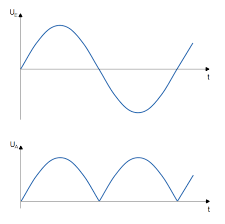
\includegraphics[width=0.85\linewidth]{images/B2U_verlauf.png}
\end{center}
        \subsection{B2C: Gesteuerter Zweipuls-Gleichrichter}

% --- bestehende Grafik: B2C Schaltung ---
\begin{center}
    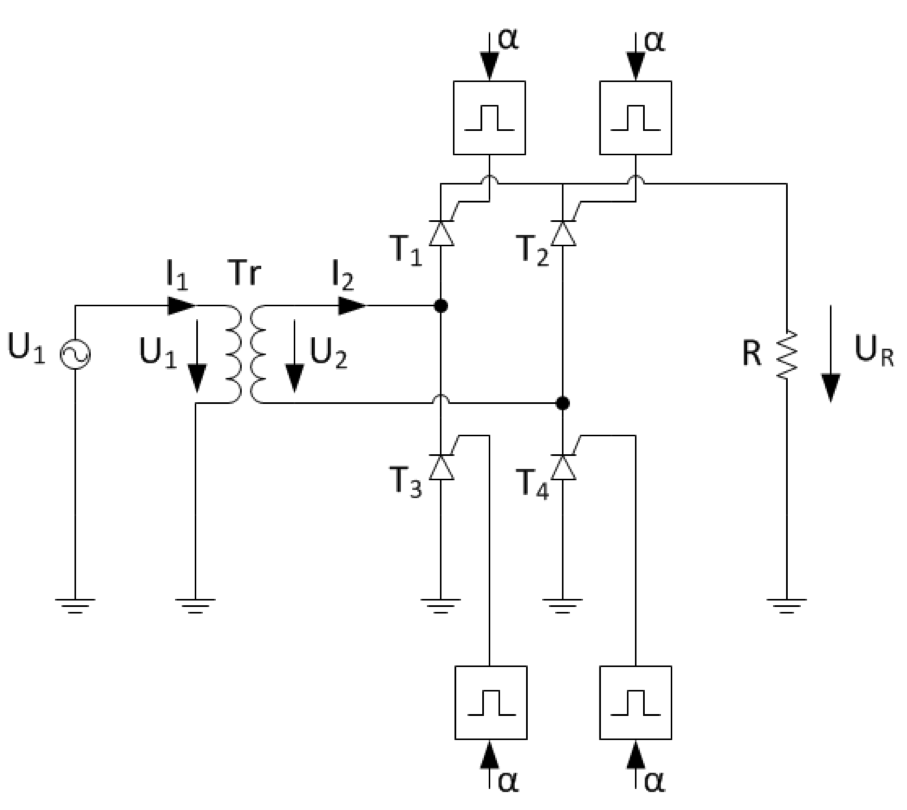
\includegraphics[width=0.85\linewidth]{images/B1C.png}
\end{center}

Der B2C-Gleichrichter verwendet Thyristoren anstelle von Dioden.
Die Gleichspannung ist über den Zündwinkel $\alpha$ steuerbar.

Momentane Ausgangsspannung:
\[
u_d(t) =
\begin{cases}
u_s(t), & \omega t \ge \alpha \\
0, & \omega t < \alpha
\end{cases}
\]

Mittelwert:
\[
\cbl{\overline{u_d} = \frac{2\hat U}{\pi}\cos\alpha}
\]

Eigenschaften:
\begin{itemize}
    \item Stellbereich: $0 \le \alpha \le \pi$
    \item Bei $\alpha > 90^\circ$: Rückspeisebetrieb möglich
    \item Phasenanschnittsteuerung
\end{itemize}

% --- bestehende Grafik: Zündwinkeldiagramm ---
\begin{center}
    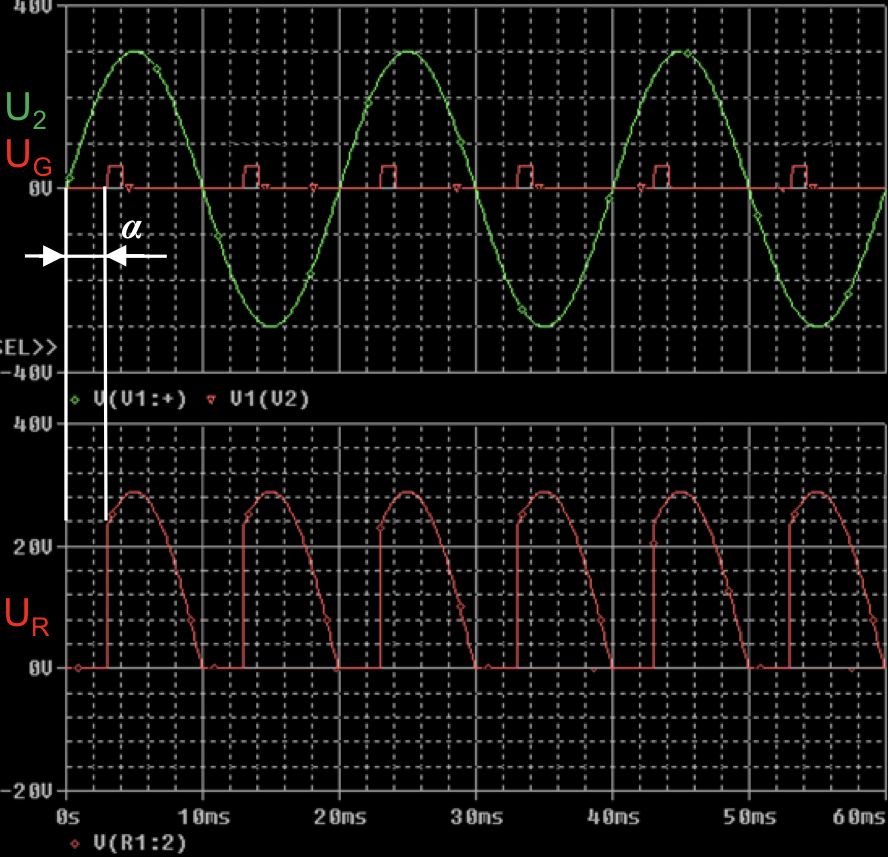
\includegraphics[width=0.85\linewidth]{images/B1C_Verlauf.png}
\end{center}
% -------------------------------------------------

\subsection{Vergleich B2U -- B2C}

\begin{center}
\begin{tabular}{l|c|c}
 & B2U & B2C \\ \hline
Bauelement & Diode & Thyristor \\
Steuerbar & nein & \cbl{ja} \\
Stellgrösse & keine & Zündwinkel $\alpha$ \\
Rückspeisung & nein & möglich \\
\end{tabular}
\end{center}

        \section{Dreiphasiger Gleichrichter}

\subsection{B6U: Ungesteuerter Dreiphasen-Brückengleichrichter}

% --- bestehende Grafik: B6U Schaltung ---
\begin{center}
\centering
    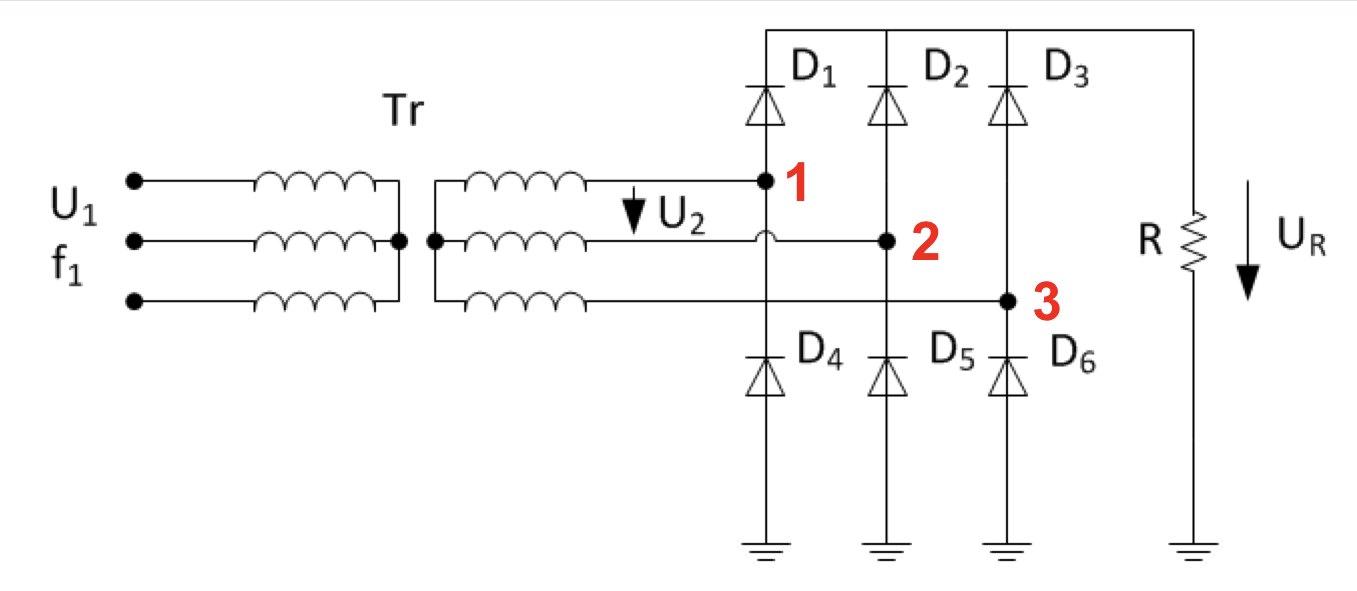
\includegraphics[width=0.65\linewidth]{images/B6U.png}
\end{center}
Zeitverlauf B6U-Gleichrichter:
\begin{center}
    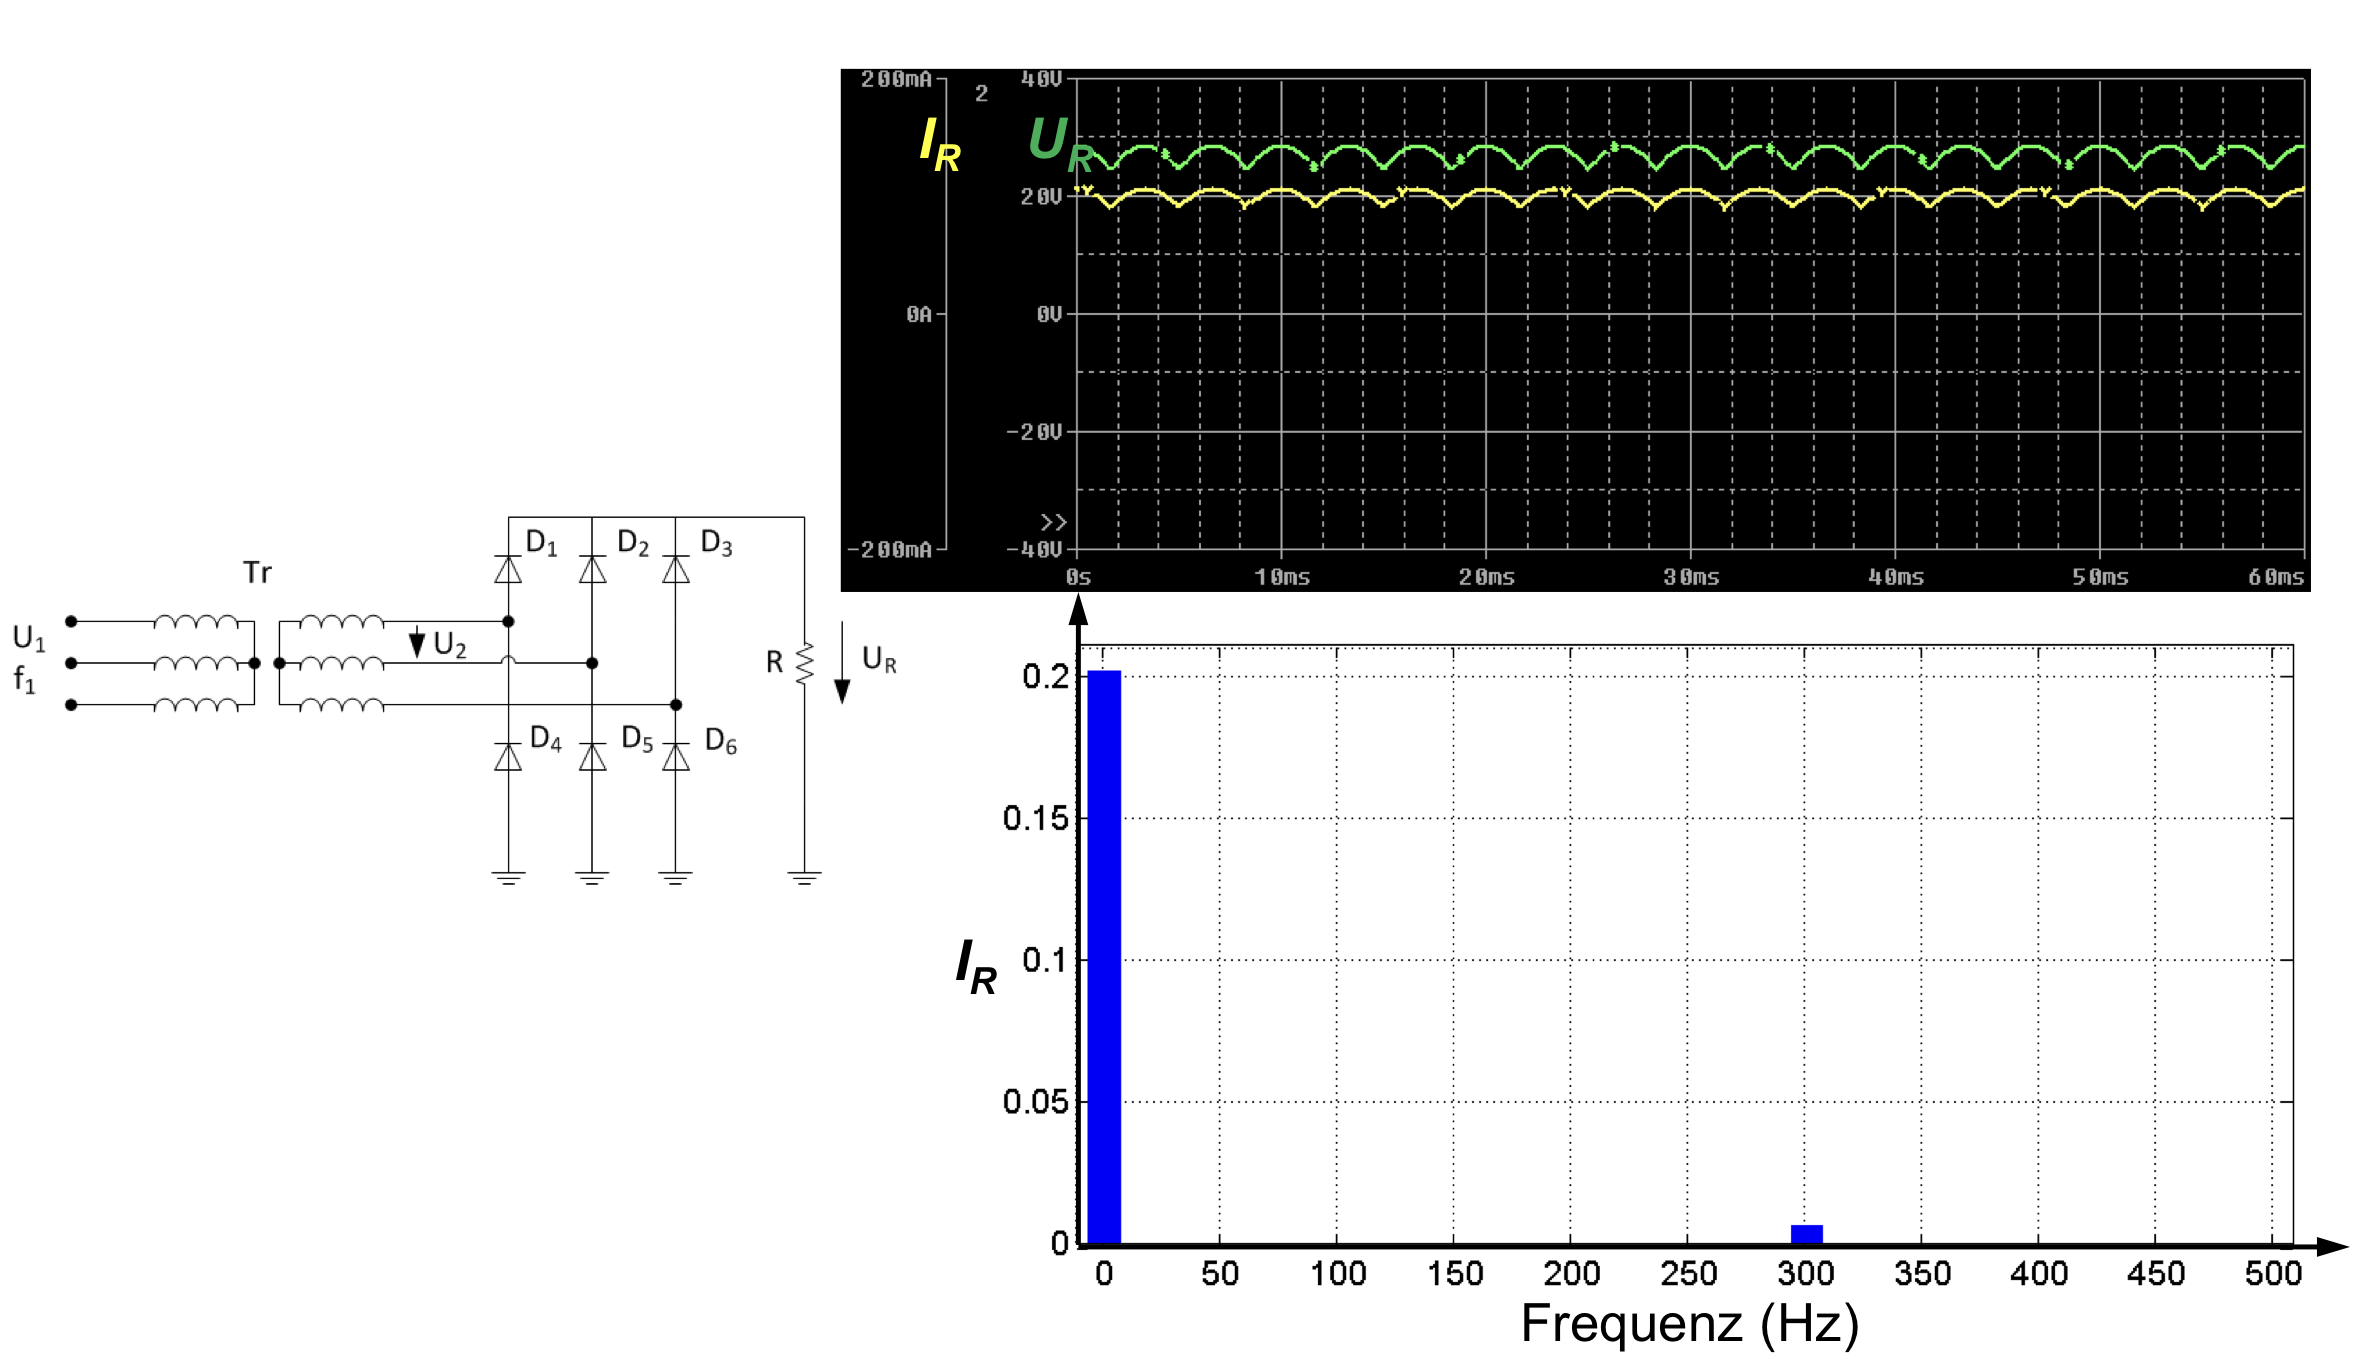
\includegraphics[width=0.85\linewidth]{images/B6U_verlauf.png}
\end{center}
Der B6U-Gleichrichter ist eine dreiphasige Brückenschaltung mit sechs Dioden.
Die Pulszahl beträgt $p=6$.

Mittelwert der Gleichspannung:
\[
\cbl{\overline{u_d} = \frac{3\sqrt{2}}{\pi} U_{LL}}
\]

Eigenschaften:
\begin{itemize}
    \item Sehr geringe Restwelligkeit
    \item Hohe Gleichspannungsqualität
    \item Standard in Industrieanwendungen
\end{itemize}

% -------------------------------------------------

\subsection{B6C: Gesteuerter Dreiphasen-Brückengleichrichter}

% --- bestehende Grafik: B6C Schaltung ---
\begin{center}
    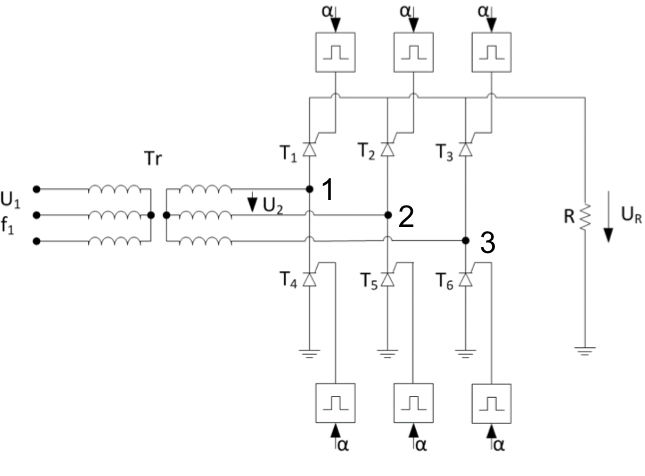
\includegraphics[width=0.65\linewidth]{images/B6C.png}
\end{center}
Zeitverlauf B6C-Gleichrichter:
\begin{center}
    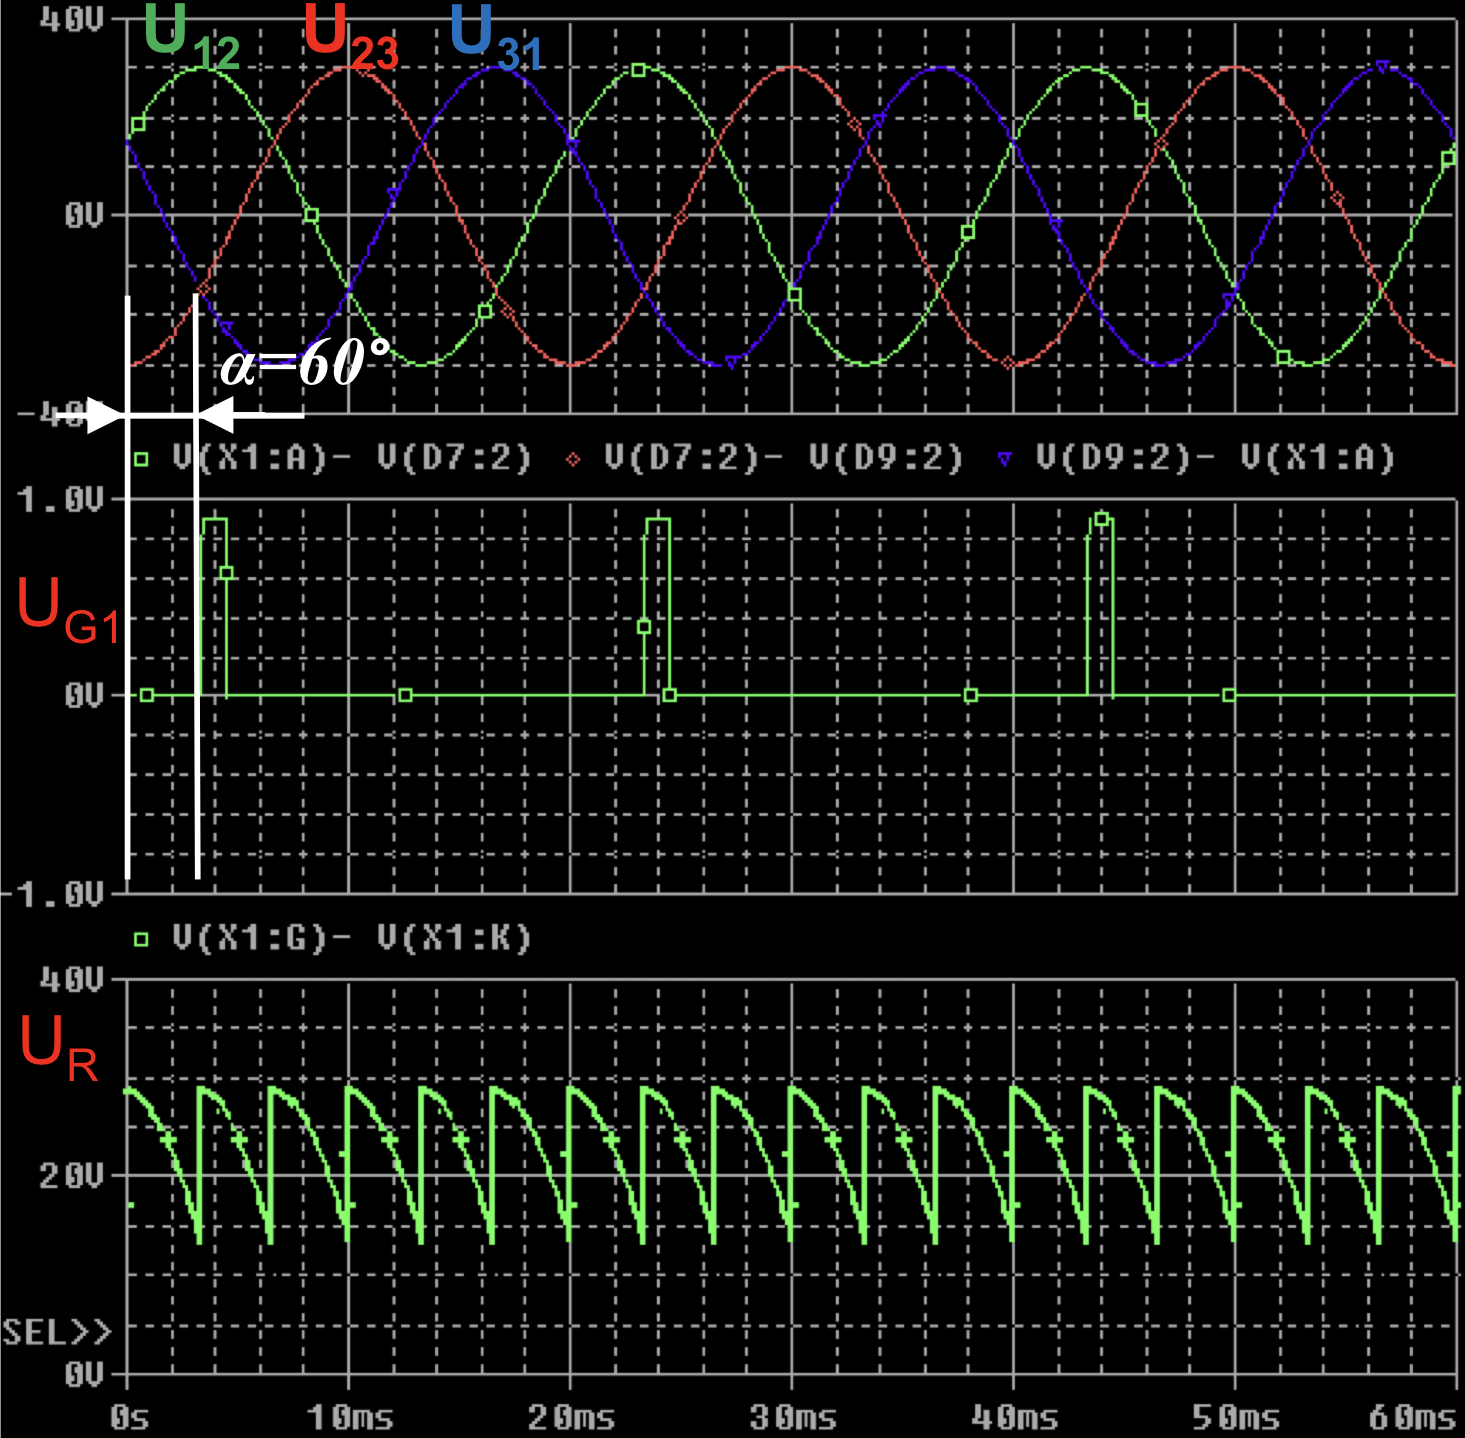
\includegraphics[width=0.85\linewidth]{images/B6C_Verlauf.png}
\end{center}
Beim B6C-Gleichrichter werden die Dioden durch Thyristoren ersetzt.
Die Stellgrösse ist der Zündwinkel $\alpha$.

Mittelwert:
\[
\cbl{\overline{u_d} = \frac{3\sqrt{2}}{\pi} U_{LL} \cos\alpha}
\]

Eigenschaften:
\begin{itemize}
    \item Stellbereich: $0 \le \alpha \le \pi$
    \item Rückspeisebetrieb bei $\alpha > 90^\circ$
    \item Vierquadrantenbetrieb möglich
\end{itemize}

% -------------------------------------------------

\subsection{Kommutierungsüberlappung}

% --- bestehende oder neue Grafik: Überlappung ---
\begin{figure}[h]
\centering
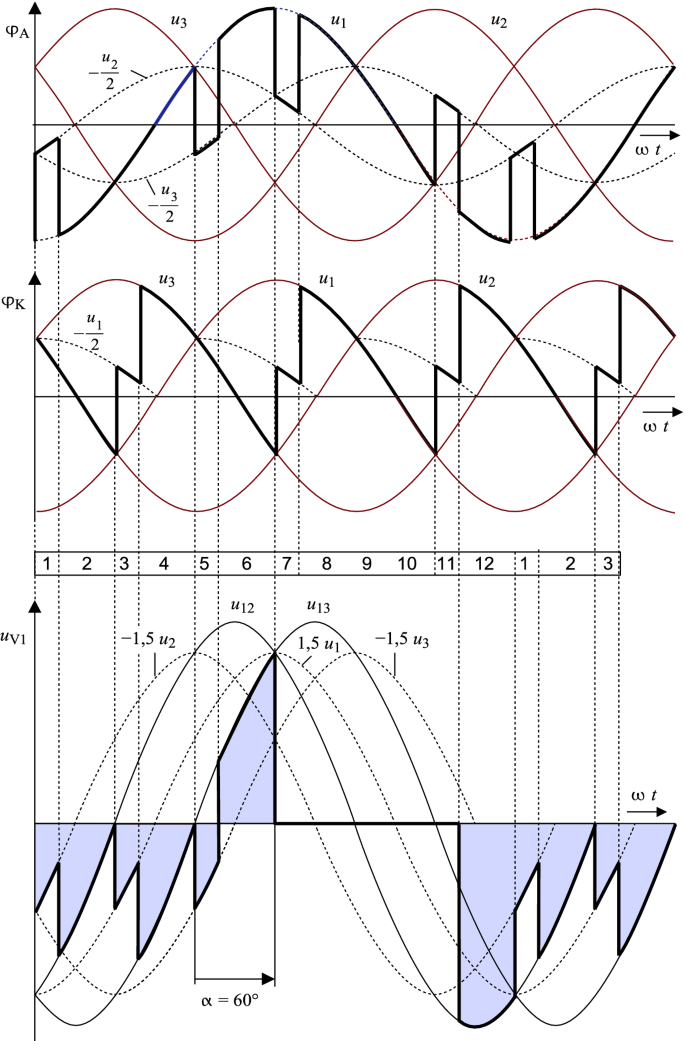
\includegraphics[width=0.65\linewidth]{images/kommutierung.png}
\caption{Kommutierungsüberlappung $\mu$ beim B6-Gleichrichter}
\end{figure}

In realen Netzen ist die Netzinduktivität $L_\sigma$ nicht null.
Dadurch kann der Strom nicht sprunghaft umschalten.
Während der Überlappung leiten \textbf{drei} Ventile gleichzeitig.

Grundgleichung:
\[
\cbl{u_\sigma(t) = L_\sigma \frac{di(t)}{dt}}
\]

Spannungsabfall:
\[
\cbl{\Delta u_d \propto \omega L_\sigma i_d}
\]

Aussage:
\begin{itemize}
    \item $L_\sigma \uparrow \Rightarrow \overline{u_d} \downarrow$
    \item $i_d \uparrow \Rightarrow \overline{u_d} \downarrow$
\end{itemize}

\paragraph{Überlappungsverlust bei Netzinduktivität}
Bei endlicher Netzinduktivität $L_\sigma$ ergibt sich ein zusätzlicher Spannungsabfall:
\[
\Delta u_d = \frac{3}{\pi} \, \omega L_\sigma i_d
\]
Damit:
\[
u_d = \frac{3\sqrt{2}}{\pi} U_{LL} \cos\alpha - \Delta u_d
\]


% -------------------------------------------------

\subsection{Netzströme und Harmonische}

% --- bestehende Grafik: Netzstrom ---
\begin{figure}[h]
\centering
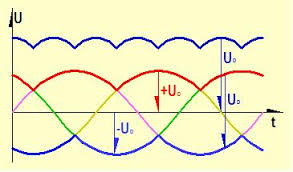
\includegraphics[width=0.7\linewidth]{images/B6strom.png}
\caption{Leiterstrom beim B6-Gleichrichter}
\end{figure}

Bei grosser Glättinduktivität ist der Gleichstrom $i_d$ näherungsweise konstant.
Die Leiterströme sind rechteckförmig (120$^\circ$-Leitung).

Harmonische Ordnung:
\[
\cbl{n = 6k \pm 1 \qquad (k \in \mathbb{N})}
\]

Dominant:
\[
\cbl{5,\;7,\;11,\;13,\;\dots}
\]

Nicht vorhanden:
\[
\cbl{3,\;9,\;15,\;\dots}
\]

% -------------------------------------------------

\subsection{Vergleich B2 -- B6}

\begin{center}
\begin{tabular}{l|c|c}
 & B2 & B6 \\ \hline
Pulszahl & 2 & \cbl{6} \\
Restwelligkeit & hoch & \cbl{gering} \\
Gleichspannungsqualität & gering & \cbl{hoch} \\
Netzstrom & stärker verzerrt & \cbl{weniger verzerrt} \\
\end{tabular}
\end{center}

\subsection{Merksätze}

\begin{itemize}
    \item B6 ist der wichtigste industrielle Gleichrichter.
    \item Mittelwert proportional zu $\cos\alpha$ beim B6C.
    \item Netzstromharmonische: $6k \pm 1$.
\end{itemize}

        \section{Wechselstromschalter und Wechselstromsteller}

\subsection{Wechselstromschalter}

% --- bestehende Grafik: AC-Schalter ---
Wechselstromschalter mit bidirektionalem Ventil
\begin{center}
    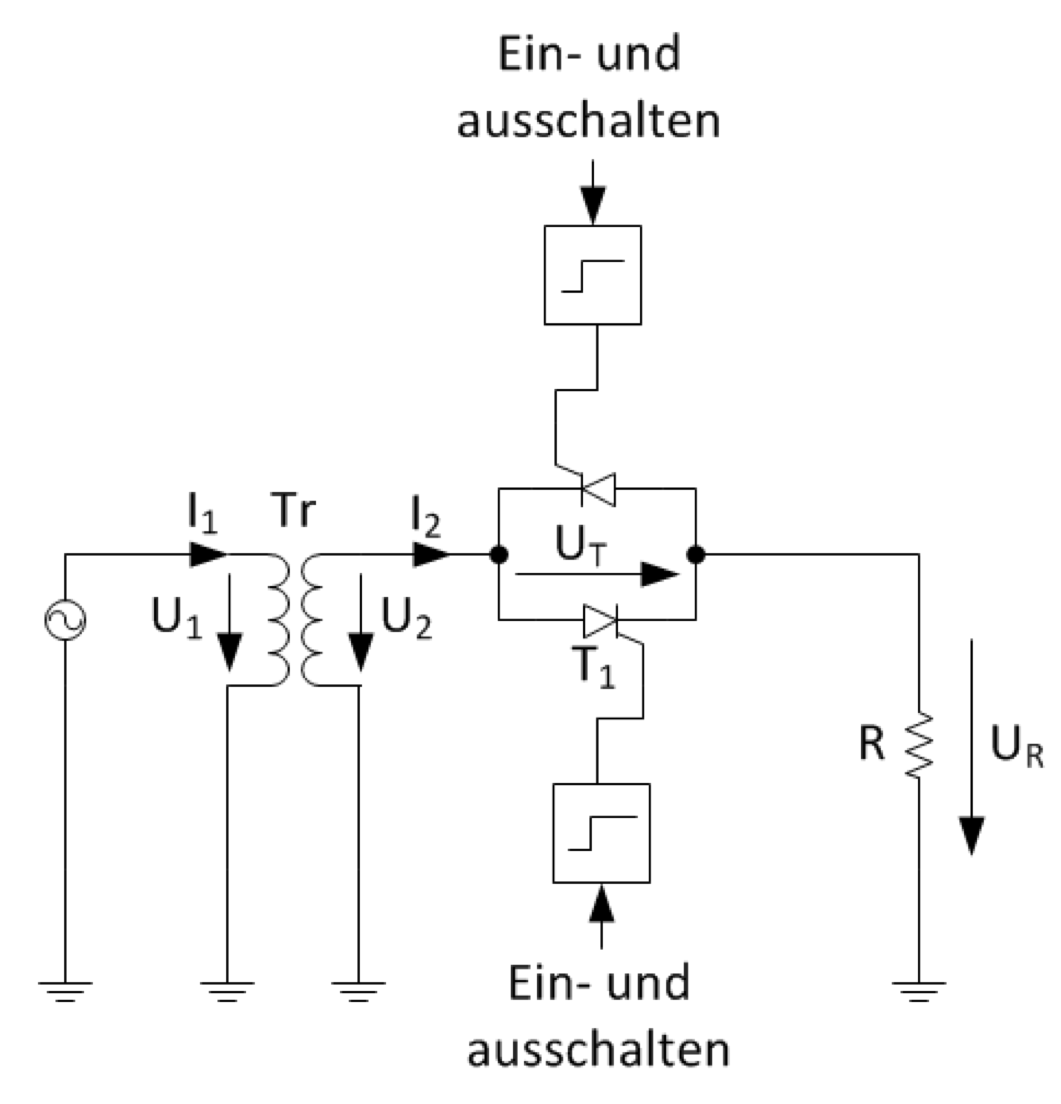
\includegraphics[width=0.85\linewidth]{images/Wechselstromschalter.png}
\end{center}
Ein Wechselstromschalter dient zum reinen \textbf{Ein- und Ausschalten} einer Wechselspannung.
Es findet \textbf{keine Stellfunktion} statt.

Eigenschaften:
\begin{itemize}
    \item Steuerung: Ein/Aus
    \item Keine Spannungsformänderung
    \item Typische Bauelemente: Relais, Triac, antiparallele Thyristoren
\end{itemize}

\crd{\textrightarrow\ Wechselstromschalter sind keine Steller.}

% -------------------------------------------------

\subsection{Wechselstromsteller (Phasenanschnittsteller)}

% --- bestehende Grafik: Phasenanschnitt ---
Phasenanschnittsteuerung beim Wechselstromsteller
\begin{center}
    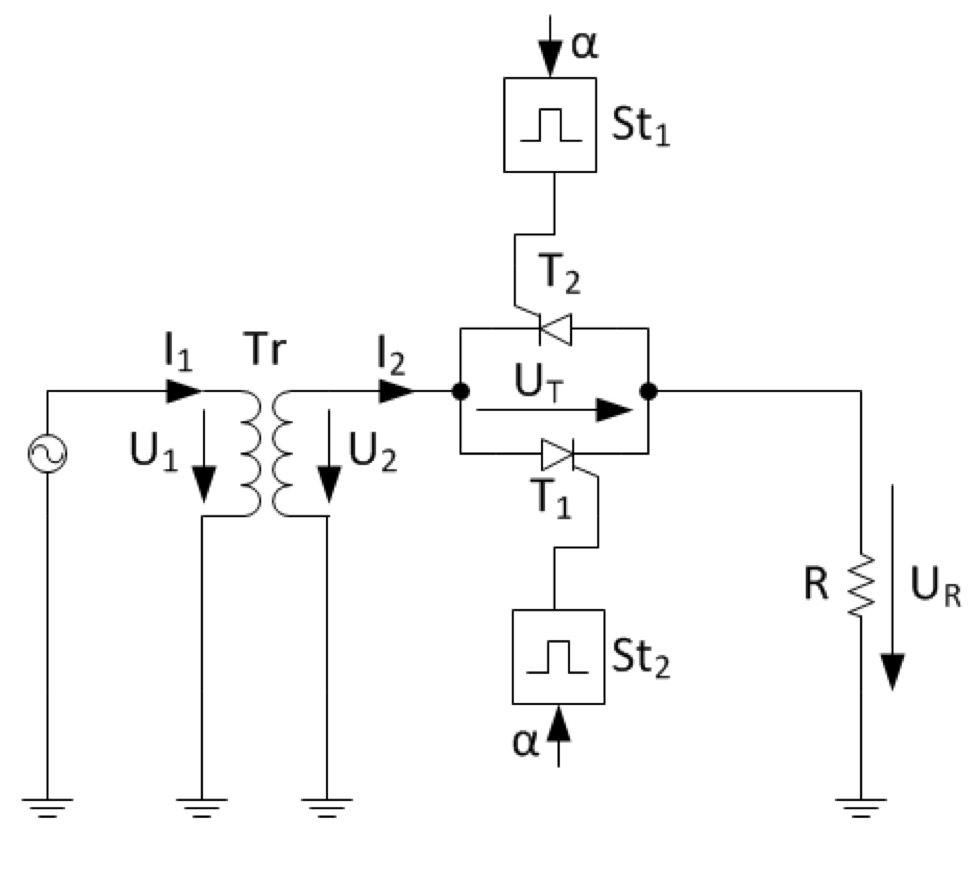
\includegraphics[width=0.85\linewidth]{images/Wechselstromsteller.png}
\end{center}

Ein Wechselstromsteller wandelt eine konstante Wechselspannung in eine \textbf{veränderliche Wechselspannung}.
Die Stellgrösse ist der Zündwinkel $\alpha$.

Momentane Ausgangsspannung:
\[
u(t) =
\begin{cases}
u_s(t), & \omega t \ge \alpha \\
0, & \omega t < \alpha
\end{cases}
\]

Effektivwert (R-Last):
\[
\cbl{U_{\mathrm{RMS}}(\alpha) = U \sqrt{\frac{1}{\pi} \int_\alpha^\pi \sin^2\theta \, d\theta}}
\]

\paragraph{Geschlossene Formel für Effektivwert (R-Last)}
\[
U_{\mathrm{RMS}}(\alpha) = U_s \sqrt{\frac{1}{2\pi} \left( \pi - \alpha + \frac{1}{2}\sin 2\alpha \right)}
\]

Eigenschaften:
\begin{itemize}
    \item Stellgrösse: Zündwinkel $\alpha$
    \item Nichtsinusförmige Spannung
    \item Einsatz: Heizung, Lichtdimmer
\end{itemize}

\subsection{Abgrenzung Schalter -- Steller}

\begin{center}
\begin{tabular}{l|c|c}
 & Schalter & Steller \\ \hline
Funktion & Ein/Aus & \cbl{Stellbar} \\
Stellgrösse & keine & Zündwinkel $\alpha$ \\
Spannungsform & unverändert & \cbl{verformt} \\
\end{tabular}
\end{center}

        \section{Gleichstromsteller (Chopper)}

Ein Gleichstromsteller wandelt eine konstante Gleichspannung $U_{DC}$ in eine
\textbf{stufenlos einstellbare Gleichspannung} $u_d$ durch schnelles Ein- und Ausschalten
eines Halbleiterschalters.

Typische Anwendungen:
\begin{itemize}
\item Drehzahlregelung von Gleichstrommaschinen,
\item Stromregelung in Antrieben,
\item DC-Zwischenkreise in Umrichtern.
\end{itemize}

Die Stellgrösse ist der \textbf{Tastgrad}:
\[
\boxed{d = \frac{t_{\mathrm{on}}}{T_s}}, 
\qquad T_s = \text{Schaltperiode}
\]

\subsection{Grundprinzip}

% --- bestehende Grafik: Grundschaltung Chopper ---
\begin{center}
    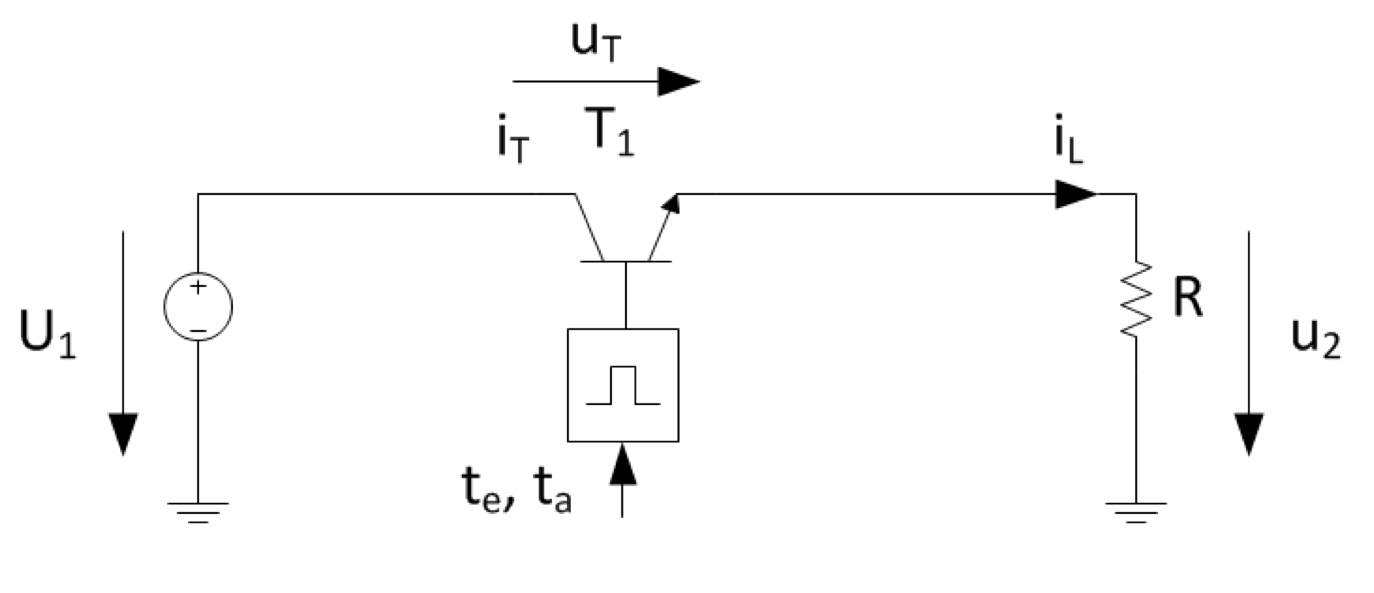
\includegraphics[width=0.85\linewidth]{images/Gleichstromsteller.png}
\end{center}

Während der Einschaltzeit $t_{\mathrm{on}}$ gilt:
\[
u_d(t) = U_{DC}
\]

Während der Ausschaltzeit $t_{\mathrm{off}}$ gilt (idealer Freilauf):
\[
u_d(t) = 0
\]

Mittelwert der Ausgangsspannung:
\[
\boxed{u_d = d \, U_{DC}}
\]

Dies ist identisch zum \textbf{Buck-Wandler} im kontinuierlichen Betrieb.

\subsection{Zeitbereich bei R--L-Last}

Bei R--L-Last gilt stückweise:

\paragraph{EIN-Phase}

\[
L \frac{di}{dt} + R i = U_{DC}
\]

Lösung:
\[
\boxed{
i(t) = \frac{U_{DC}}{R} + \left(i_{\min} - \frac{U_{DC}}{R}\right) e^{-t/\tau}
}, 
\qquad \tau = \frac{L}{R}
\]

\paragraph{AUS-Phase}

\[
L \frac{di}{dt} + R i = 0
\]

\[
\boxed{
i(t) = i_{\max} \, e^{-t/\tau}
}
\]

Periodenbedingung:
\[
\boxed{i_{\min} = i_{\max} \, e^{-T_a/\tau}}
\]

\subsection{Stromrippel und kontinuierlicher Betrieb}

Stromrippel:
\[
\boxed{
\Delta i = i_{\max} - i_{\min}
}
\]

Näherung für kleines R:
\[
\boxed{
\Delta i \approx \frac{(U_{DC} - u_d)\, d T_s}{L}
}
\]

Grenzinduktivität für kontinuierlichen Betrieb:
\[
\boxed{
L_{\min} = \frac{(1-d)R}{2 f_s}
}
\]

\begin{itemize}
\item $L > L_{\min}$ $\Rightarrow$ kontinuierlicher Betrieb (CCM),
\item $L < L_{\min}$ $\Rightarrow$ diskontinuierlicher Betrieb (DCM),
\item DCM $\Rightarrow$ Mittelwertformel $u_d = dU_{DC}$ gilt nicht mehr exakt.
\end{itemize}

\subsection{Einquadrantensteller (1Q)}

% --- bestehende Grafik: 1Q ---
\begin{center}
    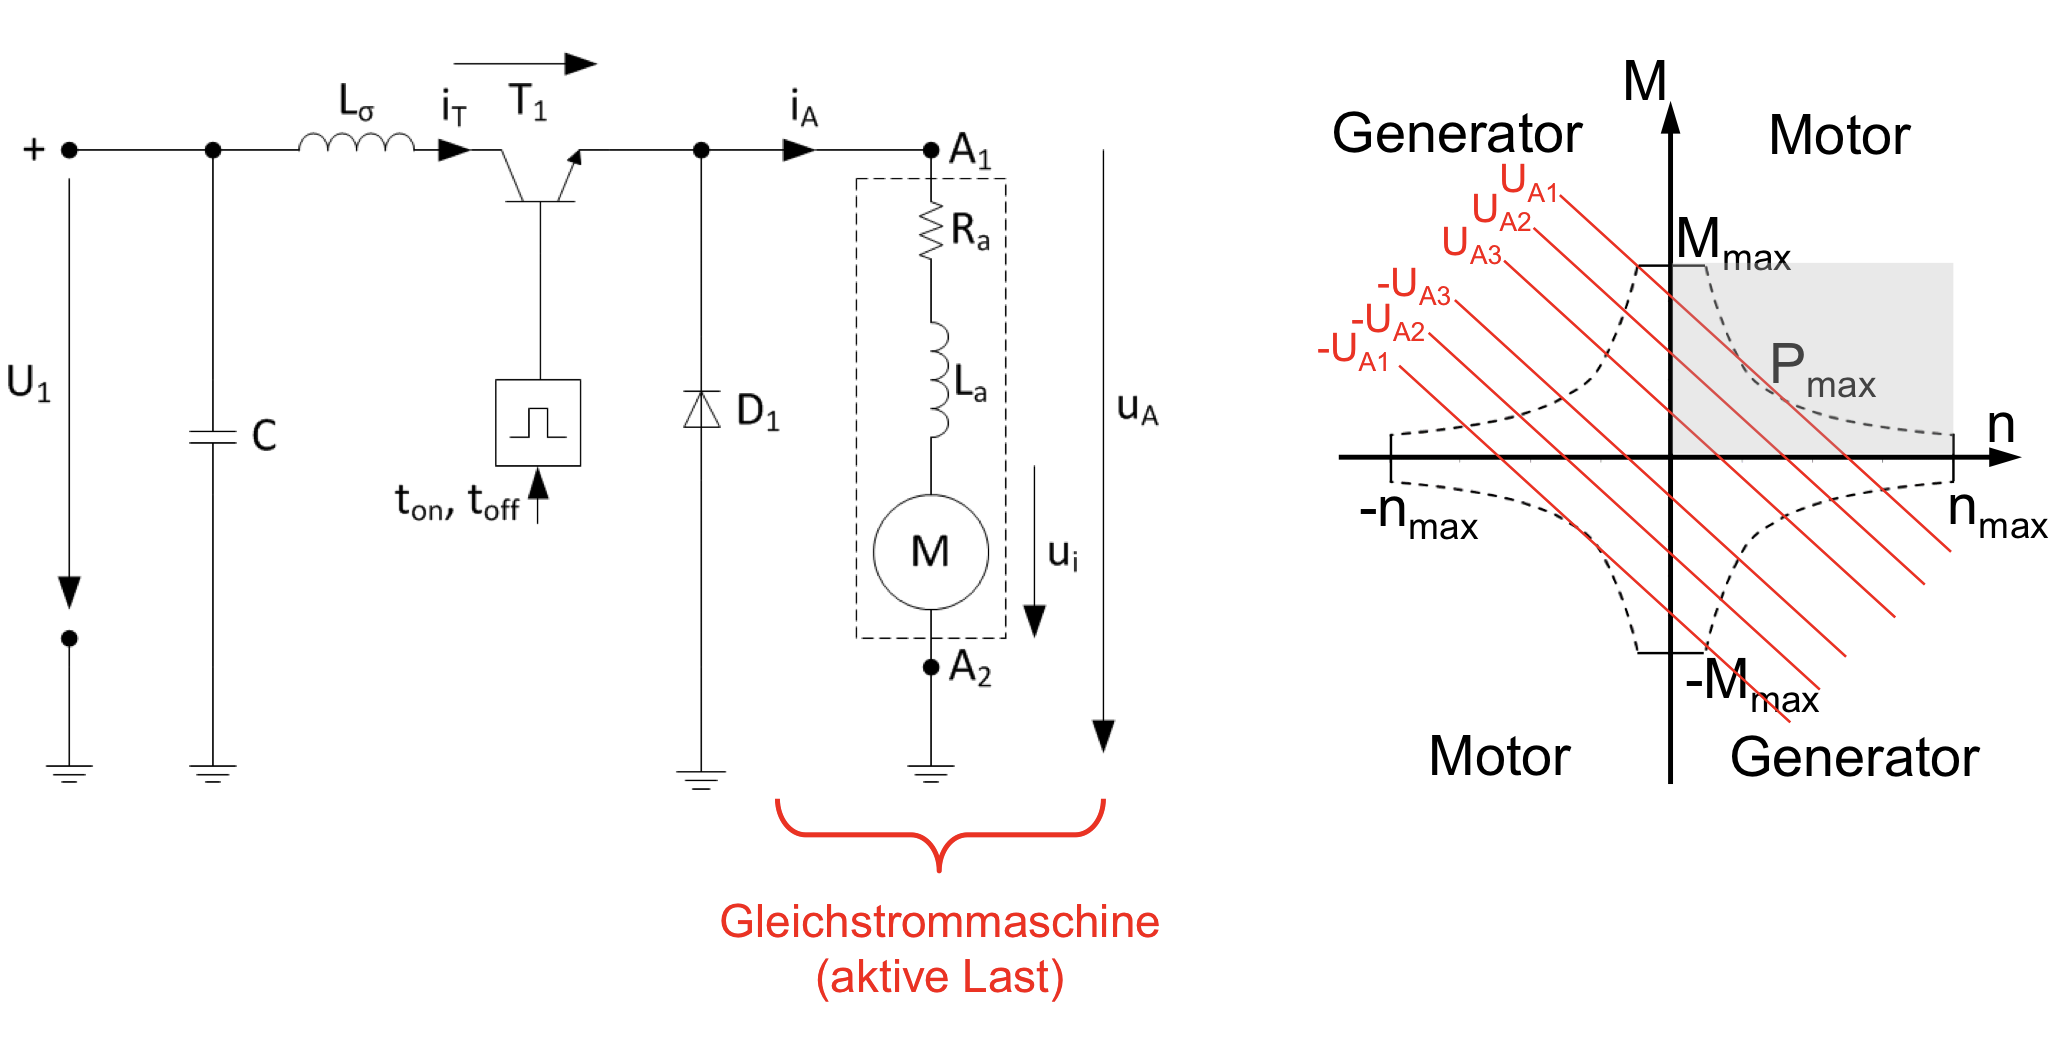
\includegraphics[width=0.85\linewidth]{images/Gleichstromsteller1Q.png}
\end{center}

Eigenschaften:
\begin{itemize}
\item $u_d \ge 0$, $i_d \ge 0$
\item Nur \textbf{Motorbetrieb vorwärts}
\end{itemize}

Spannungssteuerung:
\[
\boxed{u_d = d \, U_{DC}}
\]

Leistungsfluss:
\[
\boxed{P = u_d \, i_d > 0}
\]

Einsatz:
\begin{itemize}
\item Einfache Drehzahlregelung von Gleichstrommotoren,
\item Stromquellenbetrieb.
\end{itemize}

\subsection{Zweiquadrantensteller (2Q)}

% --- bestehende Grafik: 2Q ---
\begin{center}
    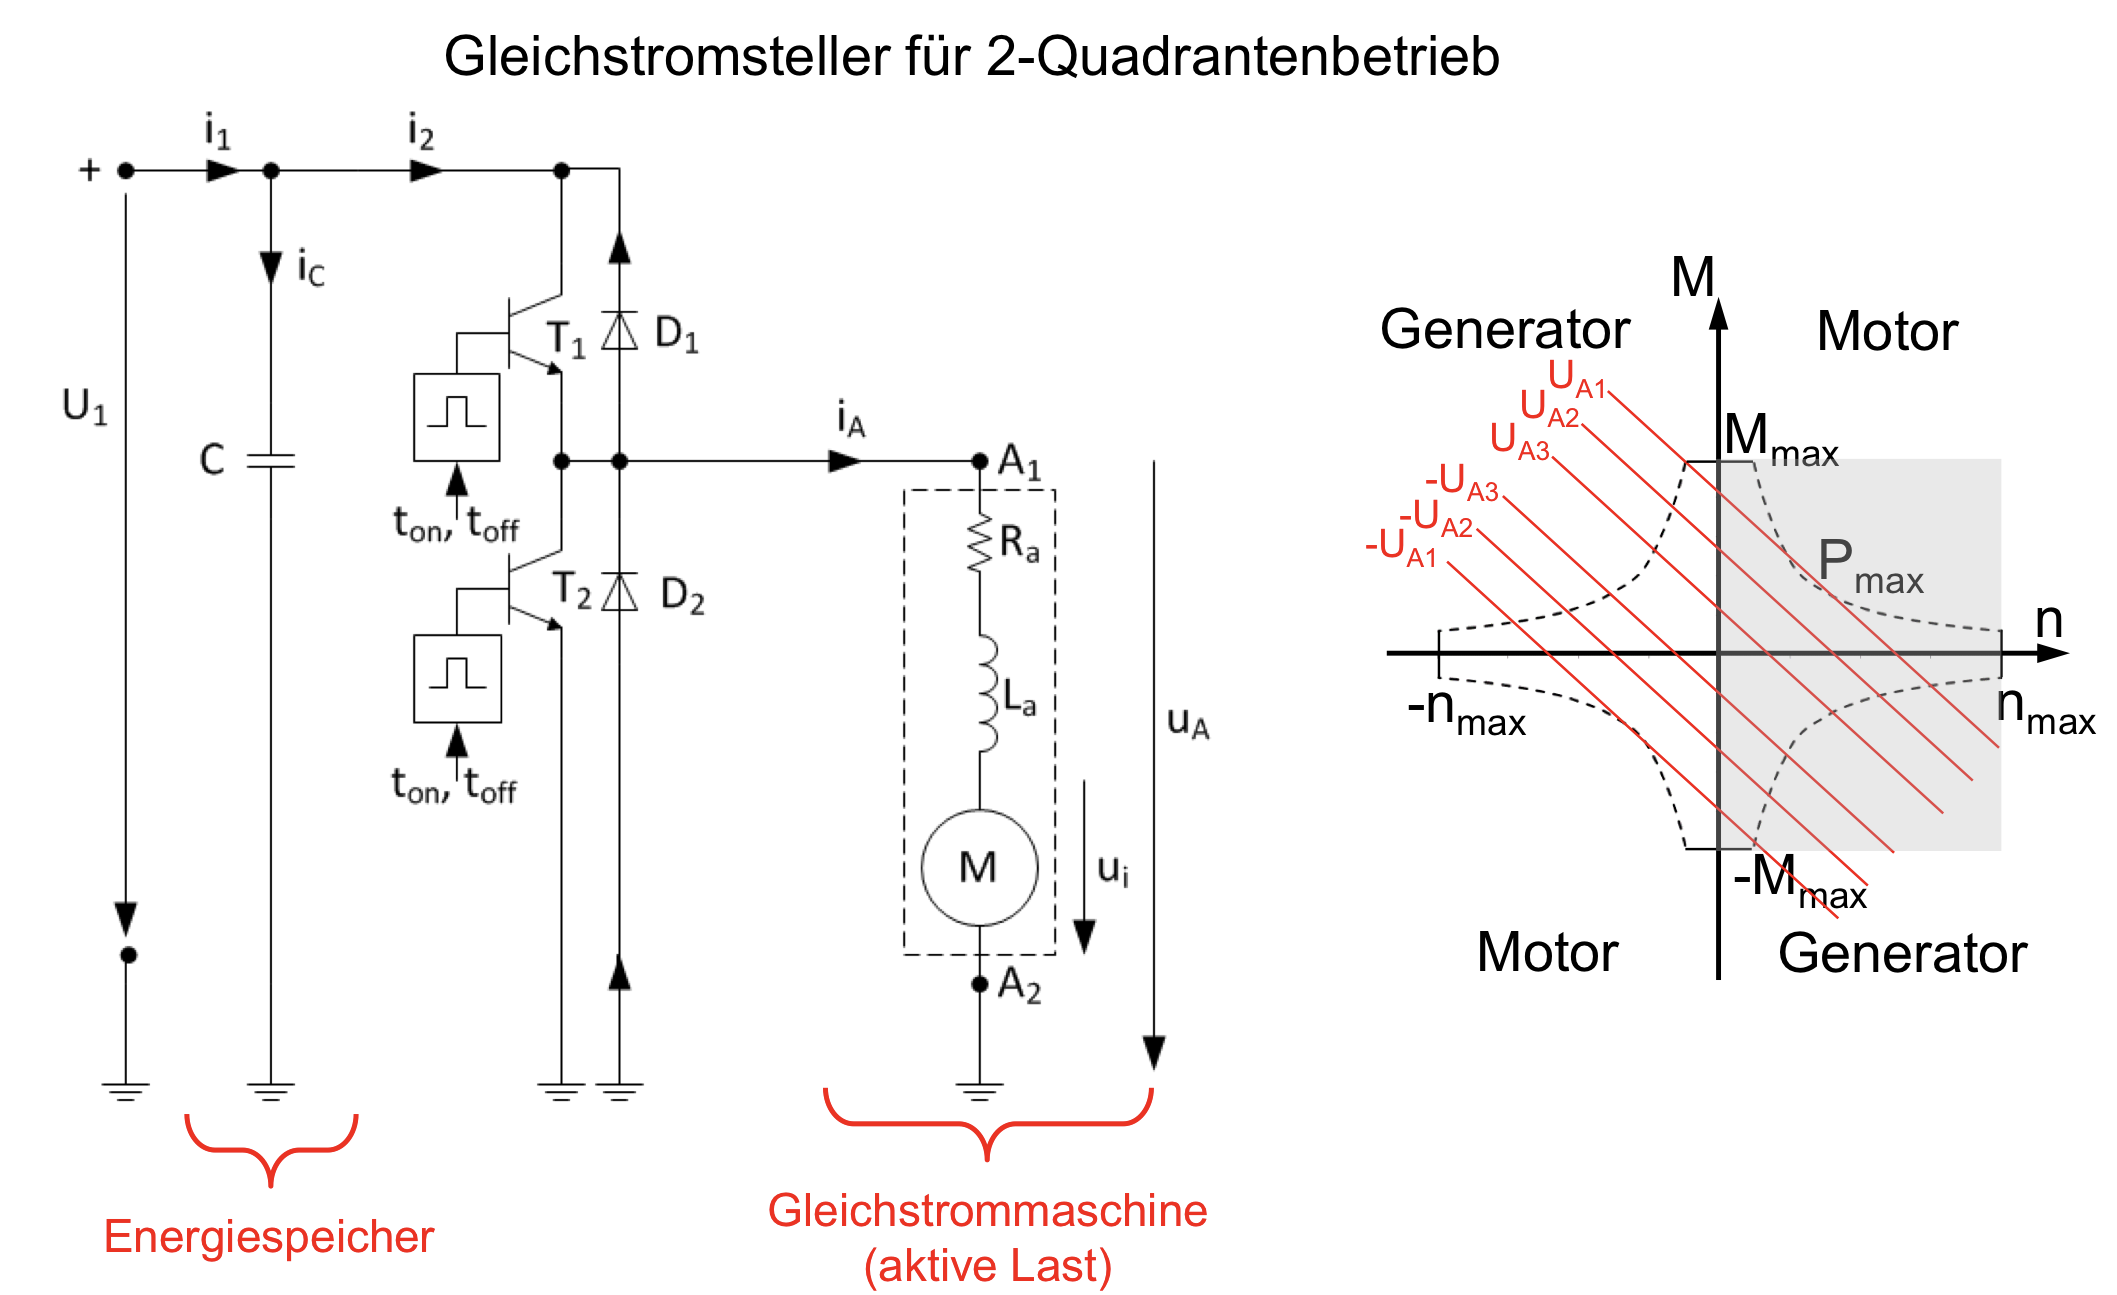
\includegraphics[width=0.85\linewidth]{images/Gleichstromsteller2Q.png}
\end{center}

Eigenschaften:
\begin{itemize}
\item $u_d \ge 0$
\item $i_d$ kann Vorzeichen wechseln
\item Motorbetrieb und \textbf{generatorischer Bremsbetrieb}
\end{itemize}

Beim Rekuperieren:
\[
\boxed{P = u_d \, i_d < 0}
\]

\begin{itemize}
\item Energie fliesst vom Motor zurück in die Quelle.
\item Typisch für elektrische Bremsung.
\end{itemize}

\subsection{Vierquadrantensteller (4Q)}

% --- bestehende Grafik: 4Q ---
\begin{center}
    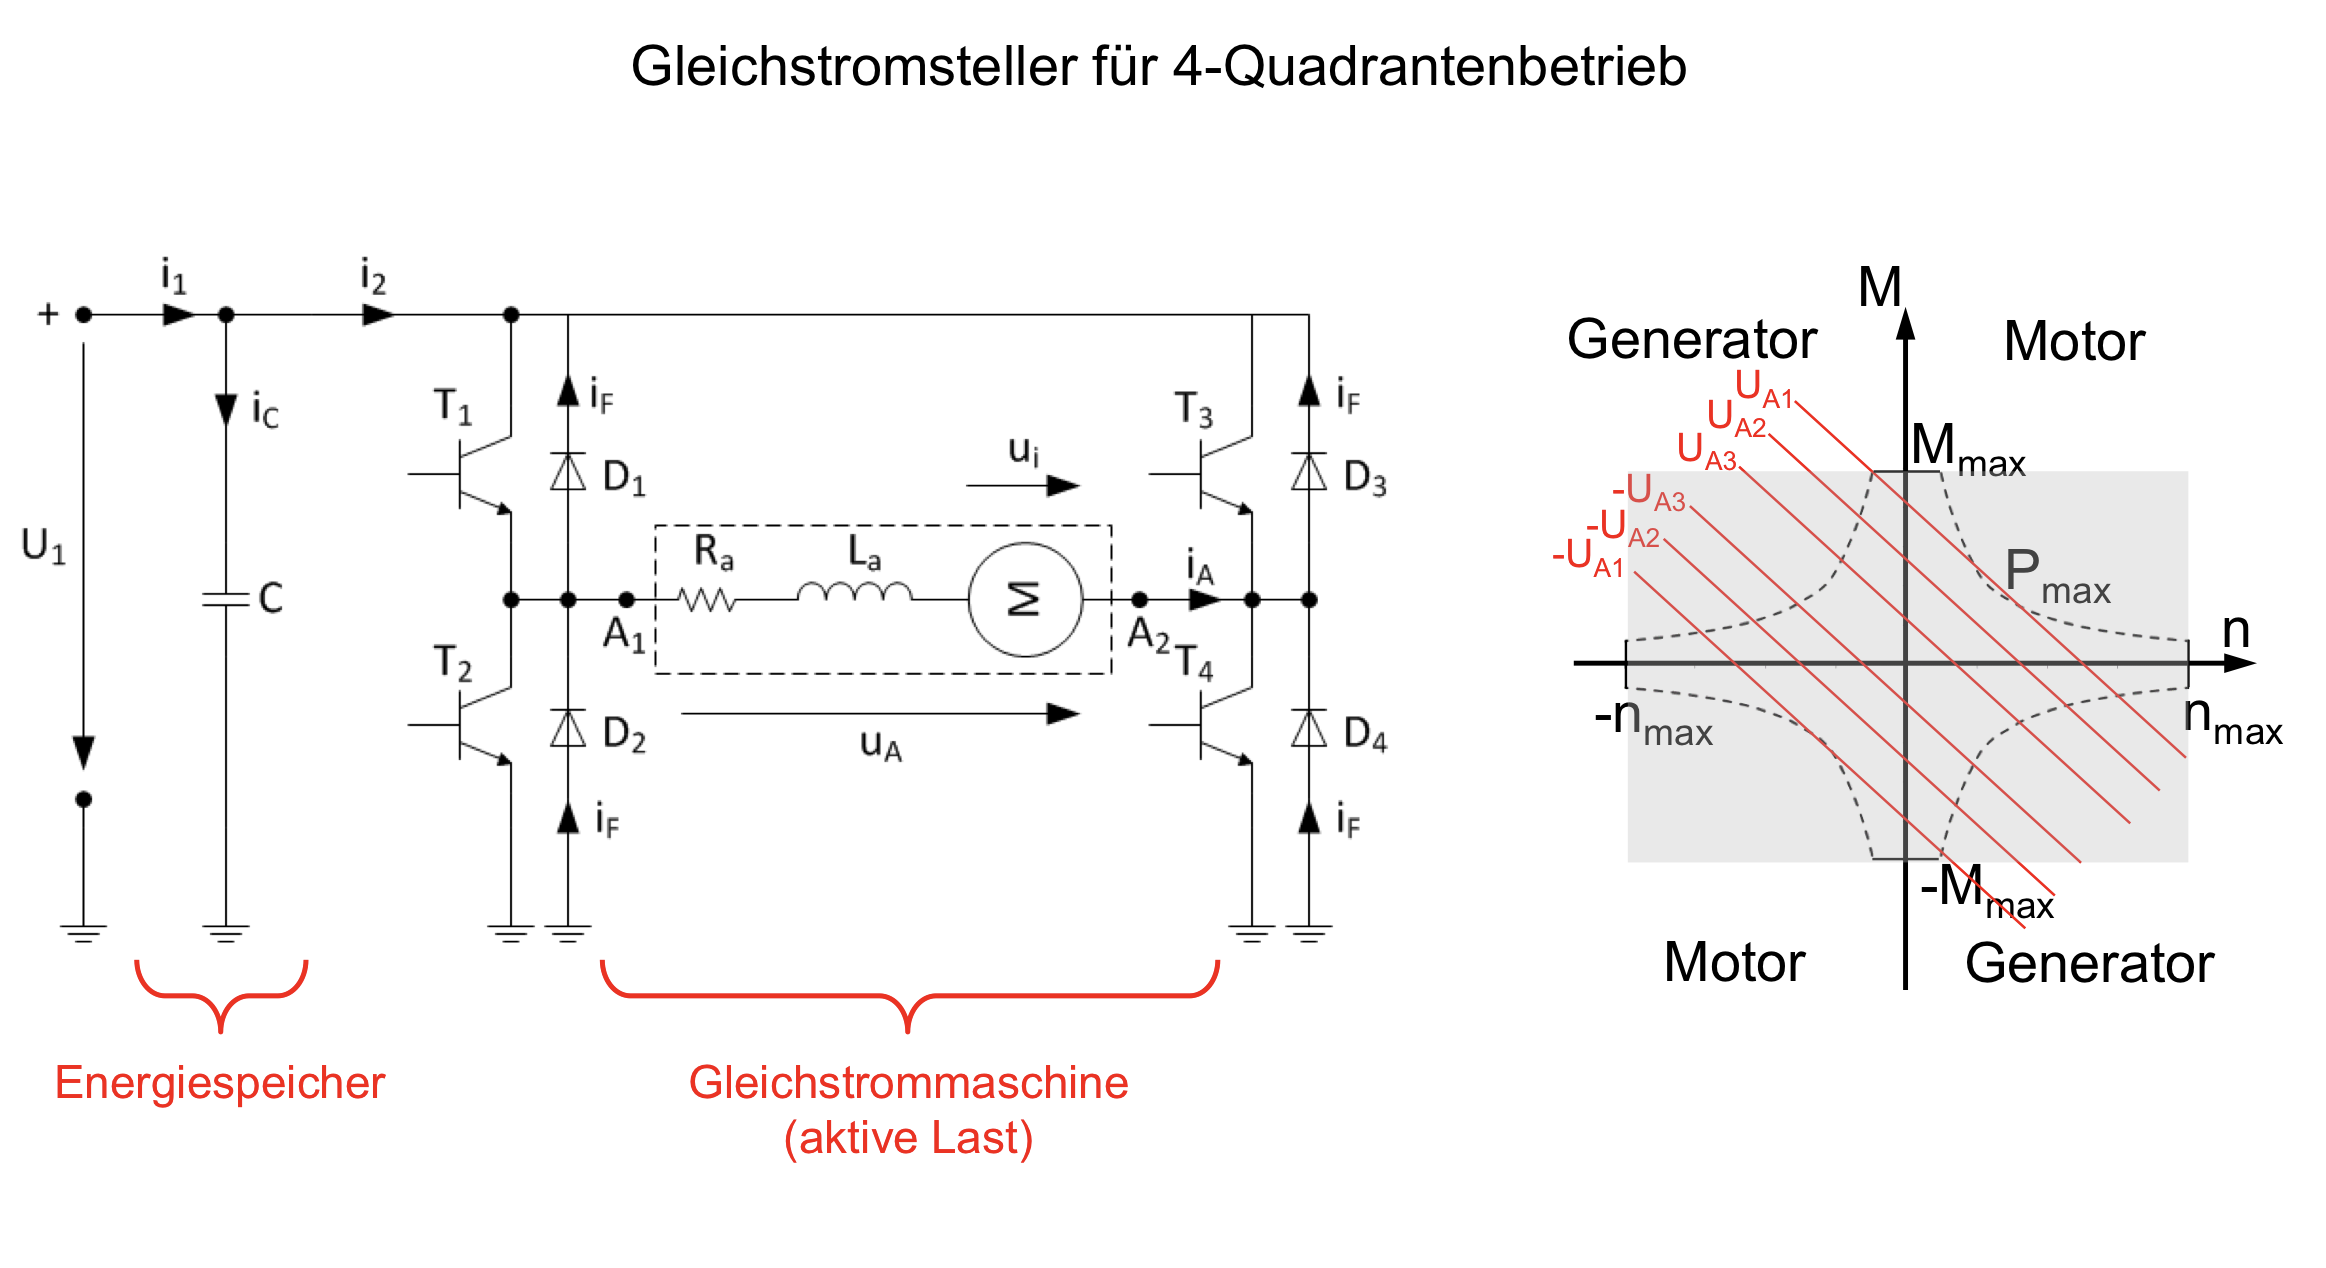
\includegraphics[width=0.85\linewidth]{images/Gleichstromsteller4Q.png}
\end{center}

Eigenschaften:
\begin{itemize}
\item $u_d$ vorzeichenwechselnd,
\item $i_d$ vorzeichenwechselnd,
\item Vollständiger Betrieb in allen Quadranten.
\end{itemize}

Quadranten:
\begin{itemize}
\item I: Motor vorwärts ($u>0,i>0$)
\item II: Generator vorwärts ($u<0,i>0$)
\item III: Motor rückwärts ($u<0,i<0$)
\item IV: Generator rückwärts ($u>0,i<0$)
\end{itemize}

Einsatz:
\begin{itemize}
\item Reversierantriebe,
\item Positionierantriebe,
\item Prüfstände.
\end{itemize}

\subsection{Bezug zur Gleichstrommaschine}

Für die DC-Maschine gilt:
\[
\boxed{u_d = R_a i_a + k\Phi \omega}
\]

Daraus:
\[
\boxed{\omega \approx \frac{u_d}{k\Phi} \quad \text{(bei kleiner Last)}}
\]

\begin{itemize}
\item $d\uparrow \Rightarrow u_d\uparrow \Rightarrow \omega\uparrow$
\item $d\downarrow \Rightarrow u_d\downarrow \Rightarrow \omega\downarrow$
\item Gleichstromsteller ist das \textbf{Standard-Stellglied} für DC-Antriebe.
\end{itemize}

\subsection{Vergleich zu Gleichrichtern}

\begin{itemize}
\item Gleichrichter: Spannung über Zündwinkel $\alpha$ gesteuert.
\item Gleichstromsteller: Spannung über Tastgrad $d$ gesteuert.
\item Gleichstromsteller arbeitet mit \textbf{hoher Schaltfrequenz}.
\item Gleichrichter arbeitet mit \textbf{Netzfrequenz}.
\end{itemize}

\subsection{Merksätze}

\begin{itemize}
\item Stellgrösse beim Gleichstromsteller ist der \textbf{Tastgrad $d$}.
\item $u_d = d U_{DC}$ gilt nur im \textbf{kontinuierlichen Betrieb}.
\item 1Q: nur Motorbetrieb vorwärts.
\item 2Q: Motor + generatorisches Bremsen.
\item 4Q: Motor und Generator in beiden Drehrichtungen.
\item Gleichstromsteller = Buck-Wandler für Antriebe.
\end{itemize}

        \section{Gleichstrommaschine im Umrichterbetrieb}

Diese Section behandelt die \textbf{Gleichstrommaschine} als Last und Antrieb
im Zusammenspiel mit Gleichrichtern und Gleichstromstellern.
Sie ist zentral für die Analyse von \textbf{Drehzahl}, \textbf{Drehmoment}, \textbf{Stabilität}
und für das Verständnis der \textbf{Kennlinien $M$–$n$}.

\smallskip

\textbf{Zielbild:}
\begin{itemize}
    \item Grundgleichungen der Gleichstrommaschine kennen
    \item Zusammenhang zwischen Spannung, Strom, Drehzahl und Drehmoment verstehen
    \item Einfluss der Ankerspannung auf die Drehzahl analysieren
    \item Stabilen und instabilen Betrieb beurteilen
\end{itemize}

\subsection{Grundaufbau und Ersatzschaltbild}
\begin{center}
    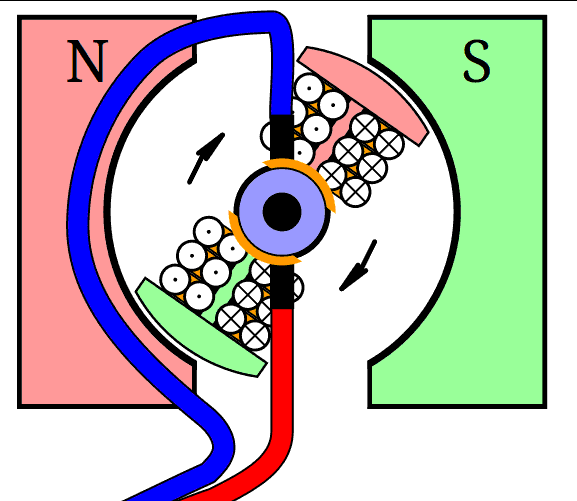
\includegraphics[width=0.85\linewidth]{images/Grundaufbau_gleistrommaschiene.png}
\end{center}
\subsubsection{Vereinfachtes Ersatzschaltbild}

\begin{center}
    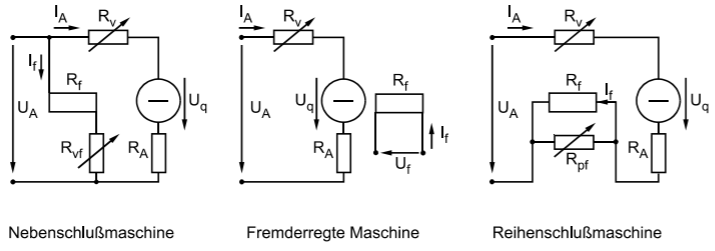
\includegraphics[width=0.85\linewidth]{images/gleichstrommasciene.png}
\end{center}

\textbf{Elemente:}
\begin{itemize}
    \item $u_a(t)$: Ankerspannung aus Umrichter oder Steller
    \item $R_a$: Ankerwiderstand
    \item $L_a$: Ankerinduktivität
    \item $E_i$: induzierte Gegenspannung
    \item $i_a(t)$: Ankerstrom
\end{itemize}

\subsection{Grundgleichungen der Gleichstrommaschine}

\subsubsection{Elektrische Gleichung}

\[
\cbl{u_a(t) = R_a\, i_a(t) + L_a\, \frac{di_a(t)}{dt} + E_i(t).}
\]

\subsubsection{Gegenspannung}

Die induzierte Gegenspannung ist proportional zur Drehzahl:
\[
\cbl{E_i = k_e \, \omega = \omega \, \Psi.}
\]

Dabei:
\begin{itemize}
    \item $\omega$: mechanische Winkelgeschwindigkeit
    \item $\Psi$: Erregerfluss
\end{itemize}

\subsubsection{Drehmomentgleichung}

Das elektromagnetische Drehmoment ist proportional zum Ankerstrom:
\[
\cbl{M = k_m \, i_a = i_a \, \Psi.}
\]

\crd{\textrightarrow\ Drehmoment wird \textbf{direkt durch den Strom} bestimmt.}

\subsection{Mechanische Gleichung}

Die mechanische Bewegungsgleichung lautet:
\[
\cbl{J \frac{d\omega}{dt} = M - M_L - B\,\omega.}
\]

Dabei:
\begin{itemize}
    \item $J$: Trägheitsmoment
    \item $M_L$: Lastmoment
    \item $B$: Reibungskoeffizient
\end{itemize}

Im stationären Betrieb gilt:
\[
M = M_L.
\]

\subsection{Stationärer Betrieb}

Im stationären Gleichgewicht:
\[
\frac{di_a}{dt} = 0, \qquad \frac{d\omega}{dt} = 0.
\]

Damit:
\[
\cbl{u_a = R_a\, i_a + E_i = R_a\, i_a + \omega \Psi.}
\]

Auflösen nach der Drehzahl:
\[
\cbl{\omega = \frac{u_a - R_a i_a}{\Psi}.}
\]

Interpretation:
\begin{itemize}
    \item Drehzahl steigt mit Ankerspannung.
    \item Drehzahl sinkt mit wachsendem Laststrom.
\end{itemize}

\subsection{M--n-Kennlinie (Drehmoment-Drehzahl-Kennlinie)}

Kombination aus:
\[
M = i_a \Psi, \qquad
\omega = \frac{u_a - R_a i_a}{\Psi}.
\]

Elimination von $i_a$:
\[
\cbl{\omega = \frac{u_a}{\Psi} - \frac{R_a}{\Psi^2} M.}
\]

Das ist eine \textbf{lineare Kennlinie}.



\textbf{Kennwerte:}
\begin{itemize}
    \item Leerlaufdrehzahl:
    \[
    \cbl{\omega_0 = \frac{u_a}{\Psi}}
    \]
    \item Kurzschlussmoment:
    \[
    \cbl{M_K = \frac{u_a \Psi}{R_a}}
    \]
\end{itemize}

\subsection{Dynamisches Modell der Gleichstrommaschine}

Mechanische Bewegungsgleichung:
\[
\boxed{J \frac{d\omega}{dt} = M - M_L}
\]

Elektrische Gleichung:
\[
\boxed{u_a = R_a i_a + L_a \frac{di_a}{dt} + k\Phi \omega}
\]

Das System ist ein gekoppeltes elektrisches–mechanisches System.

\subsection{Einfluss der Ankerspannung}

Für verschiedene $u_a$ entstehen parallele Kennlinien:

\textbf{Aussage:}
\begin{itemize}
    \item Spannungsregelung $\Rightarrow$ Drehzahlregelung.
    \item Steigung bleibt konstant, nur Achsenabschnitt ändert sich.
\end{itemize}

\subsection{Arbeitspunkt und Stabilität}

Der Arbeitspunkt ist der Schnittpunkt von:
\begin{itemize}
    \item Motorkennlinie $\omega(M)$
    \item Lastkennlinie $\omega_L(M)$
\end{itemize}

\subsection{Skizze 2: Stabiler Arbeitspunkt}



Stabilitätskriterium:
\[
\cbl{\frac{d\omega_M}{dM} < \frac{d\omega_L}{dM} \quad \Rightarrow \text{stabil}.}
\]

\crd{\textrightarrow\ Bei falscher Steigung entsteht \textbf{instabiler Betrieb}.}

\subsection{Einfluss des Erregerflusses}

Bei veränderlichem Fluss $\Psi$:

\[
\omega_0 = \frac{u_a}{\Psi}, \qquad M = i_a \Psi.
\]

\begin{itemize}
    \item Feldschwächung ($\Psi \downarrow$) $\Rightarrow$ Drehzahl steigt.
    \item Drehmomentfähigkeit sinkt.
\end{itemize}

\subsection{Zusammenhang mit dem Umrichter}

Bei Betrieb am Gleichrichter oder Gleichstromsteller:
\[
\cbl{u_a = \overline{u_2} = d \, U_{\mathrm{DC}} \quad \text{oder} \quad \frac{2\hat U}{\pi} \cos(\alpha).}
\]

Damit:
\begin{itemize}
    \item Drehzahl direkt steuerbar über $d$ oder $\alpha$.
    \item Strom bestimmt das Drehmoment.
\end{itemize}

\subsection{Typische Merksätze (Prüfungskern)}

\begin{itemize}
    \item $E_i = \omega \Psi$
    \item $M = i_a \Psi$
    \item $\omega = \dfrac{u_a - R_a i_a}{\Psi}$
    \item M--n-Kennlinie ist linear.
    \item Drehmoment wird über Strom geregelt.
\end{itemize}

\subsection{Typische Fehlerquellen}

\begin{itemize}
    \item Gegenspannung vergessen.
    \item Drehmoment mit Spannung statt mit Strom verknüpft.
    \item Stabilitätskriterium falsch interpretiert.
    \item Feldfluss als konstant angenommen, obwohl Feldschwächung vorliegt.
\end{itemize}

\subsection{Minimal-Checkliste für Aufgaben}

\begin{enumerate}
    \item Ankerspannung $u_a$ bestimmen.
    \item Gegenspannung $E_i = \omega \Psi$ ansetzen.
    \item Strom aus $u_a = R_a i_a + E_i$ berechnen.
    \item Drehmoment $M = i_a \Psi$ berechnen.
    \item Arbeitspunkt aus Schnitt Motor–Last bestimmen.
    \item Stabilität qualitativ prüfen.
\end{enumerate}
\subsection{Schnellentscheidungshilfen für die Gleichstrommaschine}

Diese Merksätze erlauben eine schnelle qualitative Beurteilung in Prüfungsaufgaben.

\paragraph{Grundgleichungen}

\[
u_a = R_a i_a + k\Phi \omega
\]
\[
M = k\Phi i_a
\]

\paragraph{Einfluss der Ankerspannung $u_a$}

\begin{itemize}
\item $u_a \uparrow \;\Rightarrow\; \omega \uparrow$
\item $u_a \downarrow \;\Rightarrow\; \omega \downarrow$
\item $u_a = 0 \;\Rightarrow\; \omega = 0$ (Stillstand)
\end{itemize}

\paragraph{Einfluss des Lastmoments $M_L$}

\begin{itemize}
\item $M_L \uparrow \;\Rightarrow\; i_a \uparrow \;\Rightarrow\; \omega \downarrow$
\item $M_L \downarrow \;\Rightarrow\; i_a \downarrow \;\Rightarrow\; \omega \uparrow$
\end{itemize}

\paragraph{Einfluss des Erregerflusses $\Phi$}

\begin{itemize}
\item $\Phi \uparrow \;\Rightarrow\; \omega \downarrow$ (Feldschwächung umgekehrt)
\item $\Phi \downarrow \;\Rightarrow\; \omega \uparrow$
\item $\Phi \downarrow \;\Rightarrow\; M_{\max} \downarrow$
\end{itemize}

\paragraph{Motoranlauf}

Beim Anlauf gilt:
\[
\omega = 0 \;\Rightarrow\; E = k\Phi \omega = 0
\]

Damit:
\[
\boxed{i_{a,0} = \frac{u_a}{R_a}}
\]

Konsequenzen:
\begin{itemize}
\item Sehr hoher Anlaufstrom.
\item Anlaufwiderstand oder Stromregelung notwendig.
\item Drehmoment beim Anlauf:
\[
\boxed{M_0 = k\Phi i_{a,0}}
\]
\end{itemize}

\paragraph{Typische Prüfungsfragen}

\begin{itemize}
\item $u_a$ erhöhen $\Rightarrow$ Drehzahl steigt.
\item Lastmoment steigt $\Rightarrow$ Strom steigt, Drehzahl sinkt.
\item Feldschwächung $\Rightarrow$ hohe Drehzahl, kleines Drehmoment.
\item Beim Anlauf ist der Strom maximal.
\end{itemize}

\crd{\textrightarrow\ Diese Merksätze erlauben schnelle qualitative Entscheidungen ohne Rechnung.}


        \section{Drehzahlregelung der Gleichstrommaschine}

Diese Section behandelt die \textbf{Drehzahlregelung der Gleichstrommaschine}
im Zusammenspiel mit dem \textbf{gesteuerten Gleichrichter (B2C)} oder dem \textbf{Gleichstromsteller}.
Ziel ist die systematische Analyse von \textbf{Regulierkennlinien}, \textbf{Betriebspunkten},
\textbf{Grenzbetrieb} und \textbf{Stabilität}.

\smallskip

\textbf{Zielbild:}
\begin{itemize}
    \item Zusammenhang zwischen Zündwinkel / Tastgrad und Drehzahl verstehen
    \item Regulierkennlinien ableiten
    \item Stabilen und instabilen Betrieb erkennen
    \item Grenzfälle des Regelbereichs beurteilen
\end{itemize}

\subsection{Grundstruktur der Antriebsregelung}

Typische Kette:
\[
\text{Netz} \rightarrow \text{Gleichrichter / Steller} \rightarrow \text{Gleichstrommaschine} \rightarrow \text{Last}.
\]

Die Regelgrösse ist:
\begin{itemize}
    \item beim B2C: Zündwinkel $\alpha$  
    \item beim Chopper: Tastgrad $d$
\end{itemize}

Die Stellgrösse ist die \textbf{Ankerspannung}:
\[
\cbl{u_a = \overline{u_2}.}
\]

\subsection{Stationäre Grundgleichung}

Aus der Maschinengleichung:
\[
\cbl{u_a = R_a i_a + \omega \Psi.}
\]

Auflösen nach der Drehzahl:
\[
\cbl{\omega = \frac{u_a - R_a i_a}{\Psi}.}
\]

Interpretation:
\begin{itemize}
    \item Drehzahl steigt mit $u_a$.
    \item Drehzahl sinkt mit steigendem Laststrom.
\end{itemize}

\subsection{Regulierkennlinien}

Für eine feste Lastkennlinie $M_L(\omega)$
und variable Ankerspannung entstehen \textbf{Regulierkennlinien}.

Mit:
\[
M = i_a \Psi, \qquad i_a = \frac{M}{\Psi}
\]

folgt:
\[
\cbl{\omega = \frac{u_a}{\Psi} - \frac{R_a}{\Psi^2} M.}
\]

Das ist eine \textbf{Geradenschar}.



\textbf{Aussage:}
\begin{itemize}
    \item Jede Spannung $u_a$ erzeugt eine eigene Kennlinie.
    \item Regelung erfolgt durch \textbf{Verschieben der Kennlinie}.
\end{itemize}

\subsection{Arbeitspunktbildung}

Der Arbeitspunkt ergibt sich aus:
\[
\omega(M) = \omega_L(M).
\]

Graphisch: Schnittpunkt von
\begin{itemize}
    \item Motorkennlinie
    \item Lastkennlinie
\end{itemize}



\textbf{Aussage:}
\begin{itemize}
    \item Änderung von $u_a$ verschiebt den Arbeitspunkt.
    \item Lastkennlinie bleibt unverändert.
\end{itemize}

\subsection{Einfluss des Zündwinkels $\alpha$ (B2C)}

Beim gesteuerten Gleichrichter gilt:
\[
\cbl{u_a(\alpha) = \frac{2\hat U}{\pi} \cos(\alpha).}
\]

Damit:
\[
\cbl{\omega(\alpha) = \frac{1}{\Psi}
\left( \frac{2\hat U}{\pi} \cos(\alpha) - R_a i_a \right).}
\]

Interpretation:
\begin{itemize}
    \item $\alpha \uparrow \Rightarrow u_a \downarrow \Rightarrow \omega \downarrow$.
    \item $\alpha = \pi/2 \Rightarrow u_a = 0 \Rightarrow Stillstand (idealisert)$.
\end{itemize}

\subsection{Einfluss des Tastgrads $d$ (Chopper)}

Beim Gleichstromsteller gilt:
\[
\cbl{u_a(d) = d \, U_{\mathrm{DC}}.}
\]

Damit:
\[
\cbl{\omega(d) = \frac{d\,U_{\mathrm{DC}} - R_a i_a}{\Psi}.}
\]

\subsection{Grenzbetrieb}

\subsubsection{Leerlauf}

\[
i_a \approx 0 \quad \Rightarrow \quad
\cbl{\omega_0 = \frac{u_a}{\Psi}.}
\]

\subsubsection{Kurzschluss / Blockieren}

\[
\omega = 0 \quad \Rightarrow \quad
\cbl{i_{a,\max} = \frac{u_a}{R_a}, \qquad M_{\max} = \frac{u_a \Psi}{R_a}.}
\]

\subsection{Stabilität der Drehzahlregelung}

Stabilitätskriterium:

\[
\cbl{\frac{d\omega_M}{dM} < \frac{d\omega_L}{dM}
\quad \Rightarrow \quad \text{stabil}.}
\]

Interpretation:
\begin{itemize}
    \item Motorkennlinie flacher als Lastkennlinie.
    \item Kleine Störungen klingen ab.
\end{itemize}

\crd{\textrightarrow\ Bei falscher Steigung entsteht \textbf{selbstverstärkende Abweichung}.}

\subsection{Regulierkennlinienfeld}

Für alle zulässigen $\alpha$ oder $d$ entsteht ein \textbf{Regelbereich}.



\textbf{Aussage:}
\begin{itemize}
    \item Nicht alle Kombinationen $(M,\omega)$ sind erreichbar.
    \item Regelgrenzen durch $\alpha \in [0,\pi]$ oder $d \in [0,1]$.
\end{itemize}

\subsection{Typische Merksätze (Prüfungskern)}

\begin{itemize}
    \item \cbl{$u_a(\alpha) = \dfrac{2\hat U}{\pi} \cos(\alpha)$}
    \item \cbl{$u_a(d) = d\,U_{\mathrm{DC}}$}
    \item \cbl{$\omega = \dfrac{u_a - R_a i_a}{\Psi}$}
    \item Drehzahl wird über Spannung geregelt.
    \item Drehmoment wird über Strom geregelt.
\end{itemize}

\subsection{Typische Fehlerquellen}

\begin{itemize}
    \item Lastkennlinie mit Motorkennlinie verwechselt.
    \item Stabilitätskriterium falsch interpretiert.
    \item Grenzstrom nicht berücksichtigt.
    \item $\alpha$-Regelbereich überschritten.
\end{itemize}

\subsection{Minimal-Checkliste für Aufgaben}

\begin{enumerate}
    \item Art des Umrichters bestimmen (B2C oder Chopper).
    \item Stellgrösse identifizieren ($\alpha$ oder $d$).
    \item $u_a$ berechnen.
    \item Kennlinie $\omega(M)$ aufstellen.
    \item Arbeitspunkt mit Last bestimmen.
    \item Stabilität qualitativ prüfen.
\end{enumerate}

        \section{Einphasiger Wechselrichter}

Ein einphasiger Wechselrichter wandelt eine konstante Gleichspannung $U_{DC}$ in eine
\textbf{wechselnde Ausgangsspannung} $u_2(t)$ mit vorgegebener Frequenz und Amplitude.

Typische Anwendungen:
\begin{itemize}
\item USV-Anlagen,
\item Photovoltaik-Wechselrichter,
\item Einphasenantriebe,
\item Netzgekoppelte Einspeiser.
\end{itemize}

Die Grundtopologie ist die \textbf{H-Brücke} mit vier steuerbaren Schaltern.

\subsection{Grundprinzip der H-Brücke}

% --- bestehende Grafik: H-Brücke ---
\begin{center}
    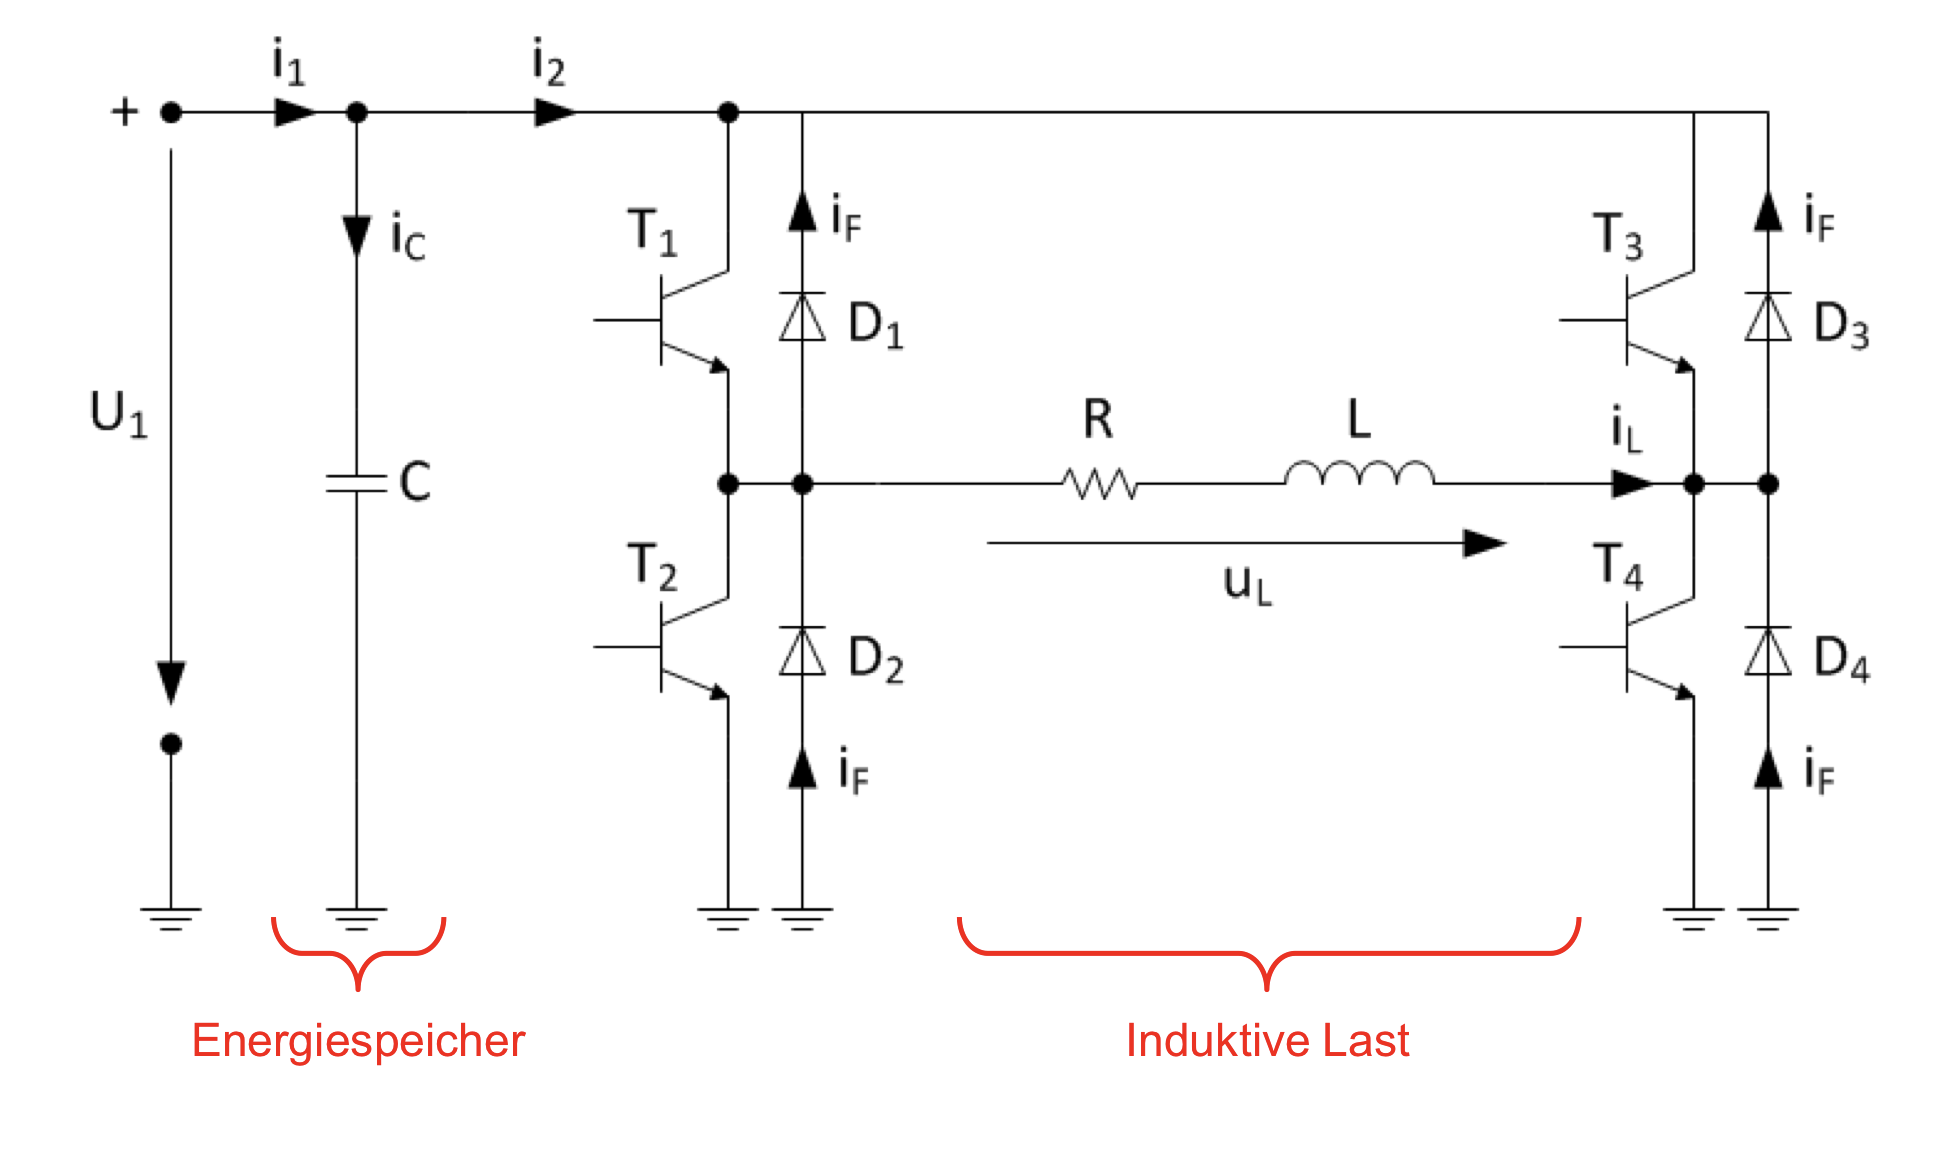
\includegraphics[width=0.85\linewidth]{images/1PWechselrichter.png}
\end{center}

Die H-Brücke besteht aus zwei Halbbrücken:
\begin{itemize}
\item obere Schalter $S_1, S_2$,
\item untere Schalter $S_3, S_4$.
\end{itemize}

Zulässige Schaltzustände:

\begin{center}
\begin{tabular}{c|c|c|c|c}
Zustand & $S_1$ & $S_2$ & $S_3$ & $S_4$ \\ \hline
$+U_{DC}$ & 1 & 0 & 0 & 1 \\
$-U_{DC}$ & 0 & 1 & 1 & 0 \\
Kurzschluss & 1 & 1 & 0 & 0 \\
Kurzschluss & 0 & 0 & 1 & 1 \\
\end{tabular}
\end{center}

\crd{\textrightarrow\ Obere und untere Schalter eines Zweigs dürfen nie gleichzeitig leiten (Shoot-Through).}

\subsection{Rechteckbetrieb (Grundbetrieb)}

Im einfachsten Fall wird die Brücke mit 50\,\% Tastgrad betrieben.

% --- bestehende Grafik: Zeitverlauf ---
\begin{center}
    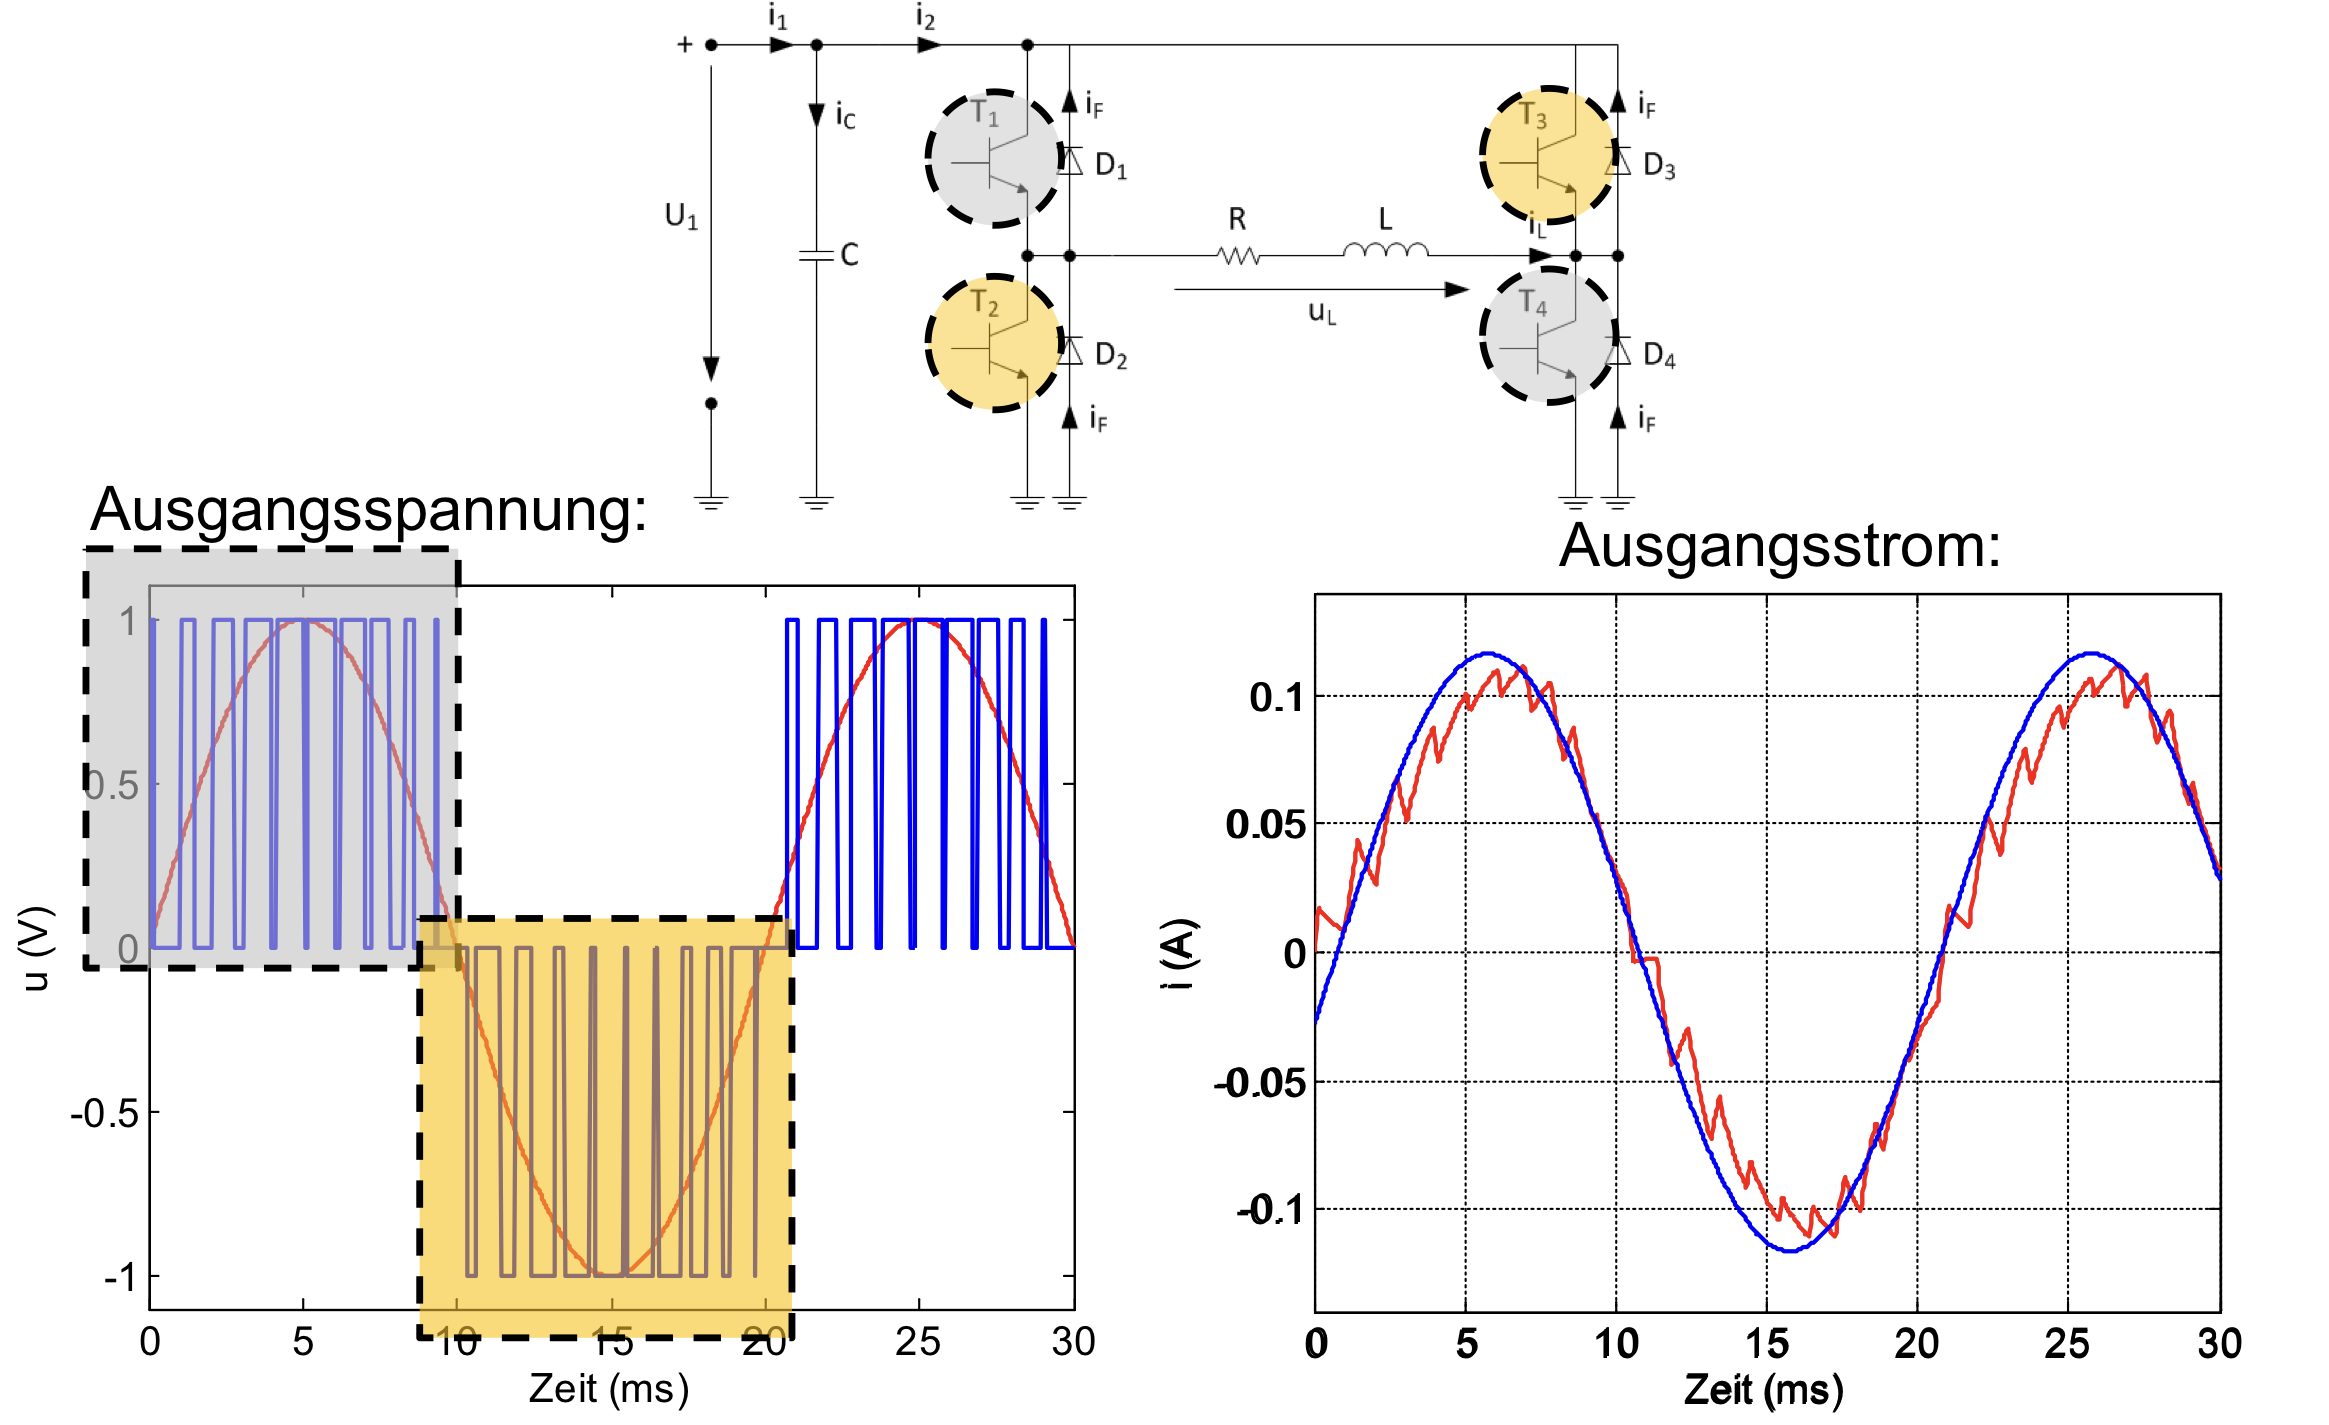
\includegraphics[width=0.85\linewidth]{images/1PWechselrichter_verlauf.png}
\end{center}

Ausgangsspannung:
\[
u_2(t) =
\begin{cases}
+U_{DC}, & 0 < \omega t < \pi \\
- U_{DC}, & \pi < \omega t < 2\pi
\end{cases}
\]

Frequenz:
\[
\boxed{f_2 = \frac{1}{T_2}}
\]

Amplitude:
\[
\boxed{\hat U = U_{DC}}
\]

\subsection{Fourier-Entwicklung des Rechtecksignals}

Fourier-Reihe:

\[
\boxed{
u_2(t) = \frac{4U_{DC}}{\pi} \left[
\sin(\omega t) + \frac{1}{3}\sin(3\omega t) + \frac{1}{5}\sin(5\omega t) + \ldots
\right]
}
\]

Grundschwingung:

\[
\boxed{\hat U_1 = \frac{4}{\pi} U_{DC}}
\]

Effektivwert der Grundschwingung:

\[
\boxed{U_{1,\mathrm{RMS}} = \frac{4}{\pi\sqrt{2}} U_{DC}}
\]

Konsequenzen:
\begin{itemize}
\item Nur ungerade Harmonische vorhanden.
\item Sehr hohe Verzerrung.
\item Keine Amplitudensteuerung möglich.
\end{itemize}

\subsection{Strom bei R--L-Last}

Bei induktiver Last gilt:
\[
i_2(t) = \frac{1}{L} \int u_2(t)\, dt
\]

Eigenschaften:
\begin{itemize}
\item Strom ist \textbf{phasenverschoben} zur Spannung.
\item Strom ist \textbf{glatter} als Spannung (Tiefpasswirkung der Induktivität).
\item Freilaufpfade sind zwingend erforderlich.
\end{itemize}

\subsection{PWM-Betrieb (Sinus-PWM)}

Zur Verbesserung der Spektraleigenschaften wird Pulsweitenmodulation eingesetzt.

Prinzip:
\begin{itemize}
\item Vergleich eines Sinus-Referenzsignals mit einem Dreieck-Trägersignal.
\item Schalter schalten mit hoher Frequenz $f_s$.
\item Grundschwingung folgt dem Sinus.
\end{itemize}

Ausgangsspannung:
\[
u_2(t) = \text{PWM-Signal mit Grundschwingung } u_{2,1}(t)
\]

Grundschwingungsamplitude:

\[
\boxed{\hat U_1 = m_a \frac{U_{DC}}{2}}, 
\qquad 0 \le m_a \le 1
\]

Effektivwert:

\[
\boxed{U_{1,\mathrm{RMS}} = m_a \frac{U_{DC}}{2\sqrt{2}}}
\]

\subsection{Spektrale Eigenschaften}

\subsubsection{Rechteckbetrieb}

\begin{itemize}
\item Nur ungerade Harmonische.
\item Harmonische bei $n = 3,5,7,\ldots$
\item Sehr hohe THD.
\end{itemize}

\subsubsection{PWM-Betrieb}

\begin{itemize}
\item Grundschwingung bei $f_2$.
\item Harmonische um Vielfache von $f_s$.
\item Tieffrequente Harmonische stark reduziert.
\item Filterung durch R--L-Last oder LC-Filter möglich.
\end{itemize}

\subsection{Leistungsfluss}

Momentanleistung:
\[
p(t) = u_2(t)\, i_2(t)
\]

Mittlere Leistung:
\[
\boxed{P = U_{1,\mathrm{RMS}} \, I_{1,\mathrm{RMS}} \cos\varphi_1}
\]

\begin{itemize}
\item Motorbetrieb: $P>0$.
\item Generatorbetrieb: $P<0$ (Rückspeisung möglich bei geeigneter Topologie).
\end{itemize}

\subsection{Typische Betriebsarten}

\begin{itemize}
\item Rechteckbetrieb: einfach, hohe Harmonische.
\item PWM-Betrieb: komplexer, gute Spannungsqualität.
\item Niedrige $f_s$: geringe Schaltverluste, schlechtere Filterbarkeit.
\item Hohe $f_s$: bessere Filterbarkeit, höhere Schaltverluste.
\end{itemize}

\subsection{Vergleich zu Gleichrichtern}

\begin{itemize}
\item Gleichrichter: AC $\rightarrow$ DC.
\item Wechselrichter: DC $\rightarrow$ AC.
\item Beide basieren auf identischer Brückentopologie.
\item Unterschied liegt nur in der Ansteuerung.
\end{itemize}

\subsection{Merksätze}

\begin{itemize}
\item H-Brücke erzeugt $\pm U_{DC}$ am Ausgang.
\item Rechteckbetrieb: keine Amplitudensteuerung, viele Harmonische.
\item PWM: Amplitude über $m_a$ steuerbar.
\item Induktive Last glättet den Strom.
\item Freilaufpfade sind zwingend notwendig.
\item Schaltfrequenz hoch $\Rightarrow$ Filter einfacher, Verluste grösser.
\end{itemize}

        \input{sections/11_Harmonische_Spektralanalyse.tex}
        \input{sections/12_PWM.tex}
        \section{Dreiphasiger Wechselrichter}

\subsection{Grundschaltung}

% --- bestehende Grafik: Dreiphasen-Brücke ---
\begin{center}
    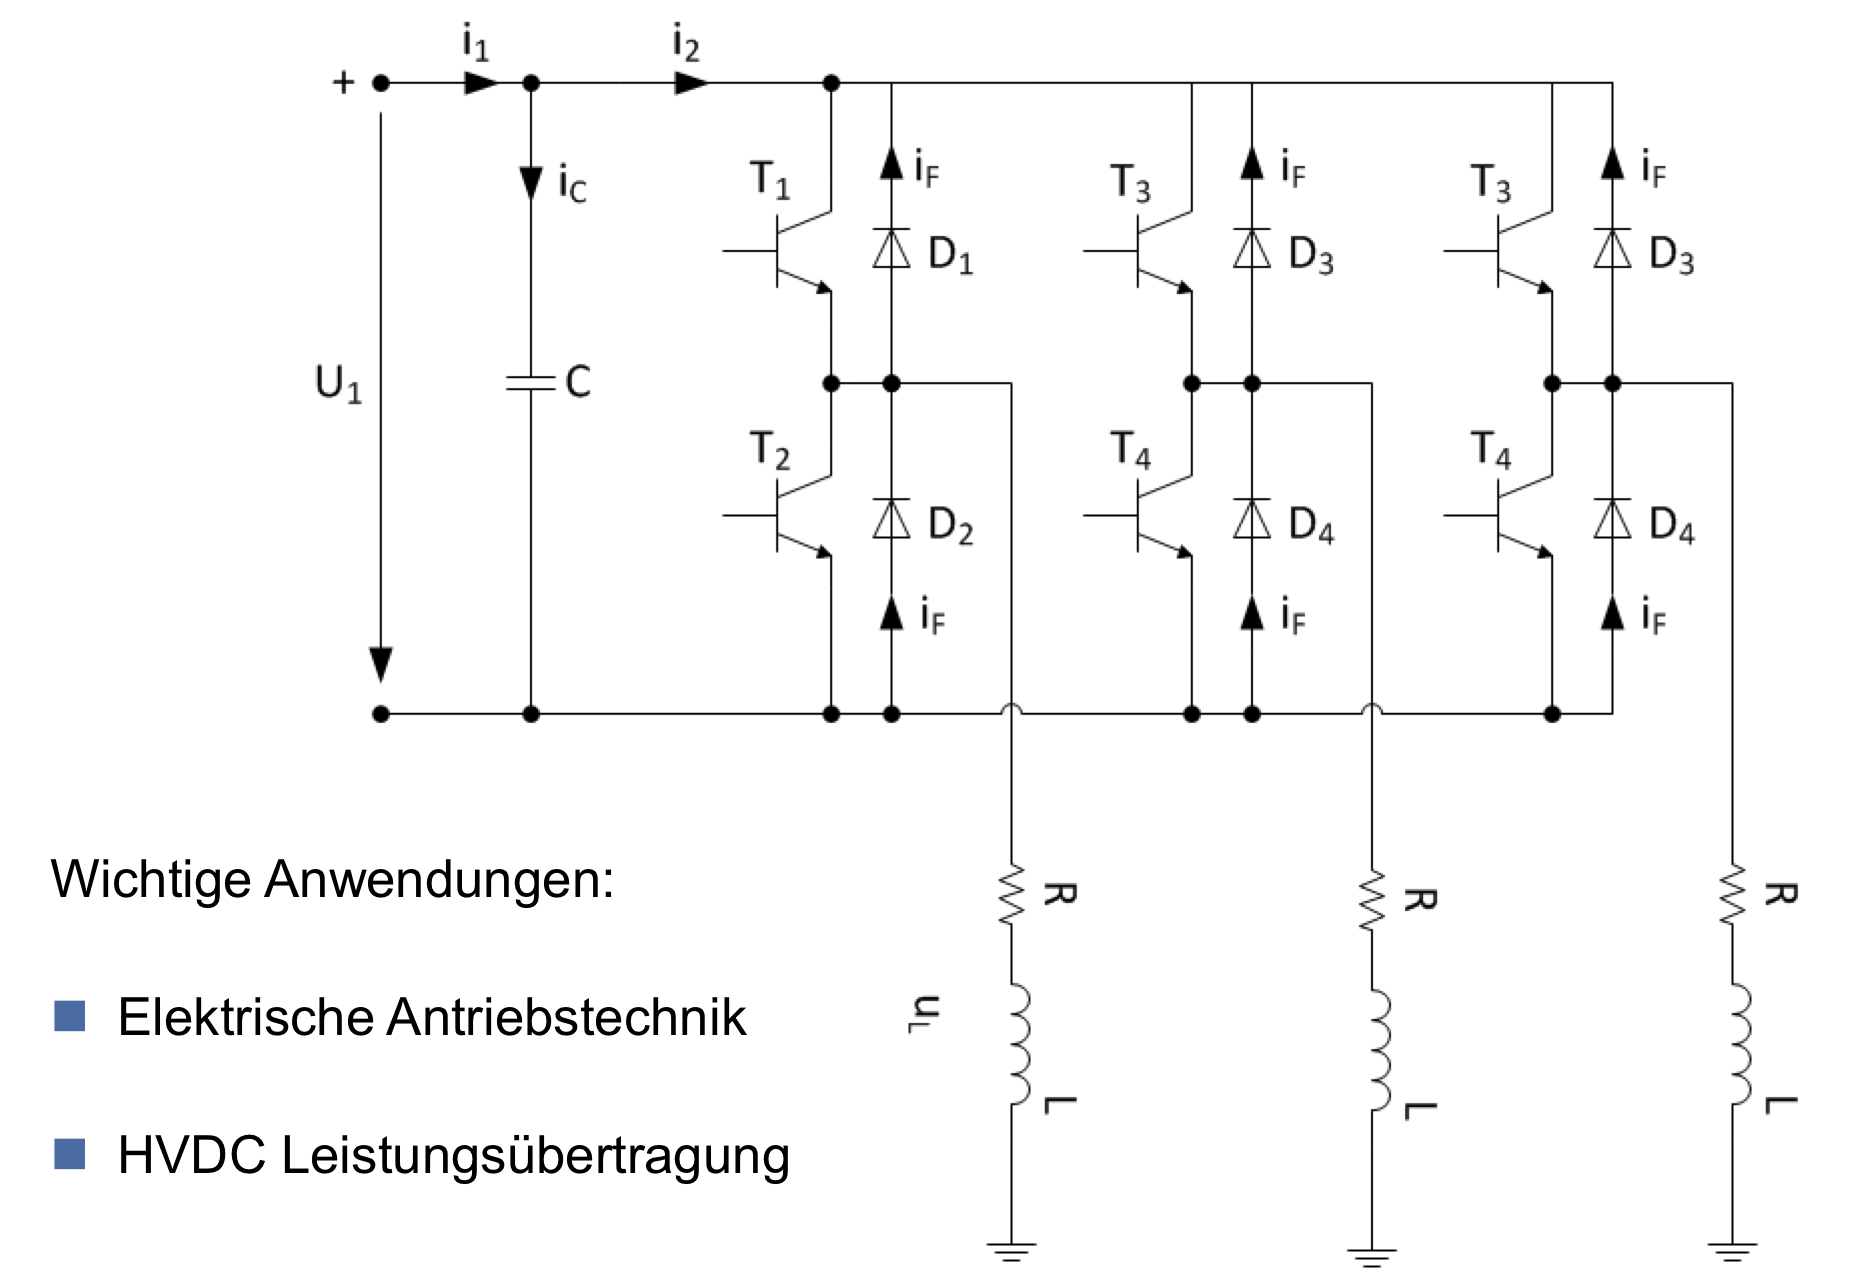
\includegraphics[width=0.85\linewidth]{images/3PWechselrichter.png}
\end{center}
Der dreiphasige Wechselrichter erzeugt aus $U_{DC}$ drei um $120^\circ$ phasenverschobene Spannungen.

\subsection{180$^\circ$-Betrieb}

% --- bestehende Grafik: 180 Grad Betrieb ---

Eigenschaften:
\begin{itemize}
    \item Jedes Ventil leitet 180$^\circ$
    \item Gute Ausnutzung der Gleichspannung
\end{itemize}

\subsection{120$^\circ$-Betrieb}


Eigenschaften:
\begin{itemize}
    \item Jedes Ventil leitet 120$^\circ$
    \item Geringere Schaltverluste
\end{itemize}

\subsection{Leiterspannungen und Grundschwingung}

Leiterspannung:
\[
\cbl{u_{LL} = u_a - u_b}
\]

Grundschwingungsamplitude:
\[
\cbl{\hat U_{LL,1} = \sqrt{3} \, \hat U_{ph,1}}
\]

\subsection{Vergleich Einphasig -- Dreiphasig}

\begin{center}
\begin{tabular}{l|c|c}
 & Einphasig & Dreiphasig \\ \hline
Phasen & 1 & \cbl{3} \\
Leistungsfluss & pulsierend & \cbl{konstant} \\
Oberschwingungen & hoch & \cbl{geringer} \\
\end{tabular}
\end{center}

\subsection{Merksätze}

\begin{itemize}
    \item PWM bestimmt Amplitude und Frequenz.
    \item 180$^\circ$- und 120$^\circ$-Betrieb unterscheiden sich in Leitintervallen.
    \item Dreiphasige Systeme liefern konstanten Leistungsfluss.
\end{itemize}


        \section{Direktumrichter}

Ein Direktumrichter wandelt eine Wechselspannung \textbf{direkt} in eine Wechselspannung
mit veränderlicher Frequenz und Amplitude, \textbf{ohne Zwischenkreis}.

\subsection{Grundprinzip}

\begin{center}
    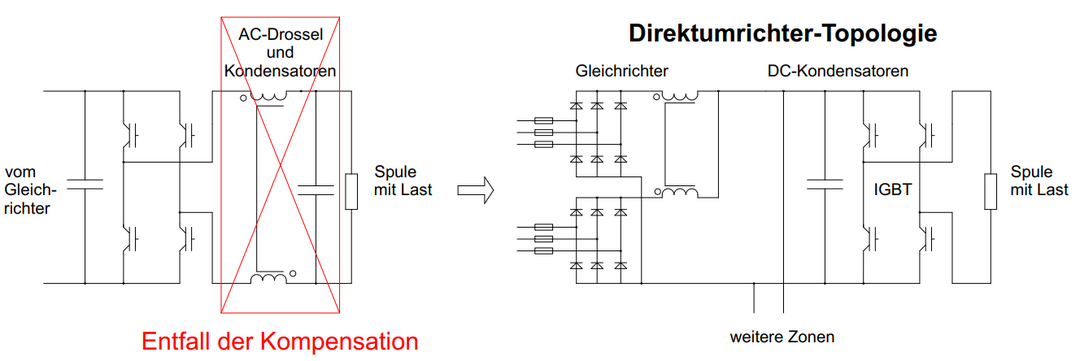
\includegraphics[width=0.85\linewidth]{images/direktumrichtergrund.png}
\end{center}

Eigenschaften:
\begin{itemize}
    \item Keine Gleichstrom-Zwischenstufe
    \item Direkte AC-AC-Wandlung
    \item Ausgangsfrequenz kleiner als Eingangsfrequenz
\end{itemize}

\crd{\textrightarrow\ Direktumrichter sind direkte AC-AC-Umrichter ohne Energiespeicher.}

% -------------------------------------------------
\subsection{Leistungsfluss und Vierquadrantenbetrieb}

\[
\boxed{P = u_2(t)\, i_2(t)}
\]

Direktumrichter erlauben:
\begin{itemize}
\item Motorbetrieb,
\item Generatorbetrieb,
\item Rückspeisung ins Netz.
\end{itemize}

Sie sind grundsätzlich vierquadrantenfähig.


\subsection{Schaltungsstruktur}

\begin{center}
    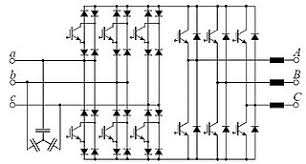
\includegraphics[width=0.85\linewidth]{images/direktumrichter_matrix.png}
\end{center}

Ein Direktumrichter besteht aus einer Matrix von bidirektionalen Schaltern,
die jede Eingangsphase mit jeder Ausgangsphase verbinden können.

Anzahl der Schalter:
\[
\cbl{3 \times 3 = 9 \text{ bidirektionale Schalter}}
\]

\subsection{Frequenzbereich}

\[
\cbl{f_2 < \frac{1}{2} f_1}
\]

Aussage:
\begin{itemize}
    \item Ausgangsfrequenz ist kleiner als Netzfrequenz
    \item Begrenzung durch Kommutierungsbedingungen
\end{itemize}

% -------------------------------------------------

\subsection{Kommutierung}

\begin{center}
    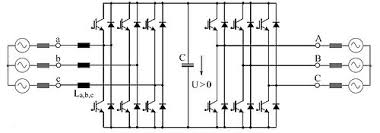
\includegraphics[width=0.85\linewidth]{images/direktumrichter_kommutierung.png}
\end{center}

Bei der Kommutierung darf \textbf{keine Netzphase kurzgeschlossen} und
\textbf{keine Lastphase unterbrochen} werden.

Grundregeln:
\begin{itemize}
    \item Niemals zwei Netzphasen kurzschliessen
    \item Niemals Laststrom unterbrechen
\end{itemize}

\crd{\textrightarrow\ Kommutierung ist das Hauptproblem des Direktumrichters.}

% -------------------------------------------------

\subsection{Eigenschaften und Einordnung}

\begin{itemize}
    \item Sehr robuste Industrieumrichter
    \item Hoher Wirkungsgrad
    \item Komplexe Steuerung
\end{itemize}

\subsection{Vergleich Direktumrichter -- Wechselrichter}

\begin{center}
\begin{tabular}{l|c|c}
 & Direktumrichter & Wechselrichter \\ \hline
Zwischenkreis & nein & \cbl{ja} \\
Eingang & AC & AC/DC \\
Ausgang & AC & AC \\
Frequenzbereich & $f_2 < \frac{1}{2}f_1$ & \cbl{frei wählbar} \\
\end{tabular}
\end{center}

\subsection{Merksätze}

\begin{itemize}
    \item Direktumrichter sind direkte AC-AC-Umrichter.
    \item Keine Zwischenkreisspannung vorhanden.
    \item Ausgangsfrequenz ist begrenzt.
\end{itemize}

        \input{sections/100_fourierreihen.tex}
        \section{Mathematische Analyse -- Formelsammlung}

Diese Section sammelt die \textbf{wichtigsten mathematischen Werkzeuge}
für die Analyse in der Leistungselektronik:
\textbf{Ableitungen}, \textbf{Integrale}, \textbf{Trigonometrie},
\textbf{Exponentialfunktionen}, \textbf{Komplexrechnung},
\textbf{Laplace-Transformation} und \textbf{Differentialgleichungen (RLC)}.
Sie ist als \textbf{reine Nachschlage-Section} gedacht.

\smallskip

\textbf{Ziel:}
\begin{itemize}
    \item Schneller Zugriff auf Standardformeln
    \item Fehlerfreie Umformungen in Prüfungen
    \item Einheitliche Notation im ganzen Skript
\end{itemize}

% -------------------------------------------------
\subsection{Grundlegende Ableitungsregeln}

\subsubsection{Elementare Funktionen}

\[
\frac{d}{dx} c = 0
\qquad
\frac{d}{dx} x = 1
\qquad
\frac{d}{dx} x^n = n x^{n-1}
\]

\[
\frac{d}{dx} \e^{x} = \e^{x}
\qquad
\frac{d}{dx} \ln x = \frac{1}{x}
\]

\subsubsection{Lineare Regeln}

\[
\frac{d}{dx} [f(x) + g(x)] = f'(x) + g'(x)
\qquad
\frac{d}{dx} [c \, f(x)] = c \, f'(x)
\]

\subsubsection{Produktregel}

\[
\cbl{\frac{d}{dx} [f(x) g(x)] = f'(x) g(x) + f(x) g'(x)}
\]

\subsubsection{Quotientenregel}

\[
\cbl{\frac{d}{dx} \left[ \frac{f(x)}{g(x)} \right]
= \frac{f'(x) g(x) - f(x) g'(x)}{g(x)^2}}
\]

\subsubsection{Kettenregel}

\[
\cbl{\frac{d}{dx} f(g(x)) = f'(g(x)) \cdot g'(x)}
\]

% -------------------------------------------------
\subsection{Ableitungen trigonometrischer Funktionen}

\[
\cbl{\frac{d}{dx} \sin x = \cos x}
\qquad
\cbl{\frac{d}{dx} \cos x = - \sin x}
\]

\[
\frac{d}{dx} \tan x = \frac{1}{\cos^2 x}
\qquad
\frac{d}{dx} \cot x = - \frac{1}{\sin^2 x}
\]

\[
\frac{d}{dx} \arcsin x = \frac{1}{\sqrt{1-x^2}}
\qquad
\frac{d}{dx} \arccos x = -\frac{1}{\sqrt{1-x^2}}
\]

% -------------------------------------------------
\subsection{Grundlegende Integralregeln}

\subsubsection{Elementare Integrale}

\[
\int c \, dx = c x + C
\qquad
\int x^n \, dx = \frac{x^{n+1}}{n+1} + C \quad (n \neq -1)
\]

\[
\int \frac{1}{x} \, dx = \ln |x| + C
\qquad
\int \e^{x} \, dx = \e^{x} + C
\]

\subsubsection{Lineare Regeln}

\[
\int [f(x) + g(x)] dx = \int f(x) dx + \int g(x) dx
\qquad
\int c f(x) dx = c \int f(x) dx
\]

% -------------------------------------------------
\subsection{Integrale trigonometrischer Funktionen}

\[
\cbl{\int \sin x \, dx = - \cos x + C}
\qquad
\cbl{\int \cos x \, dx = \sin x + C}
\]

\[
\int \tan x \, dx = - \ln |\cos x| + C
\qquad
\int \cot x \, dx = \ln |\sin x| + C
\]

\[
\int \sin^2 x \, dx = \frac{x}{2} - \frac{\sin(2x)}{4} + C
\qquad
\int \cos^2 x \, dx = \frac{x}{2} + \frac{\sin(2x)}{4} + C
\]

\[
\int \sin(ax) \, dx = -\frac{1}{a}\cos(ax) + C
\qquad
\int \cos(ax) \, dx = \frac{1}{a}\sin(ax) + C
\]

% -------------------------------------------------
\subsection{Partielle Integration}

\[
\cbl{\int u \, dv = u v - \int v \, du}
\]

Beispiel:
\[
\int x \e^{x} dx = x \e^{x} - \int \e^{x} dx = (x-1) \e^{x} + C
\]

% -------------------------------------------------
\subsection{Substitution}

\[
\cbl{u = g(x), \qquad du = g'(x) dx}
\]

Beispiel:
\[
\int \sin(3x) dx
= -\frac{1}{3} \cos(3x) + C
\]

% -------------------------------------------------
\subsection{Trigonometrische Identitäten}

\subsubsection{Grundidentitäten}

\[
\cbl{\sin^2 x + \cos^2 x = 1}
\qquad
\cbl{1 + \tan^2 x = \frac{1}{\cos^2 x}}
\qquad
1 + \cot^2 x = \frac{1}{\sin^2 x}
\]

\subsubsection{Winkeladdition}

\[
\cbl{\sin(a \pm b) = \sin a \cos b \pm \cos a \sin b}
\]

\[
\cbl{\cos(a \pm b) = \cos a \cos b \mp \sin a \sin b}
\]

\subsubsection{Doppelwinkel}

\[
\cbl{\sin(2x) = 2 \sin x \cos x}
\qquad
\cbl{\cos(2x) = \cos^2 x - \sin^2 x = 1 - 2 \sin^2 x = 2 \cos^2 x - 1}
\]

\subsubsection{Halbwinkel}

\[
\cbl{\sin^2\left(\frac{x}{2}\right) = \frac{1-\cos x}{2}}
\qquad
\cbl{\cos^2\left(\frac{x}{2}\right) = \frac{1+\cos x}{2}}
\]

% -------------------------------------------------
\subsection{Produkt--Summen--Formeln}

\[
\cbl{\sin a \cos b = \frac{1}{2} [ \sin(a+b) + \sin(a-b) ]}
\]

\[
\cbl{\cos a \cos b = \frac{1}{2} [ \cos(a+b) + \cos(a-b) ]}
\]

\[
\cbl{\sin a \sin b = \frac{1}{2} [ \cos(a-b) - \cos(a+b) ]}
\]

\[
\cbl{\sin a + \sin b = 2 \sin\left(\frac{a+b}{2}\right) \cos\left(\frac{a-b}{2}\right)}
\]

\[
\cbl{\cos a + \cos b = 2 \cos\left(\frac{a+b}{2}\right) \cos\left(\frac{a-b}{2}\right)}
\]

\[
\cbl{\cos a - \cos b = -2 \sin\left(\frac{a+b}{2}\right) \sin\left(\frac{a-b}{2}\right)}
\]

% -------------------------------------------------
\subsection{Exponential- und Euler-Formeln}

\subsubsection{Euler-Formel}

\[
\cbl{\e^{\jimg x} = \cos x + \jimg \sin x}
\qquad
\cbl{\e^{-\jimg x} = \cos x - \jimg \sin x}
\]

\[
\cbl{\cos x = \frac{\e^{\jimg x} + \e^{-\jimg x}}{2}}
\qquad
\cbl{\sin x = \frac{\e^{\jimg x} - \e^{-\jimg x}}{2\jimg}}
\]

\subsubsection{Komplexe Sinusdarstellung}

\[
\cbl{\hat X \sin(\omega t + \varphi) = \Im\left\{ \hat X \e^{\jimg(\omega t + \varphi)} \right\}}
\]

\[
\cbl{\hat X \cos(\omega t + \varphi) = \Re\left\{ \hat X \e^{\jimg(\omega t + \varphi)} \right\}}
\]

% -------------------------------------------------
\subsection{Komplexrechnung}

\subsubsection{Grundformen}

\[
\cbl{z = x + \jimg y}
\qquad
\cbl{z = r \e^{\jimg \varphi}}
\]

\[
r = |z| = \sqrt{x^2 + y^2}
\qquad
\varphi = \arg(z)
\]

\subsubsection{Konjugation}

\[
\cbl{\overline{z} = x - \jimg y}
\qquad
\cbl{z \overline{z} = |z|^2}
\]

\subsubsection{Multiplikation und Division}

\[
\cbl{z_1 z_2 = r_1 r_2 \e^{\jimg (\varphi_1 + \varphi_2)}}
\qquad
\cbl{\frac{z_1}{z_2} = \frac{r_1}{r_2} \e^{\jimg (\varphi_1 - \varphi_2)}}
\]

\subsubsection{Real- und Imaginärteil}

\[
\cbl{\Re(z) = x}
\qquad
\cbl{\Im(z) = y}
\]

% -------------------------------------------------
\subsection{Komplexe Wechselstromrechnung}

\subsubsection{Ableiten im Zeitbereich}

\[
\cbl{\frac{d}{dt} \e^{\jimg \omega t} = \jimg \omega \e^{\jimg \omega t}}
\]

\subsubsection{Impedanzen}

\[
\cbl{Z_R = R}
\qquad
\cbl{Z_L = \jimg \omega L}
\qquad
\cbl{Z_C = \frac{1}{\jimg \omega C}}
\]

\subsubsection{Serien- und Parallelschaltung}

\[
\cbl{Z_{\mathrm{Serie}} = Z_1 + Z_2 + \dots}
\]

\[
\cbl{\frac{1}{Z_{\mathrm{Par}}} = \frac{1}{Z_1} + \frac{1}{Z_2} + \dots}
\]

% -------------------------------------------------
\subsection{Orthogonalitätsintegrale (Fourier-Kern)}

\[
\cbl{\int_0^T \cos(m \omega t)\cos(n \omega t)\,dt =
\begin{cases}
T, & m=n=0 \\
\frac{T}{2}, & m=n>0 \\
0, & m\neq n
\end{cases}}
\]

\[
\cbl{\int_0^T \sin(m \omega t)\sin(n \omega t)\,dt =
\begin{cases}
\frac{T}{2}, & m=n \\
0, & m\neq n
\end{cases}}
\]

\[
\cbl{\int_0^T \sin(m \omega t)\cos(n \omega t)\,dt = 0}
\]

% -------------------------------------------------
\subsection{Grenzwerte und Reihen}

\[
\cbl{\lim_{x \to 0} \frac{\sin x}{x} = 1}
\qquad
\cbl{\lim_{x \to 0} \frac{1 - \cos x}{x^2} = \frac{1}{2}}
\]

\[
\cbl{\e^{x} = \sum_{n=0}^{\infty} \frac{x^n}{n!}}
\qquad
\cbl{\sin x = \sum_{n=0}^{\infty} (-1)^n \frac{x^{2n+1}}{(2n+1)!}}
\qquad
\cbl{\cos x = \sum_{n=0}^{\infty} (-1)^n \frac{x^{2n}}{(2n)!}}
\]

% -------------------------------------------------
\subsection{Bestimmte Integrale über Perioden}

\[
\cbl{\int_0^T \sin(n \omega t)\,dt = 0}
\qquad
\cbl{\int_0^T \cos(n \omega t)\,dt = 0}
\]

\[
\cbl{\int_0^T \sin^2(n \omega t)\,dt = \frac{T}{2}}
\qquad
\cbl{\int_0^T \cos^2(n \omega t)\,dt = \frac{T}{2}}
\]

% =================================================
\subsection{Laplace-Transformation}

\subsubsection{Definition}

Für eine zeitkontinuierliche Funktion $f(t)$ (typisch $t\ge 0$):
\[
\cbl{\mathcal{L}\{f(t)\} = F(s) = \int_{0}^{\infty} f(t)\, \e^{-st}\,dt}
\qquad
s = \sigma + \jimg \omega
\]

\subsubsection{Wichtige Grundtransformierte}

\[
\mathcal{L}\{1\} = \frac{1}{s}
\qquad
\mathcal{L}\{t\} = \frac{1}{s^2}
\qquad
\mathcal{L}\{t^n\} = \frac{n!}{s^{n+1}}
\]

\[
\cbl{\mathcal{L}\{\e^{at}\} = \frac{1}{s-a}}
\]

\[
\cbl{\mathcal{L}\{\sin(\omega t)\} = \frac{\omega}{s^2+\omega^2}}
\qquad
\cbl{\mathcal{L}\{\cos(\omega t)\} = \frac{s}{s^2+\omega^2}}
\]

\[
\mathcal{L}\{\sinh(\omega t)\} = \frac{\omega}{s^2-\omega^2}
\qquad
\mathcal{L}\{\cosh(\omega t)\} = \frac{s}{s^2-\omega^2}
\]

\subsubsection{Linearität}

\[
\cbl{\mathcal{L}\{a f(t) + b g(t)\} = aF(s) + bG(s)}
\]

\subsubsection{Ableitungssatz}

\[
\cbl{\mathcal{L}\left\{\frac{df}{dt}\right\} = sF(s) - f(0)}
\]

\[
\cbl{\mathcal{L}\left\{\frac{d^2f}{dt^2}\right\} = s^2F(s) - s f(0) - f'(0)}
\]

\crd{\textrightarrow\ Anfangswerte gehen als Terme in den Zähler. Häufige Prüfungsfalle.}

\subsubsection{Integralsatz}

\[
\cbl{\mathcal{L}\left\{\int_0^t f(\tau)\,d\tau\right\} = \frac{1}{s} F(s)}
\]

\subsubsection{Zeitverschiebung (Heaviside)}

\[
\cbl{\mathcal{L}\{f(t-t_0)u(t-t_0)\} = \e^{-s t_0} F(s)}
\]

\subsubsection{Frequenzverschiebung}

\[
\cbl{\mathcal{L}\{\e^{at} f(t)\} = F(s-a)}
\]

\subsubsection{Faltung}

\[
\cbl{(f*g)(t) = \int_0^t f(\tau)g(t-\tau)\,d\tau}
\qquad
\cbl{\mathcal{L}\{f*g\} = F(s)G(s)}
\]

\subsubsection{Initial- und Finalwertsatz}

\[
\cbl{f(0^+) = \lim_{s\to\infty} sF(s)}
\qquad
\cbl{f(\infty) = \lim_{s\to 0} sF(s)}
\]

\crd{\textrightarrow\ Finalwertsatz nur gültig, wenn alle Pole von $sF(s)$ in der linken Halbebene liegen.}

\subsubsection{Inverse Laplace (Standardstrategien)}

\begin{itemize}
    \item Partialbruchzerlegung
    \item Tabellenrücktransformation
    \item Verschiebungssätze (Zeit, Frequenz)
    \item Quadratische Ergänzung für $s^2+\omega^2$
\end{itemize}

% =================================================
\subsection{Übertragungsfunktionen und Systemdarstellung}

Für lineare zeitinvariante Systeme (LTI):
\[
\cbl{H(s) = \frac{Y(s)}{X(s)}}
\]

\subsubsection{Pol-Nullstellen-Darstellung}

\[
\cbl{H(s)=K \frac{(s-z_1)(s-z_2)\dots}{(s-p_1)(s-p_2)\dots}}
\]

\subsubsection{Zeitkonstante und Eckfrequenz}

Erste Ordnung:
\[
\cbl{H(s)=\frac{1}{1+s\tau}}
\qquad
\cbl{\omega_c = \frac{1}{\tau}}
\qquad
\cbl{f_c = \frac{1}{2\pi\tau}}
\]

% =================================================
\subsection{Differentialgleichungen 1. Ordnung (R--L / R--C)}

\subsubsection{Standardform}

\[
\cbl{\tau \frac{dy}{dt} + y = K \, u(t)}
\]

Homogene Lösung:
\[
\cbl{y_h(t) = C \e^{-t/\tau}}
\]

Partikuläre Lösung (Konstantanregung $u(t)=U$):
\[
\cbl{y_p(t)=K U}
\]

Gesamtlösung:
\[
\cbl{y(t) = K U + \big(y(0)-K U\big)\e^{-t/\tau}}
\]

\subsubsection{R--L-Kreis}

\[
\cbl{L\frac{di}{dt} + Ri = u(t)}
\qquad
\cbl{\tau = \frac{L}{R}}
\]

Sprung $u(t)=U$:
\[
\cbl{i(t) = \frac{U}{R}\left(1-\e^{-t/\tau}\right) + i(0)\e^{-t/\tau}}
\]

\subsubsection{R--C-Kreis}

\[
\cbl{RC\frac{du_C}{dt} + u_C = u(t)}
\qquad
\cbl{\tau = RC}
\]

Sprung $u(t)=U$:
\[
\cbl{u_C(t) = U\left(1-\e^{-t/\tau}\right) + u_C(0)\e^{-t/\tau}}
\]

\crd{\textrightarrow\ Bei Induktivitäten ist $i(t)$ stetig, bei Kapazitäten ist $u_C(t)$ stetig.}

% =================================================
\subsection{Differentialgleichungen 2. Ordnung (RLC-Systeme)}

\subsubsection{Standardform}

\[
\cbl{\frac{d^2y}{dt^2} + 2\zeta\omega_0 \frac{dy}{dt} + \omega_0^2 y = K \omega_0^2 u(t)}
\]

\[
\cbl{\omega_0 = \sqrt{\frac{1}{LC}}}
\qquad
\cbl{\zeta = \frac{R}{2}\sqrt{\frac{C}{L}}}
\]

\subsubsection{Dämpfungsfälle}

\begin{itemize}
    \item \textbf{Unterdämpft:} $0<\zeta<1$ (schwingend)
    \item \textbf{Kritisch gedämpft:} $\zeta=1$
    \item \textbf{Überdämpft:} $\zeta>1$
\end{itemize}

Unterdämpfte Eigenfrequenz:
\[
\cbl{\omega_d = \omega_0\sqrt{1-\zeta^2}}
\]

\subsubsection{Freie Schwingung (homogene Lösung)}

Unterdämpft:
\[
\cbl{y_h(t)=\e^{-\zeta\omega_0 t}\left(C_1\cos(\omega_d t)+C_2\sin(\omega_d t)\right)}
\]

Überdämpft:
\[
\cbl{y_h(t)=C_1\e^{s_1 t}+C_2\e^{s_2 t}}
\qquad
s_{1,2}=-\omega_0\left(\zeta\pm\sqrt{\zeta^2-1}\right)
\]

Kritisch:
\[
\cbl{y_h(t)=(C_1 + C_2 t)\e^{-\omega_0 t}}
\]

\subsubsection{Serien-RLC (Stromdynamik)}

KVL:
\[
\cbl{u(t)=Ri(t)+L\frac{di}{dt}+\frac{1}{C}\int i(t)\,dt}
\]

Differenziert:
\[
\cbl{\frac{d^2 i}{dt^2} + \frac{R}{L}\frac{di}{dt} + \frac{1}{LC}i = \frac{1}{L}\frac{du}{dt}}
\]

\subsubsection{Parallele-RLC (Spannungsdynamik)}

KCL:
\[
i(t)=\frac{u(t)}{R}+C\frac{du}{dt}+\frac{1}{L}\int u(t)\,dt
\]

Differenziert:
\[
\cbl{\frac{d^2 u}{dt^2} + \frac{1}{RC}\frac{du}{dt} + \frac{1}{LC}u = \frac{1}{C}\frac{di}{dt}}
\]

\subsubsection{Laplace-Lösung von DGLs}

Vorgehen:
\begin{enumerate}
    \item DGL aufstellen (KVL/KCL)
    \item Laplace anwenden (Ableitungssätze)
    \item Nach $Y(s)$ auflösen
    \item Partialbrüche
    \item Rücktransformation
\end{enumerate}

\subsubsection{Standardübertragungsfunktionen}

\paragraph{Tiefpass 1. Ordnung}
\[
\cbl{H(s)=\frac{1}{1+s\tau}}
\]

\paragraph{Bandpass / Resonanz 2. Ordnung (Normalform)}
\[
\cbl{H(s)=\frac{\omega_0^2}{s^2+2\zeta\omega_0 s+\omega_0^2}}
\]

% -------------------------------------------------
\subsection{Typische Merksätze (Analyse-Kern)}

\begin{itemize}
    \item Kettenregel, Produktregel, trigonometrische Identitäten sicher beherrschen.
    \item Laplace macht aus DGLs algebraische Gleichungen.
    \item $i_L(t)$ und $u_C(t)$ sind stetig.
    \item Polstellen bestimmen Stabilität und Zeitverhalten.
\end{itemize}

\subsection{Typische Fehlerquellen}

\begin{itemize}
    \item Anfangswerte bei Laplace-Ableitung vergessen.
    \item Finalwertsatz ohne Polprüfung verwendet.
    \item Vorzeichenfehler bei $\cos'(x)$ und bei KVL/KCL.
    \item $u_C$ bzw. $i_L$ als sprungfähig angenommen.
\end{itemize}

        \input{sections/300_ETformeln.tex}
        \section{Lösen von Differentialgleichungen}

Diese Section zeigt ein \textbf{systematisches Vorgehen} zum Lösen typischer
Differentialgleichungen in der Elektrotechnik und Leistungselektronik.
Fokus: \textbf{1. Ordnung} (R--L / R--C) und \textbf{2. Ordnung} (RLC),
inkl. \textbf{Stückweise-Betrieb} (Schaltzustände), wie er bei Umrichtern ständig vorkommt.

\smallskip

\textbf{Zielbild:}
\begin{itemize}
    \item DGL-Typ schnell erkennen
    \item Standardlösung aufbauen (homogen + particular)
    \item Anfangs- und Randbedingungen korrekt einsetzen
    \item Laplace-Methode sicher anwenden
    \item Stückweise Lösungen sauber verketten
\end{itemize}

% -------------------------------------------------
\subsection{DGL-Typen (Prüfungs-Screening)}

\subsubsection{1. Ordnung (typisch R--L, R--C)}

\[
\cbl{a \frac{dy}{dt} + b y = g(t)}
\]

\subsubsection{2. Ordnung (typisch RLC, mechanische Systeme)}

\[
\cbl{a \frac{d^2y}{dt^2} + b \frac{dy}{dt} + c y = g(t)}
\]

\subsubsection{Stückweise DGL (Umrichterbetrieb)}

\[
\cbl{\text{Je Schaltzustand eigene DGL, dann Übergangsbedingungen.}}
\]

\crd{\textrightarrow\ 80\% der Punkte kommen aus sauberem Strukturieren, nicht aus Rechenkunst.}

% -------------------------------------------------
\subsection{Universales Vorgehen}

\begin{enumerate}
    \item \textbf{Signal und System definieren:} gesuchte Grösse $y(t)$, Eingänge, Parameter.
    \item \textbf{DGL aufstellen:} KVL/KCL oder Energie-/Kraftgleichungen.
    \item \textbf{DGL normieren:} auf Standardform bringen.
    \item \textbf{Lösungsansatz wählen:}
    \begin{itemize}
        \item Zeitbereich (homogen + particular)
        \item Laplace (algebraisch)
    \end{itemize}
    \item \textbf{Konstanten bestimmen:} Anfangswerte, Periodenbedingungen, Randbedingungen.
    \item \textbf{Plausibilisieren:} Grenzfälle $t\to 0$, $t\to\infty$, Einheiten, Vorzeichen.
\end{enumerate}

% -------------------------------------------------
\subsection{DGL 1. Ordnung im Zeitbereich}

\subsubsection{Standardform}

\[
\cbl{\frac{dy}{dt} + \frac{1}{\tau} y = k \, u(t)}
\qquad
\cbl{\tau = \frac{a}{b}}
\]

\subsubsection{Lösungsstruktur}

\[
\cbl{y(t) = y_h(t) + y_p(t)}
\]

Homogene Lösung ($u(t)=0$):
\[
\cbl{y_h(t) = C \e^{-t/\tau}}
\]

Partikuläre Lösung hängt von $u(t)$ ab.

\subsubsection{Wichtiger Spezialfall: Konstantanregung $u(t)=U$}

Partikulär:
\[
\cbl{y_p = k U \tau \cdot \frac{1}{\tau} = kU}
\]

Gesamtlösung:
\[
\cbl{y(t) = kU + \big(y(0)-kU\big)\e^{-t/\tau}}
\]

\crd{\textrightarrow\ Merksatz: Endwert + (Start-Endwert)$\cdot e^{-t/\tau}$.}

% -------------------------------------------------
\subsection{Beispiel 1: R--L-Kreis (Stromanstieg)}

KVL:
\[
\cbl{L\frac{di}{dt} + Ri = U}
\qquad
\Rightarrow
\qquad
\frac{di}{dt} + \frac{R}{L} i = \frac{U}{L}
\]

Zeitkonstante:
\[
\cbl{\tau = \frac{L}{R}}
\]

Lösung:
\[
\cbl{i(t) = \frac{U}{R} + \left(i(0) - \frac{U}{R}\right)\e^{-t/\tau}}
\]

Spezialfall $i(0)=0$:
\[
\cbl{i(t) = \frac{U}{R}\left(1-\e^{-t/\tau}\right)}
\]

% -------------------------------------------------
\subsection{Beispiel 2: R--C-Kreis (Spannungsanstieg am Kondensator)}

KVL:
\[
\cbl{u_R + u_C = U,\quad u_R = Ri,\quad i = C\frac{du_C}{dt}}
\]

\[
RC\frac{du_C}{dt}+u_C = U
\qquad
\cbl{\tau = RC}
\]

Lösung:
\[
\cbl{u_C(t) = U + \big(u_C(0)-U\big)\e^{-t/\tau}}
\]

Spezialfall $u_C(0)=0$:
\[
\cbl{u_C(t) = U\left(1-\e^{-t/\tau}\right)}
\]

% -------------------------------------------------
\subsection{Integrierender Faktor (allgemeine 1. Ordnung)}

Für:
\[
\cbl{\frac{dy}{dt} + p(t) y = q(t)}
\]

Integrierender Faktor:
\[
\cbl{\mu(t) = \e^{\int p(t)\,dt}}
\]

Dann:
\[
\cbl{y(t) = \frac{1}{\mu(t)}\left(\int \mu(t) q(t)\,dt + C\right)}
\]

% -------------------------------------------------
\subsection{DGL 2. Ordnung im Zeitbereich}

\subsubsection{Standardform}

\[
\cbl{\frac{d^2y}{dt^2} + 2\zeta\omega_0 \frac{dy}{dt} + \omega_0^2 y = K\omega_0^2 u(t)}
\]

Parameter:
\[
\cbl{\omega_0 = \sqrt{\frac{1}{LC}}}
\qquad
\cbl{\zeta = \frac{R}{2}\sqrt{\frac{C}{L}}}
\]

\subsubsection{Homogene Lösung über charakteristische Gleichung}

Ansatz:
\[
y_h(t)=\e^{st}
\]

Charakteristische Gleichung:
\[
\cbl{s^2 + 2\zeta\omega_0 s + \omega_0^2 = 0}
\]

Pole:
\[
\cbl{s_{1,2} = -\zeta\omega_0 \pm \omega_0\sqrt{\zeta^2-1}}
\]

\subsubsection{Fälle}

Unterdämpft ($0<\zeta<1$):
\[
\cbl{y_h(t)=\e^{-\zeta\omega_0 t}\left(C_1\cos(\omega_d t)+C_2\sin(\omega_d t)\right)}
\]
\[
\cbl{\omega_d = \omega_0\sqrt{1-\zeta^2}}
\]

Kritisch ($\zeta=1$):
\[
\cbl{y_h(t)=(C_1+C_2 t)\e^{-\omega_0 t}}
\]

Überdämpft ($\zeta>1$):
\[
\cbl{y_h(t)=C_1\e^{s_1 t}+C_2\e^{s_2 t}}
\]

\subsubsection{Partikuläre Lösung}

Typische Prüfungsinputs:
\begin{itemize}
    \item Konstante $u(t)=U$
    \item Sprung $u(t)=U\cdot 1(t)$
    \item Sinus $u(t)=\hat U\sin(\omega t)$ (Frequenzantwort)
\end{itemize}

Für $u(t)=U$ ist meist $y_p$ konstant.

% -------------------------------------------------
\subsection{Beispiel 3: Serien-RLC (typische Form)}

Aus KVL:
\[
u(t)=Ri(t)+L\frac{di}{dt}+\frac{1}{C}\int i(t)\,dt
\]

Differenziert:
\[
\cbl{\frac{d^2 i}{dt^2} + \frac{R}{L}\frac{di}{dt} + \frac{1}{LC}i = \frac{1}{L}\frac{du}{dt}}
\]

Typischer Prüfungsfall: Spannungssprung $u(t)=U$ $\Rightarrow du/dt = U\delta(t)$.
Dann lösen über Laplace am saubersten.

% -------------------------------------------------
\subsection{Laplace-Methode (Standardworkflow)}

\subsubsection{Workflow}

\begin{enumerate}
    \item DGL aufstellen
    \item Laplace anwenden
    \item Anfangswerte einsetzen
    \item Nach $Y(s)$ auflösen
    \item Partialbruchzerlegung
    \item Rücktransformation
\end{enumerate}

\subsubsection{Merksätze}

\[
\cbl{\mathcal{L}\left\{\frac{dy}{dt}\right\}=sY(s)-y(0)}
\qquad
\cbl{\mathcal{L}\left\{\frac{d^2y}{dt^2}\right\}=s^2Y(s)-sy(0)-y'(0)}
\]

\subsubsection{Beispiel: 1. Ordnung per Laplace}

\[
L\frac{di}{dt}+Ri=U
\]

Laplace:
\[
LsI(s)-L i(0)+RI(s)=\frac{U}{s}
\]

\[
\cbl{I(s)=\frac{\frac{U}{s}+L i(0)}{Ls+R}}
\]

Rücktransformation ergibt:
\[
i(t)=\frac{U}{R}+\left(i(0)-\frac{U}{R}\right)\e^{-tR/L}
\]

% -------------------------------------------------
\subsection{Stückweise DGL bei Schaltvorgängen}

Typisch bei:
\begin{itemize}
    \item Gleichstromsteller (Ein/Aus-Phasen)
    \item Wechselrichter (Halbperioden)
    \item Wechselstromsteller (Leit-/Sperrintervalle)
\end{itemize}

\subsubsection{Vorgehen}

\begin{enumerate}
    \item Zeitintervalle definieren ($[t_0,t_1)$, $[t_1,t_2)$, \dots)
    \item Für jedes Intervall DGL aufstellen
    \item Allgemeine Lösung je Intervall berechnen
    \item Übergangsbedingungen anwenden:
    \[
    \cbl{i_L(t_1^-)=i_L(t_1^+)}
    \qquad
    \cbl{u_C(t_1^-)=u_C(t_1^+)}
    \]
    \item Periodenbedingung falls periodisch:
    \[
    \cbl{y(t)=y(t+T)}
    \]
\end{enumerate}

\crd{\textrightarrow\ Ohne Übergangs- und Periodenbedingungen ist die Lösung wertlos.}

% -------------------------------------------------
\subsection{Typische Prüfungs-Tricks}

\begin{itemize}
    \item Endwert sofort aus stationärem Zustand bestimmen ($dy/dt=0$).
    \item Zeitkonstante als $\tau=L/R$ oder $\tau=RC$ identifizieren.
    \item Stetigkeit von $i_L$ und $u_C$ konsequent nutzen.
    \item Einheitencheck: $\tau$ muss Sekunden sein.
\end{itemize}

\subsection{Typische Fehlerquellen}

\begin{itemize}
    \item Anfangswerte vergessen oder falsch eingesetzt.
    \item Exponentialfaktor falsches Vorzeichen.
    \item Stetigkeit verletzt ($i_L$ springt, $u_C$ springt).
    \item Stückweise Lösung ohne Randbedingungen.
\end{itemize}

\subsection{Minimal-Checkliste für Aufgaben}

\begin{enumerate}
    \item DGL-Typ identifizieren (1. Ordnung / 2. Ordnung / stückweise).
    \item $\tau$, $\omega_0$, $\zeta$ bestimmen.
    \item Homogen + Partikulär (oder Laplace) lösen.
    \item Konstanten mit Anfangs- und Übergangsbedingungen bestimmen.
    \item Grenzwerte $t\to 0$ und $t\to\infty$ prüfen.
\end{enumerate}

        % =========================================================
\section{Übung 1: Zeitbereichanalyse R--L Lasten}
% =========================================================

\subsection*{a) Zeitfunktion des Stromes $i_R(t)$ im stationären Betrieb}

\paragraph{Gegeben}
Periodische Umschaltung zweier Stromschalter $S_1$ und $S_2$ mit
\[
t\in[0,t_\mathrm{ein}] \quad \text{(EIN-Phase)}, 
\qquad
t\in[t_\mathrm{ein},\,t_\mathrm{ein}+t_\mathrm{aus}] \quad \text{(AUS-Phase)}.
\]
R--L Last mit $R$, $L$, Versorgung $U_b$.
(Notation wie im Aufgabenblatt: $i_{R1}$ in EIN-Phase, $i_{R2}$ in AUS-Phase.)

\paragraph{Gesucht}
Zeitfunktion $i_R(t)$ im stationären Betrieb.

\paragraph{Lösungsweg}
\textbf{1) EIN-Phase $t\in[0,t_\mathrm{ein}]$:}
Maschenregel:
\[
R\,i_{R1}(t) + L\frac{di_{R1}}{dt} = U_b.
\]
Homogener Anteil:
\[
R\,i_{R1h}+L\frac{di_{R1h}}{dt}=0
\;\Rightarrow\;
i_{R1h}(t)=C\,e^{-\frac{R}{L}t}.
\]
Partikuläre Lösung (Konstante):
\[
i_{R1p}(t)=\frac{U_b}{R}.
\]
Damit:
\[
i_{R1}(t)=\frac{U_b}{R}+C\,e^{-\frac{R}{L}t}.
\]
Mit Startwert $i_{R1}(0)=i_\mathrm{min}$:
\[
C=i_\mathrm{min}-\frac{U_b}{R}
\quad\Rightarrow\quad
\boxed{
i_{R1}(t)=\frac{U_b}{R}+\left(i_\mathrm{min}-\frac{U_b}{R}\right)e^{-\frac{R}{L}t}
}.
\]

\textbf{2) AUS-Phase $t\in[t_\mathrm{ein},t_\mathrm{ein}+t_\mathrm{aus}]$:}
Maschenregel (Quelle weg):
\[
R\,i_{R2}(t) + L\frac{di_{R2}}{dt} = 0
\;\Rightarrow\;
\boxed{
i_{R2}(t)=D\,e^{-\frac{R}{L}(t-t_\mathrm{ein})}
}.
\]
Mit $i_{R2}(t_\mathrm{ein})=i_{R1}(t_\mathrm{ein})=i_\mathrm{max}$ folgt:
\[
\boxed{
i_{R2}(t)=i_\mathrm{max}\,e^{-\frac{R}{L}(t-t_\mathrm{ein})}
}.
\]

\textbf{3) Stationaritätsbedingung (Periodizität):}
\[
i_{R2}(t_\mathrm{ein}+t_\mathrm{aus}) = i_\mathrm{min}.
\]
Also:
\[
i_\mathrm{min}=i_\mathrm{max}e^{-\frac{R}{L}t_\mathrm{aus}}
\;\Rightarrow\;
\boxed{
i_\mathrm{max}=i_\mathrm{min}\,e^{\frac{R}{L}t_\mathrm{aus}}
}.
\]
Und aus EIN-Phase bei $t=t_\mathrm{ein}$:
\[
i_\mathrm{max}=\frac{U_b}{R}+\left(i_\mathrm{min}-\frac{U_b}{R}\right)e^{-\frac{R}{L}t_\mathrm{ein}}.
\]
Damit sind $i_\mathrm{min},i_\mathrm{max}$ eindeutig bestimmbar und $i_R(t)$ ist stückweise durch $i_{R1},i_{R2}$ gegeben.

% ---------------------------------------------------------

\subsection*{b) Mittelwert $\overline{i_R}$}

\paragraph{Gegeben}
Stückweise Stromverlauf aus Teil a).

\paragraph{Gesucht}
\[
\overline{i_R}=\frac{1}{T}\int_0^T i_R(t)\,dt, \qquad T=t_\mathrm{ein}+t_\mathrm{aus}.
\]

\paragraph{Lösungsweg}
\[
\overline{i_R}=\frac{1}{T}\left(
\int_0^{t_\mathrm{ein}} i_{R1}(t)\,dt + \int_{t_\mathrm{ein}}^{T} i_{R2}(t)\,dt
\right).
\]
Mit
\[
i_{R1}(t)=\frac{U_b}{R}+\left(i_\mathrm{min}-\frac{U_b}{R}\right)e^{-\frac{R}{L}t}
\]
folgt
\[
\int_0^{t_\mathrm{ein}} i_{R1}(t)\,dt
=
\frac{U_b}{R}t_\mathrm{ein}
+
\left(i_\mathrm{min}-\frac{U_b}{R}\right)\frac{L}{R}\left(1-e^{-\frac{R}{L}t_\mathrm{ein}}\right).
\]
Und
\[
\int_{t_\mathrm{ein}}^{T} i_{R2}(t)\,dt
=
\int_0^{t_\mathrm{aus}} i_\mathrm{max}e^{-\frac{R}{L}\tau}\,d\tau
=
i_\mathrm{max}\frac{L}{R}\left(1-e^{-\frac{R}{L}t_\mathrm{aus}}\right).
\]
Damit:
\[
\boxed{
\overline{i_R}=\frac{1}{T}\left[
\frac{U_b}{R}t_\mathrm{ein}
+
\left(i_\mathrm{min}-\frac{U_b}{R}\right)\frac{L}{R}\left(1-e^{-\frac{R}{L}t_\mathrm{ein}}\right)
+
i_\mathrm{max}\frac{L}{R}\left(1-e^{-\frac{R}{L}t_\mathrm{aus}}\right)
\right].
}
\]

% ---------------------------------------------------------

\subsection*{c) Effektivwert $I_{\mathrm{RMS}}$}

\paragraph{Gesucht}
\[
I_{\mathrm{RMS}}=\sqrt{\frac{1}{T}\int_0^T i_R^2(t)\,dt}.
\]

\paragraph{Lösungsweg}
\[
I_{\mathrm{RMS}}^2=\frac{1}{T}\left(
\int_0^{t_\mathrm{ein}} i_{R1}^2(t)\,dt + \int_{t_\mathrm{ein}}^T i_{R2}^2(t)\,dt
\right).
\]
Für die AUS-Phase:
\[
\int_{t_\mathrm{ein}}^T i_{R2}^2(t)\,dt
=
\int_0^{t_\mathrm{aus}} i_\mathrm{max}^2 e^{-2\frac{R}{L}\tau}\,d\tau
=
i_\mathrm{max}^2\frac{L}{2R}\left(1-e^{-2\frac{R}{L}t_\mathrm{aus}}\right).
\]
Für die EIN-Phase setze
\[
i_{R1}(t)=A+B e^{-\frac{R}{L}t},
\quad A=\frac{U_b}{R},\quad B=i_\mathrm{min}-\frac{U_b}{R}.
\]
Dann
\[
i_{R1}^2=A^2+2ABe^{-\frac{R}{L}t}+B^2e^{-2\frac{R}{L}t}.
\]
Also:
\[
\int_0^{t_\mathrm{ein}} i_{R1}^2(t)\,dt
=
A^2 t_\mathrm{ein}
+2AB\frac{L}{R}\left(1-e^{-\frac{R}{L}t_\mathrm{ein}}\right)
+B^2\frac{L}{2R}\left(1-e^{-2\frac{R}{L}t_\mathrm{ein}}\right).
\]
Somit:
\[
\boxed{
I_{\mathrm{RMS}}=\sqrt{\frac{1}{T}\left[
A^2 t_\mathrm{ein}
+2AB\frac{L}{R}\left(1-e^{-\frac{R}{L}t_\mathrm{ein}}\right)
+B^2\frac{L}{2R}\left(1-e^{-2\frac{R}{L}t_\mathrm{ein}}\right)
+i_\mathrm{max}^2\frac{L}{2R}\left(1-e^{-2\frac{R}{L}t_\mathrm{aus}}\right)
\right]}.
}
\]

% ---------------------------------------------------------

\subsection*{d) Spannungen $u_R(t)$ und $u_L(t)$}

\paragraph{Gesucht}
Zeitfunktionen $u_R(t)$, $u_L(t)$.

\paragraph{Lösungsweg}
\[
u_R(t)=R\,i_R(t),
\qquad
u_L(t)=L\frac{di_R}{dt}.
\]
In EIN-Phase aus DGL:
\[
u_L(t)=U_b-u_R(t)=U_b-Ri_{R1}(t).
\]
In AUS-Phase:
\[
u_L(t)=-u_R(t)=-R i_{R2}(t).
\]

% ---------------------------------------------------------

\subsection*{e) Simulation/Verifikation (LTspice/PLECS)}

\paragraph{Lösungsweg}
Parameter wie im Aufgabenblatt setzen, periodische Schalteransteuerung definieren,
Zeitbereich simulieren, stationären Bereich auswerten und $i_\mathrm{min},i_\mathrm{max},\overline{i},I_{\mathrm{RMS}}$
mit den analytischen Ausdrücken aus a)–c) vergleichen.
% =========================================================



% =========================================================
\section{Übung 2: Einpuls-Gleichrichter M1U }
% =========================================================

\subsection*{a) Zeitverlauf $u_2(t)$ und $u_R(t)$ für $t\in[0,60\,\mathrm{ms}]$}

\paragraph{Gegeben}
Einpuls-Gleichrichter M1U, Eingang
\[
u_2(t)=\hat u_2\sin(\omega t),
\quad f_1=50\,\mathrm{Hz}\Rightarrow T=20\,\mathrm{ms}.
\]
Lastspannung
\[
u_R(t)=
\begin{cases}
\hat u_2\sin(\omega t), & 0<\omega t<\pi\\
0, & \pi<\omega t<2\pi
\end{cases}
\quad\text{(periodisch)}.
\]

\paragraph{Gesucht}
Plot über 3 Perioden. (Rechenweg: Stückweise Definition oben.)

\subsection*{b) Mittelwert und Effektivwert von $u_R(t)$}

\paragraph{Gesucht}
\[
\overline{u_R}=\frac{1}{T}\int_0^T u_R(t)\,dt,
\qquad
U_{R,\mathrm{RMS}}=\sqrt{\frac{1}{T}\int_0^T u_R^2(t)\,dt}.
\]

\paragraph{Lösungsweg}
Substitution $\alpha=\omega t$, $dt=\frac{d\alpha}{\omega}$, $T=\frac{2\pi}{\omega}$.

\textbf{Mittelwert:}
\[
\overline{u_R}
=\frac{1}{2\pi}\int_0^{\pi}\hat u_2\sin\alpha\,d\alpha
=\frac{\hat u_2}{2\pi}\left[-\cos\alpha\right]_0^\pi
=\boxed{\frac{\hat u_2}{\pi}}.
\]

\textbf{Effektivwert:}
\[
U_{R,\mathrm{RMS}}
=\sqrt{\frac{1}{2\pi}\int_0^{\pi}\hat u_2^2\sin^2\alpha\,d\alpha}
=
\sqrt{\frac{\hat u_2^2}{2\pi}\cdot\frac{\pi}{2}}
=
\boxed{\frac{\hat u_2}{2}}.
\]

\subsection*{c) Erste sechs Harmonische von $u_R(t)$}

\paragraph{Gesucht}
Fourierreihe
\[
u_R(\alpha)=\frac{a_0}{2}+\sum_{k=1}^{\infty}\left(a_k\cos(k\alpha)+b_k\sin(k\alpha)\right)
\]
mit
\[
a_0=\frac{1}{\pi}\int_0^{2\pi}u_R(\alpha)\,d\alpha,\quad
a_k=\frac{1}{\pi}\int_0^{2\pi}u_R(\alpha)\cos(k\alpha)\,d\alpha,\quad
b_k=\frac{1}{\pi}\int_0^{2\pi}u_R(\alpha)\sin(k\alpha)\,d\alpha.
\]

\paragraph{Lösungsweg}
Da $u_R(\alpha)=\hat u_2\sin\alpha$ nur für $\alpha\in[0,\pi]$, sonst 0:

\[
a_0=\frac{1}{\pi}\int_0^{\pi}\hat u_2\sin\alpha\,d\alpha
=\boxed{\frac{2\hat u_2}{\pi}}.
\]

\[
b_k=\frac{\hat u_2}{\pi}\int_0^{\pi}\sin\alpha\sin(k\alpha)\,d\alpha
=
\begin{cases}
\frac{\hat u_2}{2}, & k=1\\
0, & k\neq 1
\end{cases}
\]

\[
a_k=\frac{\hat u_2}{\pi}\int_0^{\pi}\sin\alpha\cos(k\alpha)\,d\alpha
=
\frac{\hat u_2}{\pi}\cdot\frac{2}{1-k^2}
\quad\text{für gerade }k,
\qquad
a_k=0\ \text{für ungerade }k.
\]

Damit (erste \textbf{sechs} Nicht-Null-Koeffizienten wie in Lösung):
\[
\boxed{
a_2=-\frac{2}{3\pi}\hat u_2,\ 
a_4=-\frac{2}{15\pi}\hat u_2,\ 
a_6=-\frac{2}{35\pi}\hat u_2,\ 
a_8=-\frac{2}{63\pi}\hat u_2,\ 
a_{10}=-\frac{2}{99\pi}\hat u_2,\ 
a_{12}=-\frac{2}{143\pi}\hat u_2,\ 
b_1=\frac{\hat u_2}{2}
}.
\]
% =========================================================



% =========================================================
\section{Übung 3: Zweipuls-Gleichrichter}
% =========================================================

\subsection*{a) Zeitverlauf $u_2(t)$ und $u_R(t)$ über drei Perioden}

\paragraph{Gegeben}
Eingang:
\[
u_2(t)=\hat u_2\sin(\omega t),\quad f_1=50\,\mathrm{Hz}.
\]
Vollwellige Gleichrichtung:
\[
u_R(t)=|u_2(t)|=\hat u_2|\sin(\omega t)|.
\]

\paragraph{Gesucht}
Zeitverlauf für $t\in[0,60\,\mathrm{ms}]$.

\paragraph{Lösungsweg}
Stückweise:
\[
u_R(t)=
\begin{cases}
\hat u_2\sin(\omega t), & 0<\omega t<\pi\\
-\hat u_2\sin(\omega t), & \pi<\omega t<2\pi
\end{cases}
\quad\text{periodisch}.
\]

\subsection*{b) Mittelwert und Effektivwert von $u_R(t)$}

\paragraph{Gesucht}
\[
\overline{u_R},\quad U_{R,\mathrm{RMS}}.
\]

\paragraph{Lösungsweg}
Mit $\alpha=\omega t$:

\textbf{Mittelwert:}
\[
\overline{u_R}
=\frac{1}{2\pi}\int_0^{2\pi}\hat u_2|\sin\alpha|\,d\alpha
=\frac{2}{2\pi}\int_0^{\pi}\hat u_2\sin\alpha\,d\alpha
=\boxed{\frac{2\hat u_2}{\pi}}.
\]

\textbf{Effektivwert:}
\[
U_{R,\mathrm{RMS}}
=\sqrt{\frac{1}{2\pi}\int_0^{2\pi}\hat u_2^2\sin^2\alpha\,d\alpha}
=
\sqrt{\frac{\hat u_2^2}{2\pi}\cdot\pi}
=
\boxed{\frac{\hat u_2}{\sqrt{2}}}.
\]

\subsection*{c) Harmonische (Fourier-Koeffizienten)}

\paragraph{Lösungsweg}
Da $u_R(\alpha)=\hat u_2|\sin\alpha|$ gerade ist, gilt:
\[
b_k=0.
\]
Koeffizienten:
\[
a_0=\frac{1}{\pi}\int_0^{2\pi}\hat u_2|\sin\alpha|\,d\alpha=\boxed{\frac{4\hat u_2}{\pi}},
\]
\[
a_k=\frac{1}{\pi}\int_0^{2\pi}\hat u_2|\sin\alpha|\cos(k\alpha)\,d\alpha
=
\begin{cases}
-\frac{4\hat u_2}{\pi}\frac{1}{k^2-1}, & k\ \text{gerade}\\
0, & k\ \text{ungerade}
\end{cases}
\]
(erste relevante gerade $k=2,4,6,\dots$).
% =========================================================



% =========================================================
\section{Übung 4: Wechselstromsteller W1 (R-Last)}
% =========================================================

\subsection*{a) Zeitverlauf von $u_R(t)$ und $i_R(t)$ für $t\in[0,60\,\mathrm{ms}]$}

\paragraph{Gegeben}
Wechselstromsteller (Phasenanschnitt) mit ohmscher Last $R$.
Eingangsspannung:
\[
u_2(t)=\hat U \sin(\omega t),\qquad \omega=2\pi f.
\]
Zündwinkel $\alpha$ pro Halbwelle.

\paragraph{Gesucht}
Zeitverlauf von Lastspannung $u_R(t)$ und Laststrom $i_R(t)$ über drei Perioden.

\paragraph{Lösungsweg}
Für eine reine R-Last gilt:
\[
i_R(t)=\frac{u_R(t)}{R}.
\]
Phasenanschnitt bedeutet: Leitung nur im Intervall $\omega t\in[\alpha,\pi]$ (positive Halbwelle)
und $\omega t\in[\pi+\alpha,2\pi]$ (negative Halbwelle).

Definiere $\beta=\omega t$ (periodisch mit $2\pi$):
\[
u_R(\beta)=
\begin{cases}
\hat U \sin\beta, & \alpha \le \beta \le \pi,\\[4pt]
\hat U \sin\beta, & \pi+\alpha \le \beta \le 2\pi,\\[4pt]
0, & \text{sonst.}
\end{cases}
\]
und damit:
\[
i_R(\beta)=\frac{u_R(\beta)}{R}.
\]

% ---------------------------------------------------------

\subsection*{b) Mittelwert und Effektivwert von $u_R(t)$ und $i_R(t)$}

\paragraph{Gegeben}
Stückweise Definition aus a), $\beta=\omega t$.

\paragraph{Gesucht}
\[
\overline{u_R},\quad U_{R,\mathrm{RMS}},\quad \overline{i_R},\quad I_{R,\mathrm{RMS}}.
\]

\paragraph{Lösungsweg}
\textbf{Mittelwert:}
Wegen Symmetrie (positive und negative Halbwelle gleich gross, Vorzeichen wechselt):
\[
\boxed{\overline{u_R}=0}
\qquad\Rightarrow\qquad
\boxed{\overline{i_R}=0}.
\]

\textbf{Effektivwert:}
\[
U_{R,\mathrm{RMS}}=\sqrt{\frac{1}{2\pi}\int_0^{2\pi}u_R^2(\beta)\,d\beta}.
\]
Da $u_R(\beta)=\hat U\sin\beta$ nur in den Leitintervallen:
\[
U_{R,\mathrm{RMS}}^2=\frac{1}{2\pi}\left(
\int_{\alpha}^{\pi}\hat U^2\sin^2\beta\,d\beta
+
\int_{\pi+\alpha}^{2\pi}\hat U^2\sin^2\beta\,d\beta
\right)
=\frac{\hat U^2}{\pi}\int_{\alpha}^{\pi}\sin^2\beta\,d\beta.
\]
Mit
\[
\sin^2\beta=\frac{1-\cos(2\beta)}{2}
\]
folgt
\[
\int_{\alpha}^{\pi}\sin^2\beta\,d\beta
=
\left[\frac{\beta}{2}-\frac{\sin(2\beta)}{4}\right]_{\alpha}^{\pi}
=
\frac{\pi-\alpha}{2}+\frac{\sin(2\alpha)}{4}.
\]
Somit:
\[
\boxed{
U_{R,\mathrm{RMS}}
=
\hat U \sqrt{\frac{1}{\pi}\left(\frac{\pi-\alpha}{2}+\frac{\sin(2\alpha)}{4}\right)}
=
\hat U\sqrt{\frac{\pi-\alpha}{2\pi}+\frac{\sin(2\alpha)}{4\pi}}
}.
\]
Für den Strom:
\[
\boxed{I_{R,\mathrm{RMS}}=\frac{U_{R,\mathrm{RMS}}}{R}}.
\]

% ---------------------------------------------------------

\subsection*{c) Wirkleistung $P$ an der ohmschen Last}

\paragraph{Gesucht}
Wirkleistung $P$.

\paragraph{Lösungsweg}
Für reine R-Last:
\[
P = R\, I_{R,\mathrm{RMS}}^2=\frac{U_{R,\mathrm{RMS}}^2}{R}.
\]
Mit obigem Ergebnis:
\[
\boxed{
P
=
\frac{\hat U^2}{R}
\left(
\frac{\pi-\alpha}{2\pi}+\frac{\sin(2\alpha)}{4\pi}
\right)
}.
\]

% ---------------------------------------------------------

\subsection*{d) Fourierkoeffizienten von $i_R(t)$ (Spektrum)}

\paragraph{Gesucht}
Fourierreihe von $i_R(\beta)$ und Struktur der Koeffizienten.

\paragraph{Lösungsweg}
\[
i_R(\beta)=\frac{u_R(\beta)}{R}
\]
ist ein \textbf{ungerades} Signal (anti-symmetrisch), daher gilt:
\[
\boxed{a_k=0\ \text{für alle }k,\qquad a_0=0.}
\]
Es bleiben nur Sinuskoeffizienten:
\[
b_k=\frac{1}{\pi}\int_0^{2\pi} i_R(\beta)\sin(k\beta)\,d\beta
=
\frac{2}{\pi}\int_{\alpha}^{\pi} \frac{\hat U}{R}\sin\beta\sin(k\beta)\,d\beta.
\]
Mit Produkt-zu-Summe:
\[
\sin\beta\sin(k\beta)=\frac{1}{2}\left[\cos((k-1)\beta)-\cos((k+1)\beta)\right].
\]
Dann:
\[
b_k=\frac{\hat U}{\pi R}\int_{\alpha}^{\pi}\left[\cos((k-1)\beta)-\cos((k+1)\beta)\right]\,d\beta.
\]
Integration:
\[
\boxed{
b_k
=
\frac{\hat U}{\pi R}
\left[
\frac{\sin((k-1)\beta)}{k-1}
-
\frac{\sin((k+1)\beta)}{k+1}
\right]_{\alpha}^{\pi}
}.
\]
Damit ist die Fourierreihe:
\[
\boxed{
i_R(\beta)=\sum_{k=1}^{\infty} b_k \sin(k\beta).
}
\]

% ---------------------------------------------------------

\subsection*{e) Blindleistung und Verzerrungsblindleistung}

\paragraph{Gesucht}
Grundschwingungsblindleistung und Verzerrungsblindleistung.

\paragraph{Lösungsweg}
Bei ohmscher Last ist die \textbf{Grundschwingungsblindleistung} ideal:
\[
\boxed{Q_1=0}
\]
(Grundschwingungsstrom und -spannung in Phase).

Nichtsinusförmige Ströme erzeugen jedoch Verzerrungsblindleistung:
\[
S = U_{\mathrm{RMS}} I_{\mathrm{RMS}},\qquad P=R I_{\mathrm{RMS}}^2,
\]
\[
\boxed{D=\sqrt{S^2-P^2-Q_1^2}=\sqrt{S^2-P^2}}.
\]



% =========================================================
\section{Übung 5: Gleichstromsteller (Schalter) }
% =========================================================

\subsection*{a) $i_L(t)$ und $u_R(t)$ über eine Schaltperiode}

\paragraph{Gegeben}
Gleichstromquelle $U_{DC}$, Schaltperiode $T_s=T_e+T_a$.
Einschaltzeit $T_e$, Ausschaltzeit $T_a$.
R--L Last ($R_1$, $L_1$). Zeitkonstante:
\[
\boxed{\tau=\frac{L_1}{R_1}}.
\]

\paragraph{Gesucht}
Stromverlauf $i_L(t)$ und Lastspannung $u_R(t)$ im stationären Betrieb.

\paragraph{Lösungsweg}
\textbf{Intervall 1 (EIN): $0<t<T_e$}
\[
L_1\frac{di_L}{dt}+R_1 i_L = U_{DC}.
\]
Allg. Lösung:
\[
\boxed{
i_L(t)=\frac{U_{DC}}{R_1}+\left(i_{\min}-\frac{U_{DC}}{R_1}\right)e^{-t/\tau}
},\qquad 0<t<T_e.
\]
Endwert:
\[
\boxed{
i_{\max}=i_L(T_e)=\frac{U_{DC}}{R_1}+\left(i_{\min}-\frac{U_{DC}}{R_1}\right)e^{-T_e/\tau}.
}
\]

\textbf{Intervall 2 (AUS): $T_e<t<T_s$}
Quelle weg:
\[
L_1\frac{di_L}{dt}+R_1 i_L = 0.
\]
Damit:
\[
\boxed{
i_L(t)= i_{\max}\,e^{-(t-T_e)/\tau}
},\qquad T_e<t<T_s.
\]
Endwert:
\[
\boxed{
i_{\min}=i_L(T_s)=i_{\max}\,e^{-T_a/\tau}.
}
\]

\textbf{Stationarität (Periodenbedingung):}
\[
i_{\min}=i_{\max}e^{-T_a/\tau}
\quad\Rightarrow\quad
\boxed{T_a=-\tau\ln\!\left(\frac{i_{\min}}{i_{\max}}\right)}.
\]

\textbf{Lastspannung:}
\[
\boxed{u_R(t)=R_1\, i_L(t)}.
\]

% ---------------------------------------------------------

\subsection*{b) Bestimmung einer Schaltzeit aus $i_{\min}$, $i_{\max}$ (typische Prüfungsform)}

\paragraph{Gegeben}
$i_{\min}$ und $i_{\max}$ (aus Diagramm/Simulation).

\paragraph{Gesucht}
$T_a$ (oder $T_e$).

\paragraph{Lösungsweg}
Direkt aus der AUS-Phase:
\[
i_{\min}=i_{\max}e^{-T_a/\tau}
\;\Rightarrow\;
\boxed{T_a=-\tau\ln\!\left(\frac{i_{\min}}{i_{\max}}\right)}.
\]
Dann $T_e=T_s-T_a$ (falls $T_s$ gegeben).


% =========================================================
\section{Übung 6: PWM-Wechselrichter }
% =========================================================

\subsection*{a) Herleitung von $i_L(t)$ und $u_L(t)$ in einem PWM-Intervall}

\paragraph{Gegeben}
PWM-Schaltsignal erzeugt zeitlich wechselnde Lastspannung.
In jedem Intervall gilt entweder:
\[
u_L(t)=U_{DC}\quad \text{oder}\quad u_L(t)=0
\]
(idealisiert, je nach Schalterzustand).
R--L Last ($R$, $L$), $\tau=\frac{L}{R}$.

\paragraph{Gesucht}
Stromverlauf $i_L(t)$ stückweise und Darstellung über mehrere Schaltintervalle.

\paragraph{Lösungsweg}
Betrachte ein beliebiges Intervall $[t_i,t_{i+1}]$.

\textbf{Fall 1: $u_L(t)=U_{DC}$ auf $[t_i,t_{i+1}]$}
\[
L\frac{di}{dt}+Ri=U_{DC}.
\]
Mit Anfangswert $i(t_i)$:
\[
\boxed{
i(t)=\frac{U_{DC}}{R}+\left(i(t_i)-\frac{U_{DC}}{R}\right)e^{-(t-t_i)/\tau}
},\qquad t\in[t_i,t_{i+1}].
\]

\textbf{Fall 2: $u_L(t)=0$ auf $[t_i,t_{i+1}]$}
\[
L\frac{di}{dt}+Ri=0
\Rightarrow
\boxed{
i(t)=i(t_i)e^{-(t-t_i)/\tau}
},\qquad t\in[t_i,t_{i+1}].
\]

Die Endwerte $i(t_{i+1})$ sind jeweils die Anfangswerte des nächsten Intervalls.

\textbf{Lastspannung:}
Je nach PWM-Zustand:
\[
\boxed{u_L(t)\in\{0,\ U_{DC}\}}.
\]

% ---------------------------------------------------------

\subsection*{b) Wodurch wird die Hauptfrequenz des Laststroms bestimmt?}

\paragraph{Gesucht}
Hauptfrequenz-Aussage.

\paragraph{Lösungsweg}
Die PWM enthält zwei charakteristische Frequenzen:
\begin{itemize}
\item Grundfrequenz $f_1$ der Referenz (Sinus)
\item Schaltfrequenz $f_s$ des Trägers
\end{itemize}
Die \textbf{Hauptfrequenz} der Laststromgrundschwingung wird durch die Referenz bestimmt:
\[
\boxed{f_{i,\mathrm{main}}=f_1.}
\]
Die Schaltfrequenz erzeugt Oberschwingungen und Ripple um Vielfache von $f_s$.

% ---------------------------------------------------------

\subsection*{c) Vergleich idealer und realer Laststrom (qualitativ)}

\paragraph{Gesucht}
Warum weicht realer PWM-Strom vom idealen ab?

\paragraph{Lösungsweg}
Abweichungen entstehen durch:
\begin{itemize}
\item endliche Schaltfrequenz $f_s$ (Ripple)
\item nichtideale Schalter (Spannungsabfälle, Totzeit)
\item Filterwirkung der Last ($R$--$L$) dämpft hohe Harmonische
\end{itemize}



% =========================================================
\section{Übung 7: Gesteuerter Gleichrichter + Gleichstrommaschine}
% =========================================================

\subsection*{a) Warum läuft die Maschine unterhalb einer Winkelgrenze nicht sauber an?}

\paragraph{Gegeben}
Gesteuerter Gleichrichter speist fremderregte Gleichstrommaschine.
Induzierte Spannung:
\[
\boxed{E = k\Phi \omega.}
\]
Gleichrichter-Ausgangsspannung $U_a(\alpha)$ ist abhängig vom Steuerwinkel $\alpha$.

\paragraph{Gesucht}
Erklärung der mechanischen Schwingungen und Nicht-Anlauf für kleine $\alpha$.

\paragraph{Lösungsweg}
Ankerstrom fliesst nur, wenn die momentane Gleichrichterspannung die induzierte Spannung übersteigt:
\[
u_a(t) > E.
\]
In der Lösung wird ein Grenzwinkel $\beta$ eingeführt mit:
\[
\boxed{E = U_{2m}\sin\beta}.
\]
Dann gilt:
\[
\boxed{\text{Stromfluss nur für }\alpha>\beta.}
\]
Falls $\alpha<\beta$:
\[
i_a(t)\approx 0\Rightarrow M\approx 0
\]
und der Motor erzeugt kein stabiles Drehmoment, was zu Stillstand bzw. Schwingungen führt.

% ---------------------------------------------------------

\subsection*{b) Warum steigt $n$ mit $\alpha$ zuerst, erreicht ein Maximum und fällt dann wieder?}

\paragraph{Gegeben}
Drehmoment:
\[
\boxed{M=I_a\Phi}
\]
und bei Fremderregung $\Phi=\mathrm{konstant}$.
Damit bestimmt $I_a$ das Drehmoment.

\paragraph{Gesucht}
Erklärung des nichtmonotonen Zusammenhangs $n(\alpha)$.

\paragraph{Lösungsweg}
Mittelwert-Ankerstrom (wie in der Lösung) über das leitende Intervall:
\[
\boxed{
I_{a,\mathrm{avr}}
=
\frac{1}{\pi R_a}\int_{\alpha}^{\pi-\beta}\left(U_{2m}\sin\gamma - E\right)\,d\gamma
}
\quad \text{mit } \gamma=\omega t.
\]
Für kleine $\alpha$ ist das Leitintervall gross, $I_{a,\mathrm{avr}}$ steigt, Drehmoment steigt, $n$ steigt.

Bei grösserem $\alpha$ verkleinert sich das Leitintervall, obwohl $U_a(\alpha)$ steuerbar ist.
Ab einem Punkt dominiert die Verkürzung des Leitintervalls, $I_{a,\mathrm{avr}}$ sinkt, Drehmoment sinkt,
und damit fällt die Drehzahl wieder.

Zusammenhang Winkel $\beta$:
\[
\sin\beta=\frac{E}{U_{2m}}
\quad\Rightarrow\quad
\boxed{\beta=\arcsin\!\left(\frac{E}{U_{2m}}\right)}.
\]
Mit
\[
E=k\Phi\omega=k_1 n
\]
ist $\beta$ drehzahlabhängig, was die nichtlineare Rückkopplung erklärt.

% ---------------------------------------------------------

\subsection*{c) Grenzbedingung für den Stromfluss}

\paragraph{Gesucht}
Grenze zwischen Stromfluss und kein Stromfluss.

\paragraph{Lösungsweg}
Grenzfall:
\[
\boxed{\alpha=\beta}
\]
mit
\[
\boxed{\beta=\arcsin\!\left(\frac{E}{U_{2m}}\right)}.
\]
Für $\alpha\le\beta$ gilt näherungsweise:
\[
I_a \approx 0,\quad M\approx 0.
\]


        
    \end{layout}
\end{document}
